\documentclass[a4paper,12pt]{report}

\usepackage[utf8]{inputenc}
\usepackage[T1]{fontenc}
\usepackage{array}
\usepackage{amsmath}
\usepackage[english]{babel}
\usepackage{bm}
\usepackage{graphicx}
\usepackage[a4paper]{geometry}
\usepackage[colorlinks=true,urlcolor=blue,linkcolor=blue]{hyperref}
\usepackage{url}
\usepackage[nottoc,numbib]{tocbibind}
\usepackage{color}
\usepackage{epstopdf}
\usepackage{xcolor}
\usepackage[backend=biber,style=phys]{biblatex}
\usepackage{upgreek}
\usepackage[capbesideposition={right,center}]{floatrow}
\usepackage{lipsum}
\usepackage{rotating}

\addbibresource{Bibliography.bib}

\makeatletter
	\renewcommand{\thechapter}{\Roman{chapter}}
\makeatother

\floatsetup[table]{style=plaintop}

\begin{document}

\chapter{Diluted magnetic semiconductor quantum dots\label{DMSQDTh}}


	This chapter aims to present the system we will study as well as the main theoretical tools one needs to understand it fully. We begin presenting the semiconductors, their electronic structure, and their interaction with light. We then see how the strains affect the picture we draw. We continue reducing the dimensions of the system we look at to get to one of the core of this thesis: the quantum dot (QD). We describe the effect of the confinement on the carrier, before seeing how they interact with each other inside the QD. We finish the section with the effect of the shape and strains anisotropy on the carriers and their emission.
	
	In the second section, we introduce the magnetic atom and see how they interact with the semiconductor carriers. We begin describing generally the interaction between localized electrons on the outer shell of a magnetic atom, and the one in the semiconductor. We then apply this description to the two magnetic atoms we will study in this thesis: the Manganese (Mn) and the Chromium (Cr).
	
	In the third section, we see how the insertion of the magnetic atom inside a lattice affects its electronic properties. We begin by describing the case of the Mn, not strongly coupled to the strain state at its position or the crystal field. We continue with the Cr, presenting an orbital momentum $L = 2$, making it strongly affected by the strains and the crystal field.
	
	We finish this chapter by an illustration, applying the different concept we saw to a simple system: an exciton coupled to a Mn atom in a neutral quantum.
	

	\section{II-VI semiconductor quantum dots}
	
	
	
 		\subsection{Band structure of CdTe and ZnTe\label{BandStruct}}
		
		CdTe and ZnTe are two II-VI semiconductors, meaning they are composed of an anion from the column VI of periodic table (Te), and a cation from the column II (Cd or Zn). They both crystallize in a zinc blend structure when grown in Molecular Beam Epitaxy (MBE, see 
		%Chap.~\ref{Growth}
		Chap.~II for more informations on this technique). As shown in Fig.~\ref{Zinc-Blende}, in this structure, each species is organized in a face centred lattice, one them being shift from the other by a quarter of the [111] diagonal. Each ion is then in a tetragonal environment, meaning the zinc-blende structure is of the $T_d$ space-group.

	\begin{figure}[h!]
	\caption{Zinc-blende crystal elementary cell. Both CdTe and ZnTe crystallize in this structure.\label{Zinc-Blende}}
	{\begin{center}
		\includegraphics[width=8cm]{01-QD/Pictures/ZincBlende-Wikipedia.png}
	\end{center}}
	\end{figure}

	The external orbitals are $s$ for the cation (4$d^{10}$5$s^2$ for Cd,  3$d^{10}$4$s^2$ for Zn) and $p$ for the anion (4$d^{10}$5$s^2$5$p^4$ for Te). Considering a N units crystal, it then contain 8N valence electrons, coming from the $s$ and $p$ levels of the ions. The $s$ and $p$ orbitals of these atoms hybridize to form 8 levels, 4 bonding and 4 anti-bonding.
	
	The lowest band of the bonding levels, coming from $s$ orbitals, will be filled by 2N valence electrons. 6N will be taken to fill the three bonding bands of higher energy, formed by the hybridization of $p$ orbitals. Those bonding states form the valence band. At higher energy, the anti-bonding states form the conduction band. Since all the available electrons are used to fill the valence band, the conduction band is empty in the ground state. The lower energy band of the conduction band is formed by the anti-symmetric combination of the $s$ orbitals. At higher energy, the anti-symmetric hybridization of $p$ orbitals form three other bands.

	The energy needed to promote one electron from the higher energy state of the valence band to the lower energy state of the conduction band is called the gap. In the ZnTe and CdTe cases, they are equal to $E_{g, ZnTe} = 2.40$ eV and  $E_{g, CdTe} = 1.60$ eV at 5K~\cite{FurdynaDMS}. It is possible to promote an electron from the valence band to the conduction band by injecting in the semiconductor at least as much energy as the size of the gap. The absence of an electron in the valence band can be viewed as a quasi-particle called a hole, with a spin and a charge opposed to the one of the promoted electron. An electron-hole pair form a hydrogen-like system called an exciton.
	
	When growing two semiconductors of different gap on top of each other, a band offset appear at the interface. This offset is distributed between the valence band and the conduction band. It creates traps for the carrier in those bands, confining them in the band of lower energy. For CdTe over ZnTe, the distribution of the offset is 5\% for the valence, 95\% for the conduction band. The confinement of the electron of the conduction band is thus far more efficient than confinement of the hole.

		\subsubsection*{Description around $k = 0$\label{k0Descr}}

	For CdTe, both the maximum of the valence band and the minimum of the conduction band are reached at the center of the Brillouin zone, at $k = 0$. It means CdTe is a direct band gap semi-conductor, and its optical properties are controlled by the symmetry at $k = 0$. At this point, the conduction has the $T_d$ group $\Gamma_6$ symmetry. As discussed, this band comes from the overlap of atomic $s$ orbitals, meaning the conduction electron will have no orbital momentum, and a total angular momentum $J = \dfrac{1}{2}$.
	
	The valence band is formed from $p$ orbitals, presenting a orbital momentum $L = 1$. It couples at $k = 0$ with the electron spin $S = \dfrac{1}{2}$ through the spin-orbit coupling, giving two sub-bands of total angular momentum $J = \dfrac{1}{2}$ and $J = \dfrac{3}{2}$. In the $T_d$ group, the quadruplet $J = \dfrac{3}{2}$ is of $\Gamma_8$ symmetry, and the doublet $J = \dfrac{1}{2}$ is of $\Gamma_7$ symmetry. Those bands are split by the spin-orbit interaction, with an energy $\Delta_{SO}$.
	
	When the spin-orbit coupling is introduced, $\mathbf{L}$ and $\mathbf{S}$ are not good quantum number anymore. $\mathbf{J} = \mathbf{L}+ \mathbf{S}$, however, commute with the system hamiltonian. Therefore, we chose the eigenstates $J^2$, $J_z$ as a basis for the system at $k = 0$. They can be deduced from the composition of the two uncoupled basis:
	\begin{align}	
		\Gamma_6&:
			\label{eBasis}
			\def\arraystretch{2.0}
			\begin{array}{lll}
				u_{\Gamma_6, \frac{1}{2}} &= |\dfrac{1}{2}, \dfrac{1}{2}\rangle &= |S\rangle|\uparrow\rangle \\
				u_{\Gamma_6, -\frac{1}{2}} &= |\dfrac{1}{2}, -\dfrac{1}{2}\rangle &= |S\rangle|\downarrow\rangle
			\end{array} \\
		\nonumber \\
		\Gamma_8&:
			\label{hBasis}
			\def\arraystretch{2.0}
			\begin{array}{lll}
				u_{\Gamma_8, \frac{3}{2}} &= |\dfrac{3}{2}, \dfrac{3}{2}\rangle &= |1\rangle|\uparrow\rangle \\
				u_{\Gamma_8, \frac{1}{2}} &= |\dfrac{3}{2}, \dfrac{1}{2}\rangle &= \sqrt{\dfrac{2}{3}}|0\rangle|\uparrow\rangle + \sqrt{\dfrac{1}{3}}|1\rangle|\downarrow\rangle \\	
				u_{\Gamma_8, -\frac{1}{2}} &= |\dfrac{3}{2}, -\dfrac{1}{2}\rangle &= \sqrt{\dfrac{2}{3}}|0\rangle|\downarrow\rangle + \sqrt{\dfrac{1}{3}}|1\rangle|\uparrow\rangle \\	
				u_{\Gamma_8, -\frac{3}{2}} &= |\dfrac{3}{2}, -\dfrac{3}{2}\rangle &= |-1\rangle|\downarrow\rangle \\	
			\end{array} \\
		\nonumber \\
		\Gamma_7&:
			\def\arraystretch{2.0}
			\begin{array}{ll}
				|\dfrac{1}{2}, \dfrac{1}{2}\rangle &= \sqrt{\dfrac{2}{3}}|1\rangle|\downarrow\rangle - \sqrt{\dfrac{1}{3}}|0\rangle|\uparrow\rangle \\
				|\dfrac{1}{2}, -\dfrac{1}{2}\rangle &= -\sqrt{\dfrac{2}{3}}|-1\rangle|\uparrow\rangle + \sqrt{\dfrac{1}{3}}|0\rangle|\downarrow\rangle
			\end{array}
	\end{align}
with:
	\begin{align*}
		|1\rangle &= -\frac{|X\rangle + i |Y\rangle}{\sqrt{2}} \\
		|0\rangle &= |Z\rangle \\
		|-1\rangle &= \frac{|X\rangle - i |Y\rangle}{\sqrt{2}}
	\end{align*}
where $|X\rangle$, $|Y\rangle$ and $|X\rangle$ are the wave function of the valence band top at $k = 0$. They are calculated from the overlap of the atomic orbital $p_X$, $p_Y$ and $p_Z$.

	
		Since $\Delta_{SO} \simeq 0.9$ eV in II-VI semiconductors, the $\Gamma_7$ band is far enough in the valence band to neglect its contribution to the system, and concentrate to the interaction between the $\Gamma_6$ and $\Gamma_8$ bands. The conduction band has a spin $\sigma = \frac{1}{2}$. The spin operator can therefore be written using the Pauli matrices. For a quantization along the growth axis of the semiconductor, noted $z$:
	\begin{align}
			\sigma_x = \dfrac{1}{2}
						\begin{pmatrix}
							0 & 1 \\
							1 & 0
						\end{pmatrix} \qquad ; \qquad
			\sigma_y = \dfrac{1}{2}
						\begin{pmatrix}
							0 & -i \\
							i & 0
						\end{pmatrix} \qquad ; \qquad
			\sigma_z = \dfrac{1}{2}
						\begin{pmatrix}
							1 & 0 \\
							0 & -1
						\end{pmatrix}
	\end{align}
In the same fashion, we can define the operators in the top of the valence band. For an angular momentum $J = \frac{3}{2}$ quantified along $z$, we have:
	\begin{align}
		\begin{array}{ccl}
			J_x = \begin{pmatrix}
						0 & \frac{\sqrt{3}}{2} & 0 & 0 \\
						\frac{\sqrt{3}}{2} & 0 & 1 & 0 \\
						0 & 1 & 0 & \frac{\sqrt{3}}{2} \\
						0 & 0 & \frac{\sqrt{3}}{2} & 0
					\end{pmatrix} & ; &
			J_y = \begin{pmatrix}
						0 & -\frac{i\sqrt{3}}{2} & 0 & 0 \\
						\frac{i\sqrt{3}}{2} & 0 & -i & 0 \\
						0 & i & 0 & -\frac{i\sqrt{3}}{2} \\
						0 & 0 & \frac{i\sqrt{3}}{2} & 0
					\end{pmatrix} \\
			& J_z = \begin{pmatrix}
						\frac{3}{2} & 0 & 0 & 0 \\
						0 & \frac{1}{2} & 0 & 0 \\
						0 & 0 & -\frac{1}{2} & 0 \\
						0 & 0 & 0 & -\frac{3}{2}
					\end{pmatrix} &
		\end{array}
	\end{align}

Finally, for any spin operator $O$ ($O = \bm{\upsigma}$, $\mathbf{J}$ or any other angular momentum operator of this document), we can define the ladder operator, flipping the considered spin by one unit, such as $O_+|O\rangle \propto |O+1\rangle$ and $O_-|O\rangle \propto |O-1\rangle$. They read in the general case as:
	\begin{align}
		O_+ = O_x + iO_y \\
		O_- = O_x - iO_y
	\end{align}

	In a semiconductor, light matter interaction occurs mainly through two processes:  absorption of a photon of energy equal to or higher than the gap energy by an electron of the valence band to reach the conduction band, creating an exciton; or emission of photon by the recombination of an exciton. However, angular momentum conservation rules forbid some transitions. In order to find them, we consider the coupling between a conduction band electron $|\Psi_c\rangle$ and a valence band hole $|\Psi_v\rangle$ through the hamiltonian ${\cal H}_{AF} = -\frac{e}{m}\mathbf{p}.\mathbf{A}$, in the dipolar approximation. We get:
	\begin{align}
		\langle \Psi_v | {\cal H}_{AF} | \Psi_c \rangle \propto \langle u_{\Gamma_8, J_z} | \mathbf{p} | u_{\Gamma_6, \sigma_z} \rangle
	\end{align}
Considering that $|\uparrow\rangle$ and $|\downarrow\rangle$ are orthogonal states, we can easily deduce the authorize transitions:
	\begin{itemize}
		\item Between $| u_{\Gamma_6, \frac{1}{2}} \rangle$ and $| u_{\Gamma_8, \frac{3}{2}} \rangle$ (corresponding to a hole $J_z = -\frac{3}{2}$), an exciton of total angular momentum $X_z = -1$, coupled by $p_- = p_x - ip_y$, corresponding to a $\sigma-$ photon absorption or emission.
		\item Between $| u_{\Gamma_6, -\frac{1}{2}} \rangle$ and $| u_{\Gamma_8, -\frac{3}{2}} \rangle$ (corresponding to a hole $J_z = +\frac{3}{2}$), an exciton of total angular momentum $X_z = +1$, coupled by $p_+ = p_x + ip_y$, corresponding to a $\sigma+$ photon absorption or emission.
		\item Between $| u_{\Gamma_6, \frac{1}{2}} \rangle$ and $| u_{\Gamma_8, -\frac{1}{2}} \rangle$ (corresponding to a hole $J_z = \frac{1}{2}$) coupled via a $\sigma+$ photon absorption or emission.
		\item Between $| u_{\Gamma_6, -\frac{1}{2}} \rangle$ and $| u_{\Gamma_8, \frac{1}{2}} \rangle$ (corresponding to a hole $J_z = -\frac{1}{2}$) coupled via a $\sigma-$ photon absorption or emission.
		\item Between $| u_{\Gamma_6, \pm\frac{1}{2}} \rangle$ and $| u_{\Gamma_8, \mp\frac{1}{2}} \rangle$ coupled via a $\pi_z$ photon absorption or emission.
	\end{itemize}
Those transitions are summarize on Fig.~\ref{SelectionRules}, with their respective relative probability calculated from the oscillator strength of each of these transitions.

	\begin{figure}[h!]
	\begin{center}
		\includegraphics[width=14.8cm]{01-QD/Pictures/SelectionRules.eps}
	\end{center}
	\caption{Selection rules for optical transitions between valence band and conduction band. Circularly polarized transition are noted $\sigma\pm$ and $\pi_z$ stands for a linear polarization along $z$ axis.}
	\label{SelectionRules}
	\end{figure}

	Exciton of total angular momentum $J_z = \pm2$ also exists. They are formed by an electron of spin $\pm \dfrac{1}{2}$ coupled to a hole of spin $\pm \dfrac{3}{2}$. However, since this transition is forbidden by the conversation of angular momentum, they usually cannot recombine radiatively.

		\subsubsection*{$k \neq 0$: the $\mathbf{k}.\mathbf{p}$ approach}	
	
	The whole CdTe band structure is presented on Fig.~\ref{BandStruct}. One can note that CdTe is a direct gap semiconductor: the highest energy point of the valence band correspond to the lowest energy point of the conduction band, in $\Gamma$. Near the band edge, we can describe the curvature of the energy $E(\mathbf{k})$ of the band using an effective mass for the carrier on it:
	\begin{align}
		E_{\{c,v\}} (\mathbf{k}) = - \frac{(\hbar k)^2}{2m_{\{c,v\}}(\mathbf{k})}
	\end{align}		
	 As we move away from the $\Gamma$ point, the valence band into split two branches: the one with small curvature, meaning a high effective mass for the carriers on it, is called the heavy-hole (hh) band, while the one presenting the highest curvature and smallest effective mass is called the light-hole (lh) band.
	 
	\begin{figure}[h!]
	\begin{center}
		\includegraphics[width=10cm]{01-QD/Pictures/CdTeband.eps}
	\end{center}
	\caption{CdTe band structure}
	\label{BandStruct}
	\end{figure}

	One way to understand this evolution is to apply the $\mathbf{k}.\mathbf{p}$ approximation, as proposed by Kane in 1957~\cite{KaneBandkp}. This model gives an estimation of the electronic band structure starting from the exact solution and energy of the Schrödinger equation at the center of the Brillouin. The hamiltonian to resolve is then :	
	\begin{align}
		\label{SchrödEq}
		\left(\frac{p^2}{2m_0} + U(\mathbf{r})\right)|\psi_{n,\mathbf{k}}\rangle = E_{n,\mathbf{k}} |\psi_{n,\mathbf{k}}\rangle
	\end{align}
with $n$ the band index, $\mathbf{p} = -i\hbar\mathbf{\nabla}$ $U(\mathbf{r})$ the potential of the crystal, $m_0$ the mass of a free carrier and $|\psi_{n,\mathbf{k}}\rangle$ the Bloch wave, separated between a periodic part $u_{n,\mathbf{k}} (\mathbf{r})$ and plane-wave part $\exp(i\mathbf{k}.\mathbf{r})$ as follow :
	\begin{align}
		|\psi_{n,\mathbf{k}}\rangle = u_{n,\mathbf{k}} (\mathbf{r}) \exp (i\mathbf{k}.\mathbf{r})
	\end{align}
Writing the wavefunction this way make it possible to rewrite the equation \ref{SchrödEq} as a function of the periodic part only, after development of the gradient of $\psi_{n, \mathbf{k}}$. It became:
	\begin{align}
		\label{kpHamil}
		\left(\frac{p^2}{2m_0} + U(\mathbf{r}) + \frac{\hbar^2 k^2}{2m_0} + \frac{\hbar}{m_0}\mathbf{k}.\mathbf{p}\right)u_{n,\mathbf{k}} = E_{n,\mathbf{k}} u_{n,\mathbf{k}}
	\end{align}
	
	To search the solutions around $k = 0$, we develop the $u_{n,\mathbf{k}}$ on the basis of the $\{u_{n,0}\}_n$ as:
	\begin{align*}
		u_{n,\mathbf{k}} = \sum_{n'} c_{n'} u_{n',0}
	\end{align*}
Assuming we know the $u_{n,0}$, we can then calculate the matrix elements of Eq.~\ref{kpHamil}.
The resolution of this hamiltonian is often done in the books, and gives, taking into account the $\Gamma_6$ and $\Gamma_8$ bands only:

	\begin{align}
		\begin{array}{l}
		E_c (k_z) = E_c + \dfrac{\hbar^2 k_z^2}{2m_c} \\
		E_{v, \pm\frac{1}{2}} (k_z) = E_v - \dfrac{\hbar^2 k_z^2}{2m_{lh}} \\
		E_{v, \pm\frac{3}{2}} (k_z) = E_v + \dfrac{\hbar^2 k^2_z}{2m_{0}}
		\end{array}	
	\end{align}
with $E_c$ (respectively, $E_v$) the energy of the conduction band (respectively, the valence band), $m_c$ the effective mass of the carrier in the conduction band and $m_{lh}$ the effective mass of the light hole. One can see that the splitting of the valence band separate the carrier with a spin $J_z = \pm \frac{3}{2}$ (hh) from the one with a spin $J_z = \pm \frac{1}{2}$ (lh). However, neglecting the bands other than $\Gamma_6$ and $\Gamma_8$ leads to a positive curvature for the hh. To correct this problem, we would have to take into account higher energies conduction bands, which will repel the hh band and give it its negative curvature.

		\subsubsection*{$k \neq 0$: the Luttinger hamiltonian}

	Another solution to have the matrix describing the $\Gamma_8$ band is to use symmetry consideration. Luttinger showed in 1956~\cite{LuttingerHam} that the only Hamiltonian fulfilling the cubic symmetry is:
	\begin{align}
	\label{LuttHamil}
		{\cal H}_L = - \frac{h^2}{2m_0}\left(\gamma_1 k^2 I_4 - 2 \gamma_2 \sum_i k_i^2 \left(J_i^2 - \frac{1}{3} J^2\right) - 2 \gamma_3 (k_x k_y (J_x J_y + J_y J_x) + c.p.) \right)
	\end{align}
with $\gamma_1$, $\gamma_2$ and $\gamma_3$ the Luttinger parameters, $I_4$ the 4 $\times$ 4 identity matrix, $\mathbf{k}$ a vector of the Brillouin zone, $\mathbf{J}$ the angular momentum operator with $J_x$, $J_y$ and $J_z$ being 4 $\times$ 4 matric satisfying $[J_x, J_y] = iJ_z$ and circular permutation ($c.p$). 
	This hamiltonian can be simplified using the parameters:
	\begin{align}
		\begin{array}{l}
			A = \gamma_1 + \dfrac{5}{2} \gamma_2 \\
			B = 2 \gamma_2 \\
			C = 2(\gamma_3 - \gamma_2)
		\end{array}
	\end{align}
The Luttinger hamiltonian can then be rewritten:
	\begin{align}
		{\cal H}_L = - \frac{h^2}{2m_0}(Ak^2 I_4 - B(\mathbf{k}.\mathbf{J})^2 + C(k_x k_y (J_x J_y + J_y J_x) + c.p.))
	\end{align}
The $B$-term lifts the degeneracy of the $\Gamma_8$ band into two sub-bands as shown above, and is invariant under arbitrary rotations. The $C$-term describes the warping of the valence band.

	In the spherical approximation, the Luttinger hamiltonian has two eigenvalues, giving us the value of the lh and hh effective mass:
	\begin{align}
		\begin{array}{l}
			E_{hh} = - \dfrac{\hbar^2 k^2}{2m_0 (A-2.25B)^{-1}} = - \dfrac{\hbar^2 k^2}{2m_0 (\gamma_1 - 2 \gamma_2 )^{-1}} = - \dfrac{\hbar^2 k^2}{2m_{hh}} \\
			E_{lh} = - \dfrac{\hbar^2 k^2}{2m_0 (A-0.25B)^{-1}} = - \dfrac{\hbar^2 k^2}{2m_0 (\gamma_1 + 2 \gamma_2 )^{-1}} = - \dfrac{\hbar^2 k^2}{2m_{lh}}
		\end{array}
	\end{align}
As expected from the band structure, the hh presents a negative curvature.

	The parameters and carriers effective masses are given in the Tab.~\ref{Param}.
	
	\begin{table} \centering
		\setlength\extrarowheight{2pt}
		\label{Param}
		\begin{tabular}{m{3cm}|m{3cm}|m{3cm}}
			\hline \hline
			 & \multicolumn{1}{c|}{CdTe} & \multicolumn{1}{c}{ZnTe} \\
			\hline \hline
			$E_g$ & 1606 meV & 2391 meV \\
			\hline
			$\varepsilon_r$ & 10.6 & 9.7 \\
			\hline
			$a_0$ & 6.48 \AA & 6.10 \AA \\
			\hline
			$\Delta_{SO}$ & 0.90 eV & 0.91 eV \\
			\hline
			$\gamma_1$ & 4.8 & 4.07 \\
			\hline
			$\gamma_2$ & 1.5 & 0.78 \\
			\hline
			$\gamma_3$ & 1.9 & 1.59 \\
			\hline
			$m_{hh, z}$ & 0.556 & 0.398 \\
			\hline
			$m_{hh, \bot}$ & 0.159 & 0.206 \\
			\hline
			$m_{lh, z}$ & 0.128 & 0.178 \\
			\hline
			$m_{lh, \bot}$ & 0.303 & 0.303 \\
			\hline
			$m_e$ & 0.096 & 0.116 \\
			\hline
		\end{tabular}
		\caption{Physical parameters for CdTe and ZnTe.}
	\end{table}
	
	The Luttinger hamiltonian is usually written in matrix form. In the ($u_{\Gamma_8, +\frac{3}{2}}$, $u_{\Gamma_8, +\frac{1}{2}}$, $u_{\Gamma_8, -\frac{1}{2}}$, $u_{\Gamma_8, -\frac{3}{2}}$) basis, we can rewrite it:
	\begin{align}
	\label{HLMat}
		{\cal H}_L = - \frac{\hbar^2}{2m_0}
		\begin{pmatrix}
			a_{hh} & b_{Lutt} & c_{Lutt} & 0 \\
			b_{Lutt}^* & a_{lh} & 0 & c_{Lutt} \\
			c_{Lutt}^* & 0 & a_{lh} & -b_{Lutt} \\
			0 & c_{Lutt}^* & -b_{Lutt}^* & a_{hh}
		\end{pmatrix}
	\end{align}
with:
	\begin{align*}
		a_{hh} &= (\gamma_1 - 2 \gamma_2)k_z^2 + (\gamma_1 + \gamma_2)k_{\parallel}^2 \\
		a_{lh} &= (\gamma_1 + 2 \gamma_2)k_z^2 + (\gamma_1 - \gamma_2)k_{\parallel}^2 \\
		b_{Lutt} &= -2\sqrt{3} \gamma_3 (k_x - ik_y)k_z \\
		c_{Lutt} &= - \sqrt{3}(\gamma_2 (k_x^2 - k_y^2) - 2i\gamma_3k_xk_y)
	\end{align*}


		\subsection{Lattice mismatch and the Bir-Pikus Hamiltonian \label{BPSec}}
		
	ZnTe crystal has a lattice parameter of $a_{ZnTe} = $ 6.10 \AA, while CdTe one is of $a_{CdTe} = $ 6.48 \AA. This lattice mismatch results in strain in a CdTe layer grown on a ZnTe substrate:
		\begin{align}
			\varepsilon_{\parallel} = \frac{a_{ZnTe} - a_{CdTe}}{a_{CdTe}} = -5.8\%
		\end{align}
		
		In order to represent this strain and see its effects on the bands, we need to define a hamiltonian representing them. Strains deform the structure, so let's begin the representation with an volume $V = x\mathbf{u_x} + y\mathbf{u_y} + z\mathbf{u_z}$, with $(\mathbf{u_x}, \mathbf{u_y}, \mathbf{u_z})$ an orthonormal basis. This volume will transform into another one $V' = x\mathbf{u_x'} + y\mathbf{u_y'} + z\mathbf{u_z'}$, where:
		\begin{align}
			\begin{array}{l}							
				\mathbf{u_x'} = (1 + \varepsilon_{xx}')\mathbf{u_x} + \varepsilon_{xy}' \mathbf{u_y} + \varepsilon_{xz}' \mathbf{u_z} \\
				\mathbf{u_y'} = \varepsilon_{yx}' \mathbf{u_x} + (1 + \varepsilon_{yy}')\mathbf{u_y} + \varepsilon_{yz}' \mathbf{u_z} \\
				\mathbf{u_z'} = \varepsilon_{zx}' \mathbf{u_x} + \varepsilon_{zy}' \mathbf{u_y} + (1 + \varepsilon_{zz}')\mathbf{u_z}
			\end{array}
		\end{align}
		
	$\varepsilon_{ij}'$ represents an expansion of the vector $i$ in the direction $j$. They are small deformation of the lattice, so we choose $|\varepsilon_{ij}'| \ll 1$. Such transformation can be decomposed in a symmetric part, the strain tensor, and an antisymetric one. We note the strain tensor $\overline{\overline{\varepsilon}}$, defined such as:
	\begin{align}
		\varepsilon_{ ii} &= \varepsilon_{ii}' \\
		\varepsilon_{ij} &= \frac{1}{2} \left(\varepsilon_{ij}' + \varepsilon_{ji}'\right)
	\end{align}

	In the linear regime, the strain tensor $\overline{\overline{\varepsilon}}$ is proportional to the stress tensor $\overline{\overline{\sigma}}$, where $\sigma_{ij}$ describe a force parallel to $i$ applied on a surface perpendicular to $j$. Therefore, $\sigma_{ii}$ will describe an elongation or compression stress, while $\sigma_{ij}$ ($i\neq j$) represents a shear stress. Since these tensor are symmetric, we can reduce the number of coefficient from nine to six: $\sigma_{xx}$, $\sigma_{yy}$, $\sigma_{zz}$, $\sigma_{xy} = \sigma_{yx}$, $\sigma_{xz} = \sigma_{zx}$ and $\sigma_{yz} = \sigma_{zy}$. Therefore, in the linear regime and for a cubic crystal, we can write the Hooke's law:
	\begin{align}
	\label{HookeLaw}
		\begin{bmatrix}
			\sigma_{xx} \\
			\sigma_{yy} \\
			\sigma_{zz} \\
			\sigma_{xy} \\
			\sigma_{xz} \\
			\sigma_{yz}
		\end{bmatrix}
		=
		\begin{bmatrix}
			C_{11} & C_{12} & C_{12} & 0 & 0 & 0 \\
			C_{12} & C_{11} & C_{12} & 0 & 0 & 0 \\
			C_{12} & C_{12} & C_{11} & 0 & 0 & 0 \\
			0 & 0 & 0 & 2C_{44} & 0 & 0 \\
			0 & 0 & 0 & 0 & 2C_{44} & 0 \\
			0 & 0 & 0 & 0 & 0 & 2C_{44}
		\end{bmatrix}
		\begin{bmatrix}
			\varepsilon_{xx} \\
			\varepsilon_{yy} \\
			\varepsilon_{zz} \\
			\varepsilon_{xy} \\
			\varepsilon_{xz} \\
			\varepsilon_{yz}
		\end{bmatrix}
	\end{align}
Since $x$, $y$ and $z$ are physically equivalent, as well as $xy$, $xz$ and $yz$, only two diagonal coefficient are needed, $C_{11}$ and $C_{44}$. These coefficient coupling strains in a direction to a force in the same direction are obviously positives.

	When the considered cube is compressed in one direction (e.g. $\varepsilon_{zz} < 0$), it will expand in the other direction in order to minimize elastic energy ($\varepsilon_{xx}$, $\varepsilon_{yy} > 0$ in the example). If we don't allow strain in these other directions ($\varepsilon_{xx} = \varepsilon_{yy} = 0$), a stress in the x and y directions had to be applied to keep the cube from expanding in these directions ($\sigma_{xx}$, $\sigma_{yy} < 0$ in the example). We can therefore physically expect $C_{12} > 0$.
	
	The strain hamiltonian can be constructed noticing that the strain tensor $\overline{\overline{\varepsilon}}$ induces a shift in the bands energy, and that any $\varepsilon_{ij}$ has the same symmetry as $k_i k_j$. The hamiltonian should then be formarly identical to the Luttinger hamiltonian. In the $\Gamma_8$ subspace, we can then use the Luttinger Hamiltonian, written in Eq.~\ref{LuttHamil}, replacing the $k_i k_j$ by $\varepsilon_{ij}$. We obtain the Bir-Pikus Hamiltonian by replacing the $\gamma_j$ parameters by the Bir-Pikus parameters $a_{\nu}$, $b$ and $d$ for the four levels at the top of the valence band~\cite{kpMethod}:
	\begin{align}
	\label{BPHamil}
		{\cal H}_{BP} = a_{\nu} \sum_i \varepsilon_{ii} + b \sum_i \varepsilon_{ii} \left(J_i^2 - \frac{1}{3}J^2\right) + \frac{2d}{\sqrt{3}} \sum_{i>j} \varepsilon_{ij} \{J_i J_j\}
	\end{align}
with $\varepsilon = Tr(\overline{\overline{\varepsilon}}) = \varepsilon_{xx} + \varepsilon_{yy}+ \varepsilon_{zz}$ and $\{J_i J_j\} = \frac{1}{2}(J_iJ_j + J_jJ_i)$

	The $a_{\nu}$ term, called the hydrostatic term, shifts the $\Gamma_8$ energy. In case of non-equal $\varepsilon_{ii}$ (shear strains), the $b$ term will split the two $\Gamma_8$ sub-bands as did a $k\neq 0$ in the Luttinger hamiltonian. The $d$ term, the pure shear strain (i.e $\varepsilon_{ij}$ with $i \neq j$), has the same effect on the $\Gamma_8$ band.
	
	One can notice that the Bir-Pikus hamiltonian is completely independant from $\mathbf{k}$, meaning that the valence band hamiltonian of a strain semiconductor is simply the sum of the Luttinger hamiltonian ${\cal H}_L$ (Eq.~\ref{LuttHamil}) and the Bir-Pikus hamiltonian ${\cal H}_{BP}$ (Eq.~\ref{BPHamil}).
	
	Let see how this apply to a CdTe layer deposited on a ZnTe layer. As previously, we define $z$ as the growth direction. As shown at the begin of this part, CdTe and ZnTe have a lattice mismatch of 5.8\%. Since both crystallize in a cubic lattice, the strains are the same in the $x$ and $y$ direction. We can then write the strains in the $xy$ plane:
	\begin{align}
	\label{epsperp}
		\varepsilon_{xx} = \varepsilon_{yy} = \varepsilon_{\parallel} = \frac{a_{ZnTe} - a_{CdTe}}{a_{CdTe}}
	\end{align}
In the $z$ direction, however, no stress applies: the crystal is free to expand in this direction in order to reduce the elastic energy. Therefore, we can write $\sigma_{zz} = 0$ and, according to Hooke's law in Eq.~\ref{HookeLaw}:
	\begin{align}
		\begin{array}{rl}
			\sigma_{zz} &= C_{12} \varepsilon_{xx} + C_{12} \varepsilon_{yy} + C_{11} \varepsilon_{zz} \\
						&= 0
		\end{array}		
	\end{align}
Using equality \ref{epsperp}, we can then deduce:
	\begin{align}
	\label{epsz}
		\varepsilon_{zz} = - \frac{2C_{12}}{C_{11}} \varepsilon_{\parallel} = - \frac{2C_{12}}{C_{11}} \frac{a_{ZnTe} - a_{CdTe}}{a_{CdTe}}
	\end{align}
	
	Since we grow CdTe over a ZnTe substrate, the CdTe lattice is compressed in the plane, i.e. $\varepsilon_{\parallel} < 0$. Since $C_{11}$, $C_{12} > 0$ and $\varepsilon_{\parallel} < 0$ for CdTe over ZnTe (see Eq.~\ref{epsperp}), one can easily deduce that $\varepsilon_{zz} > 0$. In the hypothesis of no defect created by the lattice mismatch, all the other strain terms are equal to zero. We can then decompose this strain into two component: a hydrostatic part describing the volume variation without breaking the cubic symmetry, and a shear part introducing an anisotropy, breaking this symmetry:
	\begin{align}
		\overline{\overline{\varepsilon_{hyd}}} &= \frac{1}{3}(\varepsilon_{xx} + \varepsilon_{yy} + \varepsilon_{zz})I_3 \\
		\overline{\overline{\varepsilon_{sh}}} &= \overline{\overline{\varepsilon}} - \overline{\overline{\varepsilon_{hyd}}}
	\end{align}
	
	One can notice that $Tr(\overline{\overline{\varepsilon_{hyd}}}) = Tr(\overline{\overline{\varepsilon}}) = \varepsilon$. Since in the case of a hydrostatic compression, such as what is the case with CdTe over ZnTe, $\varepsilon_{hyd} < 0$, we then have $\varepsilon < 0$ and, according to the Bir-Pikus hamiltonian (Eq.~\ref{BPHamil}), the gap of CdTe increase. For CdTe, Bir-Pikus parameter are $a_{\nu} = 0.91$ eV, $b = 1.0$ eV and $d = 4.4$ eV~\cite{CdTeBPCoef}.
	
	Seeing that $\varepsilon_{ij} = 0$ for $i\neq j$, we can rewrite the Bir-Pikus hamiltonian without the shear strain term. Moreover, since $J^2 = J_x^2 + J_y^2 + J_z^2$ and that $\varepsilon_{xx} = \varepsilon_{yy} = \varepsilon_{\parallel}$, we can simplify this hamiltonian to:
	\begin{align}
		{\cal H}_{BP, biax} = a_{\nu} \varepsilon I_4 + \frac{b}{3}(\varepsilon_{\parallel} - \varepsilon_{zz})(J_x^2 + J_y^2 - 2 J_z^2)
	\end{align}
And, since we are in the valence band with $J = \frac{3}{2}$ and $J_x^2 + J_y^2 + J_z^2 = J(J+1)I_4$, we can simplify the Bir-Pikus hamiltonian to its final form in the case of biaxal strains:
	\begin{align}
		{\cal H}_{BP, biax} = \left(a_{\nu} \varepsilon + \frac{5}{4} b (\varepsilon_{\parallel} - \varepsilon_{zz})\right)I_4 - b (\varepsilon_{\parallel} - \varepsilon_{zz})J_z^2
	\end{align}
	
	Using Eq.~\ref{epsperp} and \ref{epsz}, we can easily calculate $\varepsilon_{\parallel} - \varepsilon_{zz}$. Since $J_z|n\rangle = n|n\rangle$, we can find the hh/lh splitting:
	\begin{align}
		\begin{array}{rl}
			\Delta_{lh} = E_{\pm \frac{3}{2}} - E_{\pm \frac{1}{2}} &= - 2b \left(1 + \dfrac{2C_{12}}{C_{11}} \right) \dfrac{a_{ZnTe} - a_{CdTe}}{a_{CdTe}} \\
													&= 2b \left(1 + \dfrac{2C_{12}}{C_{11}} \right) \dfrac{a_{CdTe} - a_{ZnTe}}{a_{CdTe}}
		\end{array}
	\end{align}
We find that, in a fully strained CdTe layer over a ZnTe substrate, the hh band is 300 meV above the lh one, and we will thus neglect them in the next sections. However, more complex effects can also be included in $\Delta_{lh}$, such as a coupling of the confined heavy hole with ground state light holes in the barriers~\cite{Couplinghhlhbarrier}, or the the effective reduction of hh/lh splitting due to supercoupling via a dense manifold of hh like QD states lying between the confined heavy hole and light hole levels~\cite{Supercouplinghhlh}. These effects can drastically change the hh/lh splitting.

		\subsection{3D confinement: the quantum dot\label{e-hIntQD}}
		
		Embedding a semiconductor in another one of larger gap creates trap for carriers, confining them in one or multiple directions. CdTe conduction band is at a lower energy than ZnTe ones, creating such a trap. Using the procedure we will describe in 
		%Chap.~\ref{Growth}
		Chap.~II, we can create nanometre size island of CdTe in a ZnTe lattice, effectively confining electrons in all three directions, acting like a 3D trap for the free carriers. This lead to a quantization of the carriers energy levels and a discretization of the optical properties. This confinement being analogue to the Coulomb interaction of an isolated atom, such a structure is often dubbed "artificial atom". However, the interaction between the hole and the electron cannot be overlook, adding to this potential the Coulomb interaction between the particule and the quasi-particule. It consists of an attractive term, shifting energy levels, and an exchange interaction (discussed in Sec.~\ref{ehExch}). Moreover, the hole being the absence of an electron, its energy, charge, spin, orbital momentum, $\mathbf{k}$ and mass are, by definition, opposite to the missing electron. The electron-hole system has a hydrogen-like behaviour and is called an exciton.

	\begin{figure}[h!]
	\fcapside{\caption{AFM image (AFM image (250 nm $\times$ 250 nm) of CdTe/ZnTe quantum dots before caping. The dot density is estimated to be in the $10^{10}$ dots.cm$^{-2}$ range.}\label{AFM}}
	{\begin{center}
		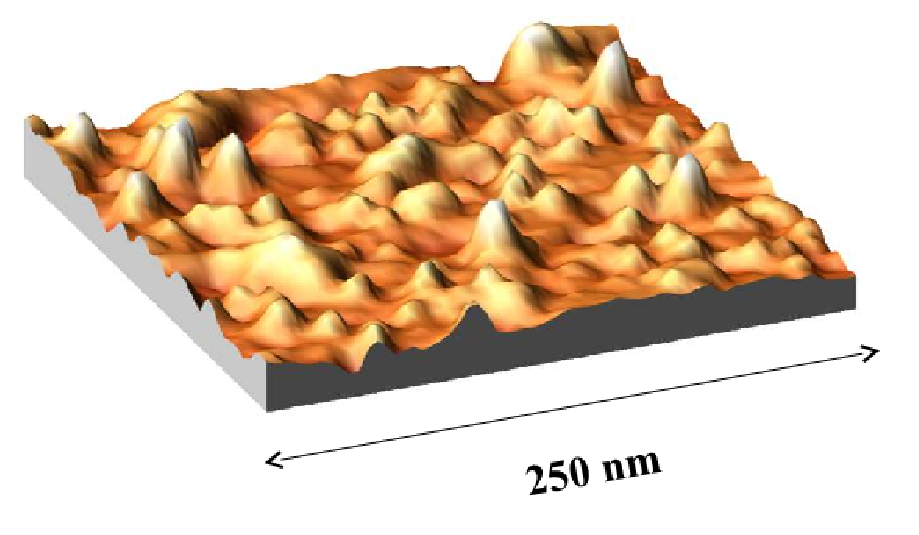
\includegraphics[width=8cm]{01-QD/Pictures/AFMQD.eps}
	\end{center}}
	\end{figure}

	The effects of confinement on the carrier are easier to describe in the envelop function formalism. To define these envelop functions, we develop the carriers wave-functions on all the Bloch states:
	\begin{align}
		\Psi (\mathbf{r}) = \sum_{n,\mathbf{k}} c_{n,\mathbf{k}} \psi_{n,\mathbf{k}} = \sum_{n,\mathbf{k}} c_{n,\mathbf{k}} u _{n,\mathbf{k}} (\mathbf{r}) \exp (i\mathbf{k}.\mathbf{r})
	\end{align}
Since we are in a confined environment, we can consider only the states around $\mathbf{k} = 0$. Since we consider the band extrema, we neglect for this part the inter-band wave function mixing and use the effective-mass approximation. We can then limit the expansion of Bloch state to an expansion on the $u _{n,0} (\mathbf{r}) \exp (i\mathbf{k}.\mathbf{r})$, with $n = \Gamma_6$ for the conduction band and $n = \Gamma_8$ for the valence. We can then write:
	\begin{align}
		\Psi_c (\mathbf{r}) & \simeq \sum_{\mathbf{k}} c_{\mathbf{k}} u _{\Gamma_6,0} (\mathbf{r}) \exp (i\mathbf{k}.\mathbf{r}) = F_e (\mathbf{r}) u _{\Gamma_6,0} \label{eEnvFunc} \\		
		\Psi_v (\mathbf{r}) & \simeq \sum_{J_z = \{\pm \frac{3}{2}, \pm \frac{1}{2}\}, k} c_{J_z,\mathbf{k}} u _{\Gamma_8,J_z} (\mathbf{r}) \exp (i\mathbf{k}.\mathbf{r})  = \sum_{J_z = \{\pm \frac{3}{2}, \pm \frac{1}{2}\}} F_{J_z} (\mathbf{r}) u _{\Gamma_8,J_z} \label{hEnvFunc}
	\end{align}
with $F_e (\mathbf{r}) = \sum_{\mathbf{k}} c_{\mathbf{k}} \exp (i\mathbf{k}.\mathbf{r})$ the electron envelop function and $F_{J_z} (\mathbf{r}) = c_{J_z,\mathbf{k}} \exp (i\mathbf{k}.\mathbf{r})$, $J_z = \{\pm \frac{3}{2}, \pm \frac{1}{2}\}$ the hole envelop functions.

	The effective mass approximation allows us to replace the periodic crystal potential and the free-electron kinetic energy by the effective Hamiltonian representing the band extrema, using $m_e$ for the conduction band 
and ${\cal H}_L + {\cal H}_{BP}$ for the top of the valence band. Considering the effective mass is the same in CdTe and ZnTe, we can now work with the simple picture of an effective mass carrier with the envelop function defined in Eqs.~\ref{eEnvFunc} and \ref{hEnvFunc}, trapped in a potential $V_e (\mathbf{r})$ for the conduction band or $V_h (\mathbf{r})$ for the valence band, created by the band offset between the two semiconductors. We write the Schrödinger equations for these particles:
	\begin{align}
		\left(\frac{\hbar^2}{2m_e}\Delta \right)F_e (\mathbf{r}) + V_e (\mathbf{r}) F_e (\mathbf{r}) &= E_eF_e (\mathbf{r}) \label{eSchroding} \\
		(\tilde{{\cal H}}_L + \tilde{{\cal H}}_{BP} + V_h (\mathbf{r})) 
			\begin{pmatrix}
				F_{+ \frac{3}{2}} (\mathbf{r}) \\
				F_{+ \frac{1}{2}} (\mathbf{r}) \\
				F_{- \frac{1}{2}} (\mathbf{r}) \\
				F_{- \frac{3}{2}} (\mathbf{r})
			\end{pmatrix}
			&= E_h
			\begin{pmatrix}
				F_{+ \frac{3}{2}} (\mathbf{r}) \\
				F_{+ \frac{1}{2}} (\mathbf{r}) \\
				F_{- \frac{1}{2}} (\mathbf{r}) \\
				F_{- \frac{3}{2}} (\mathbf{r})
			\end{pmatrix}
			\label{hSchroding}
	\end{align}
with $\tilde{{\cal H}}_L$ and $\tilde{{\cal H}}_{BP}$ the hole hamiltonians, opposite to the electron hamiltonians defined in Eq.~\ref{LuttHamil} and \ref{BPHamil}. In $\tilde{{\cal H}}_L$, the $k$-terms transform into a gradient of the envelop function with the form $i\nabla$. For simplicity, the $\tilde{}$ will be dropped in the next equations. The derivation of the effective mass approximation can be found in reference \cite{LuttElecMotion}.

	As pointed out in the end of Sec.~\ref{BPSec}, the gap between lh and hh is wide enough to neglect lh contribution in first approximation. This is called the heavy hole approximation, uncoupling the four differential equations defined in Eq.~\ref{hSchroding}. Only the ground states $|\pm \frac{3}{2}\rangle$ are considered, with the effective mass given by the diagonal term of ${\cal H}_{L}$, noted $m_{h, \parallel}$ in the plane and $m_{h, z}$ along the growth axis. The spin operator $J_x$, $J_y$ and $J_z$ can then be redefined in the heavy-hole space as $j_x$, $j_y$, $j_z$, written with the Pauli matrix looking like $\sigma_x$, $\sigma_y$ and $\sigma_z$.
	
	Even with those two approximations, this problem is still unsolvable analytically. However, it is possible for some chosen potentials. Let's consider a lens like quantum dot, with a radius in the $xy$ plane, noted $\rho$, much larger than its height $L_z$. We can therefore define two different harmonic oscillators: a 2D oscillator $V_{c,v} (\rho)$ in the plane, and a 1D oscillator $V_{c,v} (z)$ along the growth axis:
	\begin{align}
		V_{c,v} (\rho) = 4 \Delta E_{c,v} \frac{\rho ^2}{L_z^2} \\
		V_{c,v} (z) = 4 \Delta E_{c,v} \frac{z^2}{L_z^2}
	\end{align}
with $\Delta E_{c,v}$ the difference of conduction (resp. valence) band energy between the two semiconductors. The potential of the whole quantum dot will the be $V_{c,v} (\mathbf{r}) = V_{c,v} (\rho) + V_{c,v} (z)$. Separating the potential in those two parts means we are searching for solution of the form $F(z, \rho, \theta) = \chi (z) \phi_{n,m} (\rho, \theta)$, with $\theta$ the angle between the position vector and the $x$ axis.

	We write the characteristic spatial width $\sigma$ and characteristic frequency $\omega$ of the 2D harmonic oscillator felt by the hole:
	\begin{align}
		\Sigma_{\rho}^h &= \sqrt{\frac{\hbar}{m_{h, \parallel} \omega_{\rho}^{h}}} \\
		\omega_{\rho}^{h} &= \sqrt{\frac{8\Delta E_{v}}{m_{h, \parallel} L_{\rho}^2}}
	\end{align}
We can write the same equality along $z$ replacing $\rho$ by $z$ and $m_{h, \parallel}$ by $m_{h,z}$. The same can be done for electron, replacing the  $m_{h, \parallel}$ or $m_{h,z}$ by $m_e$ and $E_v$ by $E_c$.

	We can find in textbook such as ref.~\cite{MecQBasvant} the solution of a harmonic oscillator from which we can deduce the solution for the ground state (GS) and the first two degenerated excited states. The first excited state is found to have an angular momentum $l_z = \pm 1$, and is then noted $Exc, \pm 1$. The envelop functions and energy are then found to be:
	\begin{align}
			& F_{c,v}^{GS} (z, \rho, \theta) = \frac{1}{(\sqrt{\pi}\Sigma_z)^{\frac{1}{2}}} \exp \left(- \frac{z^2}{2 \Sigma_z^2}\right) \frac{1}{(\sqrt{\pi}\Sigma_{\rho})^{\frac{1}{2}}} \exp \left(- \frac{\rho^2}{2 \Sigma_{\rho}^2}\right) \label{GSWF} \\
			& E_{e,h}^{GS} = \hbar \frac{\omega_z^{e,h} + \omega_{\rho}^{e,h}}{2} \\
		\nonumber \\
			& F_{c,v}^{Exc, \pm 1} (z, \rho, \theta) = \frac{1}{(\sqrt{\pi}\Sigma_z)^{\frac{1}{2}}} \exp \left(- \frac{z^2}{2 \Sigma_z^2}\right) \frac{1}{(\sqrt{\pi}\Sigma_{\rho})^{\frac{1}{2}}} \exp \left(- \frac{\rho^2}{2 \Sigma_{\rho}^2}\right) \frac{\rho}{\sigma_{\rho}} \exp (\pm i\theta) \label{ExcWF} \\
			& E_{e,h}^{Exc, \pm 1} = \hbar \frac{\omega_z^{e,h} + 3 \omega_{\rho}^{e,h}}{2}
	\end{align}
We see that these energy levels are quantified in a way looking like an isolated atom, as pointed earlier. In reference to the atomic notation, the ground state, lower energy level, is noted $S$ and the two first degenerated level are noted $P$, even though atomic p-states usually are 3 fold degenerated.

	One remarkable feature of the envelop functions is that both GS and the two first excited states present the same envelop along the $z$ axis. The cause is directly the symmetry of the QD: since $L_z \ll L_{\rho}$, $\omega_z^{e,h} \gg \omega_{\rho}^{e,h}$, and since $E_{osc.\ harmo.} = (n+\frac{1}{2})\hbar \omega$, the next possible envelop function along the $z$ axis is at higher energy than the next one in the plane. This geometry is also responsible for the 2 fold degeneracy of the $P$-states.
	
	Both the GS and the excited states are once again degenerated due to the spin of the electron and the hole. The electron is in the conduction band with the $\Gamma_6$ symmetry: it can then take the value $\sigma_z = \pm \frac{1}{2}$ (noted $|\uparrow\rangle$ for $+\frac{1}{2}$ and $|\downarrow\rangle$ for $-\frac{1}{2}$). Since we are in the hh approximation, considering the lh are far enough from the band edge to be negligible, the hole spin can only take the values $J_z = \pm \frac{3}{2}$ (noted $|\Uparrow\rangle$ for $+\frac{3}{2}$ and $|\Downarrow\rangle$ for $-\frac{3}{2}$). As pointed ahead, the hole is defined with the opposed characteristic of the missing electron. For instance, a hole $|\Downarrow\rangle$ corresponds to the absence of a valence electron $\Psi_v (\mathbf{r}) = u_{\Gamma_8, \frac{3}{2}} (\mathbf{r}) F_{\frac{3}{2}} (\mathbf{r})$.
	
	The confinement alone does not change the recombination rules we discussed in Sec.~\ref{k0Descr}. The addition of envelop functions in the carriers wave function adds another selection term:
	\begin{align}
		|\langle \Psi_v | \mathbf{p} | \Psi_c \rangle |^2 = |\langle F_v | F_c \rangle |^2|\langle u_{\Gamma_8, J_z} | \mathbf{p} | u_{\Gamma_6, \sigma_z} \rangle |^2
	\end{align}
The first term is the overlap of the envelop function, making sure the hole and the electron are of the right state: a transition between a $P$ state of the valence band and a $S$ state in the conduction band is then forbidden. The second term is the same as the one studied earlier, and from which we deduced the selection rules.

	
	Approximating the QD potential as harmonic usually overestimate the confinement, and thus the single-particle energy. But the wave-functions found in this chapter can still be used as trial wave-functions for variational calculations in other potential, in order to estimate the correct energy level.
	

		\subsection{Electron-hole exchange in quantum dots\label{ehExch}}
		













	%Bir et Pikus: l'interaction d'échange de coulomb de l'électron CB and les électrons VB peut être séparés en deux terme : un short range et un long range.
	
	Electrons are fermions, and thus are subjected to the Pauli exclusion principle. Being charged particles, they also interact with each other via the Coulomb interaction. Both of those have to be considered to write the interaction between the carriers in the semiconductor. It was shown by Wardzyński et al.~\cite{ExchSplitInteratomic} that the interaction between a conduction electron and all the electrons of the valence band can be written as an interaction between the considered electron and the corresponding hole. It can separated into two term: the direct Coulomb interaction and the exchange Coulomb interaction.
	
	
	In exciton, the direct Coulomb term is attractive, as classically expected from an electric interaction between two opposite charges. However, more complex systems can exist in a semiconductor: charged excitons X$^+$ (hole-hole-electron complex) and X$^-$ (hole-electron-electron complex), or biexciton X$^2$ (two excitons of opposite total angular momentum). Higher order multi-excition or charged biexciton might also exists but they are not discussed in this thesis. For such complex, the direct Coulomb interaction might become attractive for two charges of same sign.

	Taking into account the symmetry of the crystal, Bir and Pikus demonstrated~\cite{BPExchInt} that the exchange hamiltonian between an electron of the conduction band and hole in the valence band can be decomposed in two different components:\newline
	For an electron and a hole in the same Brillouin zone, the short-range exchange interaction is to be considered. It can be written:
	\begin{align}
		{\cal H}_{eh}^{sr} = I_{eh}^{sr} \bm{\upsigma}.\mathbf{j} + \sum_{i = x,y,z} b_i^{exch} \sigma_i j_i^3
	\end{align}
The first term lift the degeneracy between exciton of total angular moment $X=2$ and $X=1$. The second one take into account the reduction of symmetry in a cubic lattice and gives the dark states a fine structure. This have never been observed experimentally in bulk semiconductor, but it is expected to be much smaller than the lift induced by $I_{eh}^{sr}$.\newline
	For carriers in different Brillouin-zone, the long-range exchange interaction have to be considered. In bulk semiconductors, the long range term doesn't affect the bright exciton at $k = 0$. Since the radiative recombination we study occurs at $k=0$, the long range interaction does not affect it.
	
	In a quantum dot, the confinement of the carrier leads to a better overlap of the wave function and thus greater short range exchange energies. Moreover, in an anisotropic potential, such as the one of Stransky-Krastanov dots (see Chap.~II.1), the long-range interaction mixes the bright exciton, splitting them in two levels. 
	%The splitting between the dark and bright excitons is thus also affected.
Taking into account all these effect, we can the write the total hamiltonian in the heavy hole exciton subspace ($X_z = |+2\rangle$, $|+1\rangle$, $|-1\rangle$, $|-2\rangle$):
	\begin{align}
	\label{Heh}
		{\cal H}_{eh} &=
		\begin{pmatrix}
			\delta_0 & 0 & 0 & \delta_2 \\
			0 & - \delta_0 & \frac{1}{2} \delta_1 \exp(-2i \phi_1) & 0 \\
			0 & \frac{1}{2} \delta_1 \exp(-2i \phi_1) & -\delta_0 & 0 \\
			\delta_2 & 0 & 0 & \delta_0
		\end{pmatrix}
	\end{align}
with $\delta_0 = \frac{3}{2}I_{eh}$ representing the splitting between dark and bright exciton, $\delta_1$ the splitting between the bright exciton states and $\delta_2$ the dark exciton states fine structure. $\delta_0$ value is controlled both by long-range and short-range interaction, and is typically of about 1 meV in CdTe/ZnTe. $\delta_1$ only appear in anisotropic quantum dot and is induced by the long-range interaction, varying between a few tens and a few hundreds of $\mu$eV. Finally, $\delta_2$ primarily arise from the short-range interaction.

	
	Calculating the eigenstate of the hamiltonian \ref{Heh}, we find that the optically active states are linearly polarized along $\varphi_1$ and $\varphi_1 + 90^{\circ}$ as followed:
	\begin{align}
		|\pi_{\varphi_1}\rangle = \frac{1}{\sqrt{2}}\left(\exp(-i\varphi_1)|+1\rangle + \exp(i\varphi_1)|-1\rangle\right) \\
		|\pi_{\varphi_1 + 90^{\circ}}\rangle = \frac{1}{\sqrt{2}}\left(\exp(-i\varphi_1)|+1\rangle - \exp(i\varphi_1)|-1\rangle\right)
	\end{align}
In order to get a polarization of the emission along the 110 axis, we choose $\varphi_1 = \dfrac{\pi}{4}$.

	This model works well for quantum dots with an elongated lens shape ($C_{2v}$ symmetry).  However, more realistic self-assembled quantum dots have symmetries which can deviate quite substantially from the idealized shapes of circular or ellipsoidal lenses. For a $C_{s}$ symmetry (truncated ellipsoidal lens), additional terms coupling the dark and the bright excitons have to be included in the electron-hole exchange Hamiltonian. Following Ref. \cite{ZielinskiDarExc}, the general form of the electron-hole exchange Hamiltonian in the heavy-hole exciton basis for a low symmetry quantum dot (C$_s$) is
	\begin{align}
		\label{HehCs}
		\mathcal{H}_{eh} =\frac{1}{2} \left(
			\begin{array}{cccc}
			\delta_0                               &e^{-i\pi/4}\delta_{11}              &e^{i\pi/4}\delta_{12}        &\delta_2\\
			e^{i\pi/4}\delta_{11}                      &-\delta_0                       &e^{-i\pi/2}\delta_{1}       &-e^{i\pi/4}\delta_{12}\\
			e^{-i\pi/4}\delta_{12}                  &e^{i\pi/2}\delta_{1}           &-\delta_0                     &-e^{-i\pi/4}\delta_{11}\\
			\delta_2                 &-e^{-i\pi/4}\delta_{12}          &-e^{i\pi/4}\delta_{11}                     &\delta_0\\
			\end{array}
		\right)
\end{align}
		
		
		\subsection{Valence band mixing\label{VBM}}	
	
	The long range exchange interaction split the neutral exciton bright states in two linearly polarized lines, with a $90^{\circ}$ angle between them. However, this simple picture doesn't fit well with the data, such as presented in Fig.~\ref{XAlLinPol}. For once, it is clear for the neutral species ($X$, $X^2$) that the angle between the polarization of the two lines is different from $90^{\circ}$. Moreover, the charged species ($X^+$, $X^-$) are found to present linear polarization dependency, when the presence of the second hole ($X^+$) or electron ($X^-$) with an opposite spin should compensate the exciton exchange interaction, and thus these system should not present any dependency in linear polarization.
	
	\begin{figure}[h!]
	\begin{center}
		\includegraphics[width=13cm]{01-QD/Pictures/LinPol.png}
	\end{center}
	\caption{PL intensities of the lines of the bi-exciton, the charged excitons and the neurtral exciton of CdTe/ZnTe quantum dot as the function of the angle of the linearly polarized detection. To simplify the reading, the intensities were also plotted on polar graph (bottom). Picture taken from Yoan L\'eger PhD thesis~\cite{YoanTh}.}
	\label{XAlLinPol}
	\end{figure}
	
	In order to fully understand it dependency, we have to stop neglecting the light hole contribution. Looking at the general form of the Luttinger hamiltonian \ref{HLMat}, we see that it mixes heavy hole and light hole through its non-diagonal term $b_{Lutt}$ and $c_{Lutt}$. The Bir-Pikus hamiltonian \ref{BPHamil} presents the same symmetry and the same form as the Luttinger hamiltonian and thus also induces a coupling between the lh states and the hh states. In general, we can write the hamiltonian describing the influence of shape and strain on the valence structure in the ($|\dfrac{3}{2}, +\dfrac{3}{2}\rangle$, $|\dfrac{3}{2}, +\dfrac{1}{2}\rangle$, $|\dfrac{3}{2}, -\dfrac{1}{2}\rangle$, $|\dfrac{3}{2}, -\dfrac{3}{2}\rangle$) basis as:	
	\begin{align}
	\label{HVBM}
		{\cal H}_{VBM} =
		\begin{pmatrix}
			p+q & s & r & 0 \\
			s^* & p-q & 0 & r \\
			r^* & 0 & p-q & -s \\
			0 & r^* & -s^* & p+q
		\end{pmatrix}				
	\end{align}
The induced hh/lh mixing is called Valence Band Mixing (VBM).

	Supposing a VBM only caused by strain anisotropy, through the Bir-Pikus hamiltonian, we can write these parameters as function of the Bir-Pikus parameters and the crystal deformation $\varepsilon_{ij}$ ($i,j = x$, $y$, $z$) with $x$ the (100) axis of the crystal lattice and $z$ as defined above. The VBM parameters then writes as follow~\cite{kpMethod}:
	\begin{align}
		p 	&= a_v Tr(\varepsilon) \\
		q	&= b \left(\varepsilon_{zz} - \frac{\varepsilon_{xx} + \varepsilon_{yy}}{2}\right) \\
		r	&= b \frac{\sqrt{3}}{2} (\varepsilon_{xx} - \varepsilon_{yy}) - id \varepsilon_{xy} \\
		s	&= d(\varepsilon_{xz} - i\varepsilon_{yz})
	\end{align}
The splitting between the hh states and the lh states can now be calculated in function of the Bir-Pikus parameters:
	\begin{align}
		\begin{array}{rl}
			\Delta_{lh} &= E_{\pm\frac{3}{2}} - E_{\pm\frac{1}{2}} = (p+q) - (p-q) \\
						&= 2b \left(\varepsilon_{zz} - \dfrac{\varepsilon_{xx} + \varepsilon_{yy}}{2}\right)
		\end{array}
	\end{align}
	
	If we now suppose a system with pure in-plane strain anisotropy ($Q=0$), for an origin of the energy at the top of the valence band, i.e. the hh band, we can rewrite the VBM hamiltonian in the same basis as above as:
	\begin{align}
		{\cal H}_{VBM}^{in\ plane} =
		\begin{pmatrix}
			0 & 0 & \rho_s\exp(-2i\theta_s) & 0 \\
			0 & \Delta_{lh} & 0 & \rho_s\exp(-2i\theta_s) \\
			\rho_s\exp(2i\theta_s) & 0 & \Delta_{lh} & 0 \\
			0 & \rho_s\exp(2i\theta_s) & 0 & 0
		\end{pmatrix}
	\end{align}
with $\rho_s$ the strain coupling amplitude and $\theta_s$ the angle between axis of the strain induced anisotropy in the QD plane and the $x$ axis. One can notice that in the case of pure in-plane anisotropy, $|+\dfrac{3}{2}\rangle$ only mixes with $|-\dfrac{1}{2}\rangle$ and $|-\dfrac{3}{2}\rangle$ with $|+\dfrac{1}{2}\rangle$. An anisotropy along the $z$ axis, growth axis of the dots, is needed to mix $|\pm \dfrac{3}{2}\rangle$ with $|\mp \dfrac{1}{2}\rangle$. With this notation, in the limit of weak VBM, we can now rewrite the ground state of the holes as pseudo-spin in order to take the hh/lh mixing into account:
	\begin{align}
		|\tilde{\Uparrow}\rangle \propto |+\frac{3}{2}\rangle - \frac{\rho_s}{\Delta_{lh}}\exp(2i\theta_s)|-\frac{1}{2}\rangle \\
		|\tilde{\Downarrow}\rangle \propto |-\frac{3}{2}\rangle - \frac{\rho_s}{\Delta_{lh}}\exp(-2i\theta_s)|+\frac{1}{2}\rangle
	\end{align}
And we have to define new angular momentum operator for these pseudo-spin:
	\begin{align}
		\tilde{J}_+ &= \frac{\rho_s}{\Delta_{lh}}
			\begin{pmatrix}
				0 & -2\sqrt{3}\exp(-2i\theta_s) \\
				0 & 0
			\end{pmatrix} \label{JtildeUP} \\
		\tilde{J}_- &= \frac{\rho_s}{\Delta_{lh}}
			\begin{pmatrix}
				0 & 0 \\
				-2\sqrt{3}\exp(2i\theta_s) & 0
			\end{pmatrix} \label{JtildeDOWN} \\
		\tilde{J}_z &=
			\begin{pmatrix}
				\dfrac{3}{2} & 0 \\
				0 & -\dfrac{3}{2}
			\end{pmatrix}
	\end{align}
$\tilde{J}_{\pm}$ are the ladder operators, flipping the hole spin, whereas $\tilde{J}_z$ return the spin value. This last operator confirm these states are mainly hh. This pseudo spin description is enough in most of the case to understand the effect of the VBM, and we will use it to study how it modify the emission of the quantum dot.

	%\end{align}

	In order to do so, we begin to consider the emission of an charged state. Since, as explained earlier, the exchange interaction is null is such systems, it will allows us to focus only on the VBM effect. We can ignore the envelop function, testing mainly the overlap of the carriers wave function and thus not affecting the polarization of the emission. We write the polarization of the detection $\mathbf{e} = \cos (\alpha) \mathbf{e_x} + \sin (\alpha) \mathbf{e_y}$. We then can find the oscillator strength of the transition:
	\begin{align}		
		\begin{array}{rl}
		\label{VBMPolar}
			\Omega (\alpha) &\propto |\langle \uparrow | \cos(\alpha)p_X + \sin(\alpha)o_Y | \uparrow \downarrow \tilde{\Uparrow} \rangle |^2 \\
							&= 1 + \dfrac{1}{3} \dfrac{\rho_s}{\Delta_{lh}}^2 + \dfrac{2}{\sqrt{3}} \dfrac{\rho_s}{\Delta_{lh}} \cos(2(\theta_s - \alpha))
		\end{array}
	\end{align}
with $\mathbf{p} = -i\hbar\bm{\nabla}$. Contrary to what is expected in the hh approximation, we see that the charged exciton can have a strong linear component, depending on the strength of the lh/hh mixing.

	In the QD presented in Fig.~\ref{XAlLinPol}, the linear polarization rate $\rho_l = \dfrac{2A}{1 + A^2} \approx 40\%$, with $A = \frac{\rho_s}{\sqrt{3}\Delta_{lh}}$ corresponding to a very strong lh-hh mixing, with $\frac{\rho_s}{\Delta_{lh}} \approx 0.75$. Experimentally, no correlation were found between the polarization axis of different QDs, even if they are close to each other, neither with the crystallographic axis. Such a behaviour can be explained considering the anisotropic relaxation of strains occurring during the growth of our QDs~\cite{VBMArticle}. This behaviour was also observed in III-V compounds at low QD density (near the 2D-3D transition), also attributed to the effect of strains~\cite{IIIVFastExcSpinRelax}. For the III-V system, this hypothesis is supported by AFM studies showing that, in such growth conditions, the dots are preferentially nucleating near structural defects~\cite{IIIVAFM}. In the case of II-VI materials, a strained induced hh/lh mixing us not surprising as the dislocation formation energy is lower~\cite{TinjodMBE}.

	For the charged states $X^+$ and $X^-$, only the VBM lead to this linear polarization, leading to the simple picture discussed in this section. However, in $X$ and $X^2$, the VBM and the long range exchange interaction are in competition for the polarization of the emission. The strains tend to polarized it along $\theta_s$ and $\theta_s + 90^{\circ}$, when the long range exchange interaction favour linear emission along $\varphi_1$ and $\varphi_1 + 90^{\circ}$. This explains that the angle between the two linearly polarized exciton lines is not equal to $90^{\circ}$. Moreover, the valence band mixing results in a fine structure splitting through the short range exchange interaction that can either enhance or decrease the fine structure splitting due to the long range exchange interaction. In order to illustrate our point, we consider only the isotropic part of the short range exchange interaction between the electron and the light or heavy hole:
	\begin{align}
		{\cal H}_{eh}^{sr,iso} = I_{eh} \bm{\upsigma}.\mathbf{J}
	\end{align}
where $\frac{3}{2}I_{eh}$ corresponds to the energy splitting between bright and dark excitons due to the short range exchange interaction. The coupling between the bright states $|\downarrow \tilde{\Uparrow}\rangle$ and $|\uparrow \tilde{\Downarrow}\rangle$ through ${\cal H}_{eh}^{sr,iso}$ can be calculated using the pseudo-spin ladder operator defined in \ref{JtildeUP} and \ref{JtildeDOWN}:
	\begin{align}
		\langle \downarrow \tilde{\Uparrow} | {\cal H}_{eh}^{sr,iso} | \uparrow \tilde{\Downarrow}\rangle = \frac{1}{2\sqrt{3}} I_{eh} \frac{\rho_s}{\Delta_{lh}} \exp(-2i\theta_s)
	\end{align}
	
	Hence, the valence band mixing through the short range exchange interaction splits the bright states into two linearly polarized states along axis defined by the strain angle $\theta_s$. The competition between this effect and the long range exchange interaction results in an angle between the two linearly polarized states different from $90^{\circ}$, as observed in the emission of CdTe/ZnTe QDs~\cite{DELum} and in InAs/GaAs ones~\cite{PolarIIIV}. Dark states are also coupled to each other in second order, giving them a weak oscillator strenght, with a dipole along $z$. A more in depth investigation of these effects was done in Yoan L\'eger PhD thesis~\cite{YoanTh}.

	
	\section{Exchange interaction between carrier and magnetic atom\label{Exch}}
	
		\subsection{Exchange interaction in Diluted Magnetic Semiconductors\label{ExchDMS}}
		
		We looked until now at the structure of a so-called perfect semiconductor, without defect or impurity. However, we are interested in thesis to introduce a low density of either Manganese or Chromium atoms in the crystal, namely, impurities. A semiconductor doped in this fashion is called Diluted Magnetic Semiconductor (DMS). This magnetic atom will interact with the semiconductor electrons via its localized electrons on its exterior shell. For Mn and Cr in CdTe, this orbital is the $d$ orbital, so it will be the one considered in the following document. From the interactions between these electrons and the one in the conduction band of the semiconductor, new properties will arise. We will try in this chapter to write this interaction as a "Heisenberg" interaction:
		\begin{align}
			{\cal H}_{Heisenberg} = I \bm{\upsigma}.\mathbf{S}
		\end{align}
with $I$ the interaction constant, $\bm{\upsigma}$ the electron spin and $\mathbf{S}$ the spin of the magnetic atom.
	
	This formally simple interaction represents the Pauli exclusion principle through the interaction between two spins. Almost all the interactions in this chapter will be of this form, although presenting different physical processes, with only the interaction constant $I$ varying from one another.
	
	Both Cr and Mn are close in size to the Cd atoms they replace, so their insertion only induces a small perturbation in the crystal structure, meaning the semiconductor wave function will not be significantly altered by them. We can then as usual note the conduction electron wave function as $|\psi_{\mathbf{k}}\rangle|\sigma;\sigma_z\rangle \equiv |\psi_{\mathbf{k}};\sigma_z\rangle$, $|\psi_{\mathbf{k}}\rangle$ being the Bloch function of the semiconductor. On the other side, considering a magnetic atom at $\mathbf{r} = \mathbf{R_d}$, we write the spatial component of the wave function $\Phi_d (\mathbf{r} - \mathbf{R_d})$. Its total electronic spin, sum of the electron spins on its $d$ orbital, is noted $|S; S_z\rangle$. The whole wave function of the magnetic atom is then $|\Phi_d;S_Z\rangle$.
	
	Using Born-Oppenheimer approximation, we can write the hamiltonian for these electrons:
	\begin{align}
	\label{BOHamil}
		{\cal H}_{BO} = \sum_i \left(\frac{p_i^2}{2m_c} + V_c (\mathbf{r}_i) \right) + \frac{1}{2} \sum_{i,j} \frac{e^2}{4\pi \varepsilon_0 |\mathbf{r_i} - \mathbf{r_j}|}
	\end{align}
The first term is a single particle hamiltonian, taking into account the kinetic energy of the electron and the crystal potential $V_c (\mathbf{r}_i)$ felt by the electron at the position $\mathbf{r}_i$. This potential includes the impurities' potential, meaning it will be different at the impurities positions rather than elsewhere in the semiconductor. The final term represents the Coulomb interaction between the electrons.

	We can rewrite this hamiltonian using second quantification. We define the destruction (resp. creation) operator of a particle in the conduction band at the wave vector $\mathbf{k}$ and the spin $\sigma$ as $a_{\mathbf{k}, \sigma}$ (resp. $a_{\mathbf{k}, \sigma}^{\dagger}$). In the same fashion, we define the destruction (resp. creation) operator of the electronic level of an impurity as $a_{d, S}$ (resp. $a_{d, S}^{\dagger}$). Supposing the number of electrons on the $d$ orbital of the considered magnetic atom does not change, the hamiltonian \ref{BOHamil} then become:
	\begin{align}
			{\cal H}_{SQ} &= \sum_{\mathbf{k}, \sigma} E_{\mathbf{k}} a_{\mathbf{k}, \sigma}^{\dagger} a_{\mathbf{k}, \sigma} + \sum_{S} E_d a_{d, S}^{\dagger} a_{d, S} + \sum_{\mathbf{k}, \mathbf{k}'} U_{\mathbf{k}, \mathbf{k}'} a_{\mathbf{k}, \sigma}^{\dagger} a_{\mathbf{k}', \sigma} \nonumber \\
								&\qquad\qquad\quad+ \sum_{\mathbf{k}, \sigma, S} M_{\mathbf{k}} (a_{\mathbf{k}, \sigma}^{\dagger} a_{d, S} + a_{d, S}^{\dagger} a_{\mathbf{k}, \sigma}) + \frac{1}{2} \sum_{i,j,k,l} V_{i,j,m,n} a_i^{\dagger} a_j^{\dagger} a_n a_m \label{HamilSQ} \\
						&= {\cal H}_0 + {\cal H}_d + V_d + {\cal H}_{hyb} + {\cal H}_{Coulomb} \nonumber
	\end{align}
The constant electron number supposition is good enough for the picture we want to draw since most of the spin-driven interactions do not induce a change of this number.

	${\cal H}_0$ represents the energy of the unperturbed wave function of the semiconductor, with $E_k$ the energy of an electron with the wave vector $\mathbf{k}$.
	
	${\cal H}_d$ is the same as ${\cal H}_0$ but for an electron of the $d$ orbital of the considered magnetic impurity, with $E_d$ the energy of an electron on this orbital.
	
	$V_d$ represents the impurities potential, allowing the semiconductor electrons to scatter on it. However, Mn and Cr does not modify strongly the crystal potential. We can then consider that the states of the semiconductor $|\psi_k\rangle$ are also solution of the full crystal potential, including impurity, and neglect this term.
	
	${\cal H}_{hyb}$, also called the Anderson hamiltonian, mixes the semiconductor states with the states of the impurities. It represents an exchange interaction between an electron of the semiconductor and one of the $d$ orbital of an impurity. We can write the exchange constant as:
	\begin{align}
	\label{Vkd}
		V_{kd} = \int \mathrm{d}\mathbf{r} \psi_k^* (\mathbf{r}) {\cal H}_1 \Phi_d (\mathbf{r} - \mathbf{R_d})
	\end{align}
with ${\cal H}_1$ the one particle hamiltonian. This term depends on the Bloch state of both the semiconductor and the impurity, meaning it can be reduced to zero by the symmetry of such functions in some specific cases.

	Let's now focus on last term, ${\cal H}_{Coulomb}$, representing the two particles exchange. $i$, $j$, $m$ and $n$ each represents a full wave function, both spatial and spin part, and can be either an electron of the semiconductor or of one of the impurities. We can then separate this hamiltonian in three different terms depending on the value of $i$, $j$, $m$ and $n$ and illustrated in Fig.~\ref{HybridEner}.
	

	\begin{figure}[h!]
	\fcapside{\caption{Carrier interactions with no change of the number of electrons on the impurity, derived from the hamiltonian ${\cal H}_{Coulomb}$. Picture from Laurent Maingault PhD thesis~\cite{LaurentTh}.}\label{HybridEner}}
	{\begin{center}
		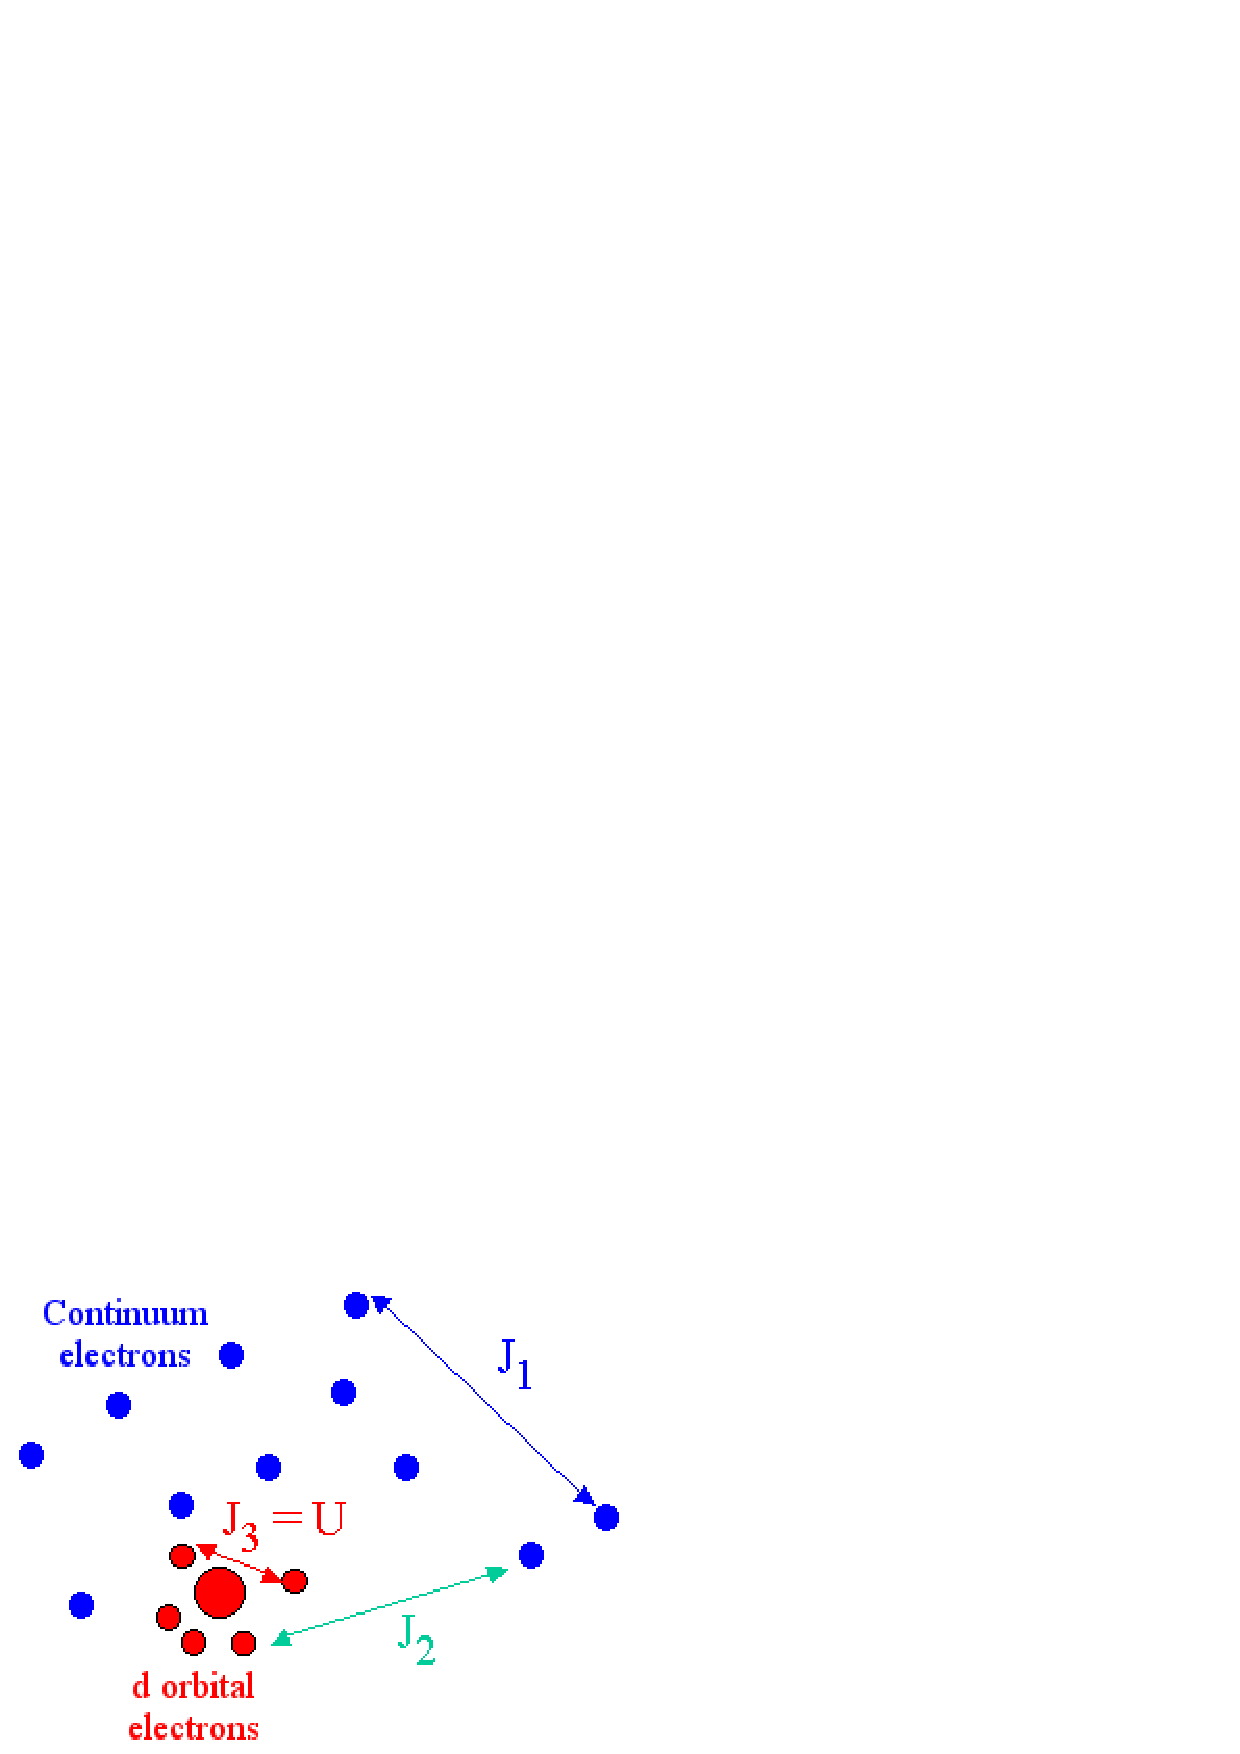
\includegraphics[width=6cm]{01-QD/Pictures/ExchInt.png}
	\end{center}}
	\end{figure}

	We first consider two states belonging to the continuum, appearing as $J_1$ on the diagram. This is the hamiltonian $H_{eh}$ introduced in Sec.~\ref{ehExch}.

	
	The next interaction we consider is the one of two electrons from a localized atom. It represents internal transitions of the atom, representing the Hund rule. It is written:
	\begin{align}
		{\cal H}_U = \sum_{d, S, S'} U a_{d, S}^{\dagger} a_{d, S'}^{\dagger} a_{d, S'} a_{d, S'}
	\end{align}
with $U = \int \mathrm{d}\mathbf{r} \mathrm{d}\mathbf{r'} \dfrac{e^2}{4\pi\varepsilon_0 |\mathbf{r} - \mathbf{r'}|} |\Phi_d (\mathbf{r})|^2 |\Phi_d (\mathbf{r'})|^2$ the Coulomb interaction between two electrons on the same orbital with different spins. Thus, it costs more energy to add an electron on the same orbital than on another. We find back the Hund rule, with electrons first filing all orbitals with parallel spin before adding an electron to an orbital with another one, with opposed spin.
	
	The third considered interaction is the one between an electron from the magnetic atom and an electron from the semiconductor. In the same fashion as with carriers of the bulk, it can be separated in two terms that will be developed in the next paragraphs: a direct Coulomb interaction between the two electrons, and an exchange interaction arising from the fermionic nature of electrons.
	
	The direct Coulomb interaction doesn't depends on electrons spins. It only act on the total energy of the system and is therefore only needed when searching the total energy of an exciton. We write it:
	\begin{align}
		K &= + \sum_{\mathbf{k}, \sigma, \sigma'} K_{\mathbf{k}} a_{\mathbf{k}, \sigma}^{\dagger} a_{d, \sigma'}^{\dagger} a_{d, \sigma'} a_{\mathbf{k}, \sigma} \\
		\text{with} \nonumber \\
		K_k &= \int \mathrm{d} \mathbf{r} \mathrm{d} \mathbf{r}' |\psi_k (\mathbf{r})|^2 \frac{e^2}{4\pi \varepsilon_0 |\mathbf{r}' - \mathbf{r}|} |\Phi_d (\mathbf{r}')|^2 \nonumber
	\end{align}
It is clear that the spin $\sigma$ (resp. $\sigma'$) of the $k$ electron (resp. $d$ electron) is not changed by this interaction. Since it only induce a shift in the total energy, we can redefine the origin of the energy axis to ignore it.

	To go to the second term, the exchange interaction, we write it in second quantification:
		\begin{align}
			J &= + \sum_{k, k', \sigma, \sigma'} I_{kk'}^{ex} a_{k', \sigma}^{\dagger} a_{d, \sigma'}^{\dagger} a_{k, \sigma'} a_{d, \sigma} = + \sum_{k, k', \sigma, \sigma'} J_{kk'} a_{k', \sigma}^{\dagger} a_{k, \sigma'} a_{d, \sigma'}^{\dagger} a_{d, \sigma} \label{sdSQ} \\
			\text{with} \nonumber \\
			I_{kk'}^{ex} &= \int \mathrm{d} \mathbf{r} \mathrm{d} \mathbf{r}' \psi_{k'}^* (\mathbf{r}) \psi_{k}^* (\mathbf{r}') \frac{e^2}{4\pi \varepsilon_0 |\mathbf{r}' - \mathbf{r}|} \Phi_{d}^* (\mathbf{r}) \Phi_{d}^* (\mathbf{r}') \label{sdConst}
		\end{align}
As can be sawn on Eq.~\ref{sdSQ}, this interaction exchange the spin $\sigma$ and $\sigma'$ of both electrons, thus its name. Eq.~\ref{sdConst} shows that the spin interaction comes from a Coulomb interaction between two fermions.

	We define:
		\begin{align}
			\begin{array}{l}
				\sigma_{kk'}^z = a_{k, \sigma}^{\dagger} a_{k', \sigma} - a_{k, -\sigma}^{\dagger} a_{k', -\sigma} \\
				\sigma_{kk'}^+ = a_{k, \sigma}^{\dagger} a_{k', -\sigma} \\
				\sigma_{kk'}^- = a_{k, -\sigma}^{\dagger} a_{k', \sigma}
			\end{array}
		\end{align}
Considering now that this interaction does not change the number of electrons on the $d$ orbital of the considered magnetic atom, we can find the Kondo hamiltonian:
	\begin{align}
		{\cal H}_{sd} = - \sum_{k, k'} I_{kk'}^{ex} \bm{\upsigma}_{k,k'}.\mathbf{S}
	\end{align}
Since $I_{k,k'}^{ex}$ is positive, the negative sign in front of the Kondo hamiltonian shows that the energy minimum is reached when the spins of both electrons are aligned, and is therefore ferromagnetic.
	
	We can now write the hamiltonian \ref{HamilSQ}, detailing these new hamiltonians:
		\begin{align}
			{\cal H}_{SQ} &= {\cal H}_0 + {\cal H}_d + {\cal H}_{hyb} + {\cal H}_{eh} + {\cal H}_{U} + {\cal H}_{sd}
		\end{align}
with the exchange constant in ${\cal H}_{hyb}$, $V_{kd} = \int \mathrm{d}\mathbf{r} \psi_k^* (\mathbf{r}) {\cal H}_1 \Phi_d (\mathbf{r} - \mathbf{R_d})$.

	We now have two hamiltonians to model the exchange interaction between the impurities electrons and the one in the conduction band of the semiconductor: ${\cal H}_{hyb}$ and ${\cal H}_{sd}$. Schrieffer and Wolff rewrote the Anderson hamiltonian in order to give a form closer to the Kondo hamiltonian~\cite{RelationAnderKondo}:
	\begin{align}
	\label{Ikk'}
			{\cal H}_{hyb} &= ( \sum_{k,k'} V_{kd} V_{k'd} \left(\dfrac{1}{E_k - (E_d + U)} + \dfrac{1}{E_{k'} - (E_d + U)}\right. \nonumber \\
			 				& \qquad \qquad \qquad \qquad \qquad \qquad \left. - \dfrac{1}{E_k - E_d} - \dfrac{1}{E_{k'} - E_d}\right)a_{k', \sigma}^{\dagger} a_{k, -\sigma} a_{d, S-2\sigma}^{\dagger} a_{d, S} \nonumber \\
			 				&= -  \sum_{k,k'} I_{kk'}^{hyb} a_{k', \sigma}^{\dagger} a_{k, -\sigma} a_{d, S-2\sigma}^{\dagger} a_{d, S}
	\end{align}
The Fig.~\ref{EnerTransit} illustrates the different energies introduced in \ref{Ikk'}, presenting virtual transitions to the $d$ orbital of the magnetic atom. The two possible energies are $E_d$ for the low energy level, and $E_d + U$ for the high energy one, $U$ being the energy needed to add an electron to the orbital.

	\begin{figure}[h!]
	\begin{center}
		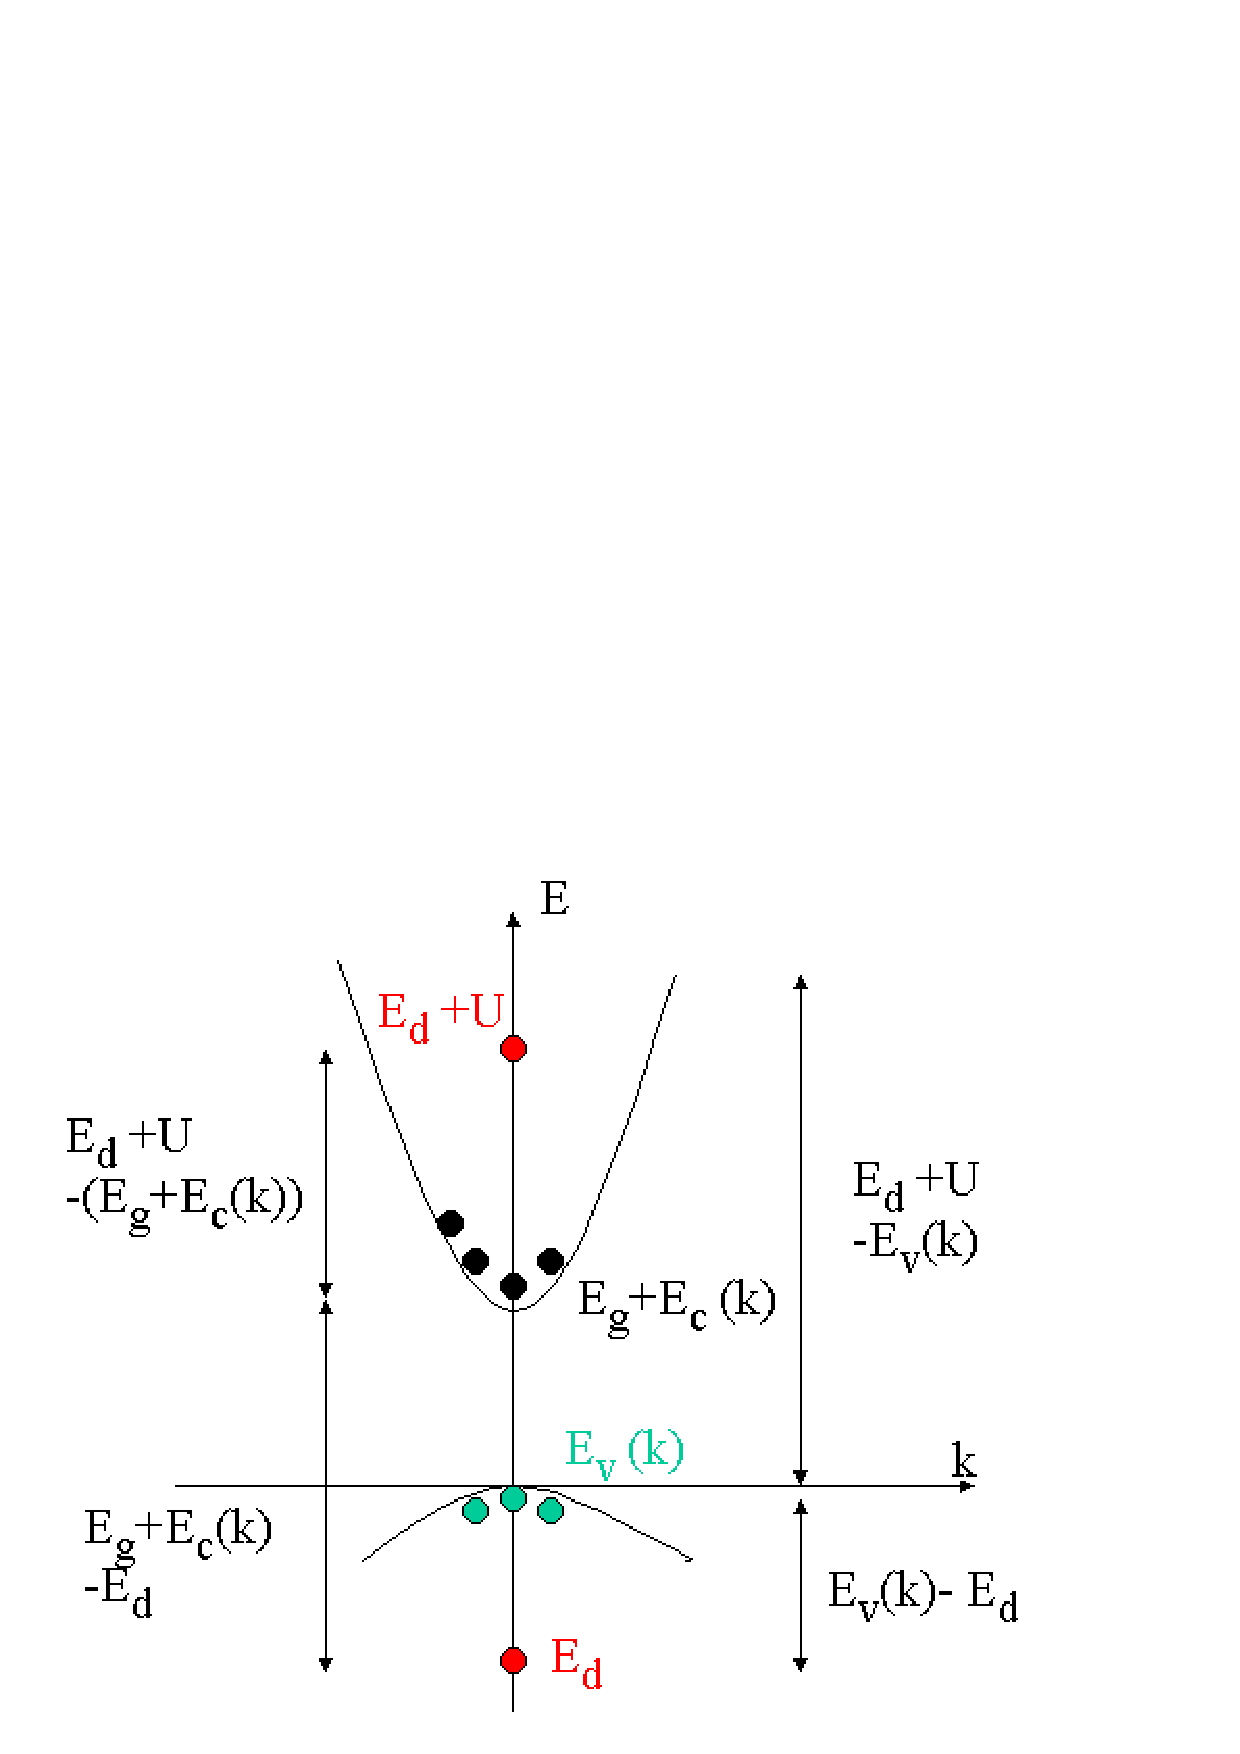
\includegraphics[width=10cm]{01-QD/Pictures/EnergyLevels.png}
	\end{center}
	\caption{Schema of the band structure and virtual transitions between valence band and conduction band. Picture from Laurent Maingault PhD thesis~\cite{LaurentTh}.}
	\label{EnerTransit}
	\end{figure}

	Doing this transformation is an important step, since we are now able to use a Heisenberg type spin hamiltonian instead of a hamiltonian mixing wave functions, in addition to having the same formalism to write both type of exchange interactions, with just a difference in the exchange constants $I_{kk'}^{ex}$ and $I_{kk'}^{hyb}$.

	Supposing the coupling occurs between two electrons with a close $k$ ($k \simeq k'$), we can rewrite $I_{kk'}^{hyb}$ as:
	\begin{align}
		\begin{array}{rl}
			I_{kk'}^{hyb} &= 2|V_{kd}|^2 \dfrac{U}{(E_k - E_d)(E_k - (E_d + U)} \\
						&= -2|V_{kd}|^2 \dfrac{U}{(E_k - E_d)(E_d + U - E_k})
		\end{array}
	\end{align}
Fig.~\ref{EnerTransit} presents the case where the magnetic atom ground state is deep inside the valence band. This is the case for the Mn atom. In this case, one can see that $U$ and $E_k - E_d$ are both positive, while $E_k - (E_d + U)$ is negative. Thus, $I_{kk'}^{hyb}$ is negative, and we see that, while exchange leads to a ferromagnetic coupling, hybridization leads to an anti-ferromagnetic one. There will be a competition in the semiconductor between these two for every type of carrier.

	The Cr case is more complicated: its ground state is at the limit between the gap and the conduction band. Therefore, knowing the sign of $E_k - E_d$ and $E_k - (E_d + U)$ is more difficult. It will be discussed more in details in its dedicated part in Sec.~\ref{CrCdTe}.

	Using the same hypothesis done on Sec.~\ref{BandStruct} of small $k$ value, and the value of $V_{kd}$ presented in Eq.~\ref{Vkd}, we can rewrite the exchange constant:
	\begin{align}
		I_{00, \{c,v\}}^{hyb} &= -2 \left(\frac{U}{(E_{\{c,v\}}(0) - E_d)(E_d + U - E_{\{c,v\}}(0))}\right) \int \mathrm{d}\mathbf{r} \Phi_r^* (\mathbf{r}) {\cal H}_1 \psi_0^{\{c,v\}} \\
		I_{00, \{c,v\}}^{ex} &= \int \mathrm{d}\mathbf{r} \mathrm{d}\mathbf{r}' \psi_0^{*\{c,v\}} (\mathbf{r}) \Psi_d^* \frac{e^2}{4\pi \varepsilon_0 |\mathbf{r}' - \mathbf{r}|\psi_0^{\{c,v\}} (\mathbf{r}) \Psi_d} (\mathbf{r})
	\end{align}
In the valence band, the semiconductor's atoms exterior orbitals have the $p$ symmetry, as discussed in Sec.~\ref{BandStruct}. We then write $I_{pd}$ as the sum of the hybridization and the exchange contributions:
	\begin{align}
		I_{pd} =I_{00, v}^{hyb} +  I_{00, v}^{ex}
	\end{align}
In the conduction band, the orbitals are $s$, and so we will write the interaction $I_{sd}$. However, since $s$ orbitals have a spherical symmetry, there is no hybridization contribution. The expression is then pretty easy:
	\begin{align}
		I_{sd} = I_{00, c}^{ex}
	\end{align}

	The same kind of reasoning can be done for the holes in the valence band. However, since the holes have an angular momentum $J = \frac{3}{2}$ instead of a spin $S = \frac{1}{2}$, we have to redefine $I_{pd}$ as $\dfrac{I_{pd}}{3}$. We can now rewrite the Hamiltonian of the interaction with one magnetic atom in the Heisenberg notation:
	\begin{align}
	\label{HSingleAt}
		\begin{array}{rlcccccc}
			{\cal H}_{SQ} &= {\cal H}_0 &+& {\cal H}_{eh} &-& \underbrace{I_{sd} \bm{\upsigma}.\mathbf{S}} &-& \underbrace{I_{pd} \mathbf{J}.\mathbf{S}} \\
						&= {\cal H}_0 &+& {\cal H}_{eh} &+& {\cal H}_{sd} &+& {\cal H}_{pd}
		\end{array}
	\end{align}
Since a DMS contain a small percentage of magnetic atoms, we can write the hamiltonian of the full semiconductor by summing on their positions. We finally get:
	\begin{align}
	\label{HDMS}
		{\cal H}_{DMS} &= {\cal H}_0 + {\cal H}_{eh} - \sum_i I_{sd} (\mathbf{R}_i) \bm{\upsigma}.\mathbf{S}_i - \sum_i I_{pd} (\mathbf{R}_i) \mathbf{J}.\mathbf{S}_i
	\end{align}

	This can be further simplified with two approximations. First, since conduction electron sees a lot of different atomic sites, we can we can work with the mean value of the magnetic atoms spins, $\langle\mathbf{S} \rangle$, instead of their individual value $\mathbf{S}_i$. This is the mean field approximation, the magnetic atoms being seen as an effective magnetic field. And for the same reason, we can consider the electron interaction with each site of the crystal multiplied by the probability $x$ of being occupied by a magnetic atom, instead of summing only on the magnetic atoms positions. This is the virtual crystal approximation. We can then rewrite:
	\begin{align}
		\sum_i I_{sd} (\mathbf{R}_i) \bm{\upsigma}.\mathbf{S}_i = x \sum_{\mathbf{R}} I_{sd} (\mathbf{R}) \bm{\upsigma}.\langle \mathbf{S} \rangle
	\end{align}
Projecting along the quantization axis, we just replace $\bm{\upsigma}.\langle\mathbf{S} \rangle$ by $\sigma_z \langle S_z \rangle$. Since the atoms are seen as a magnetic field, they induce a degeneracy lift $\Delta E_c$ between the two spin values of conduction electron, $|\sigma_z = \pm \dfrac{1}{2} \rangle$:
	\begin{align}
		\Delta E_c = -N_0 x \alpha \sigma_z \langle S_z \rangle
	\end{align}
with $\alpha \propto I_{sd}^{00}$ the interaction constant between the impurity's and the conduction band's Bloch function at $\mathbf{k} = 0$, and $N_0$ the number of cell per volume.
	
	The same consideration can be done for valence band. Hh and lh are separated via their spin values: $|J_z = \pm \dfrac{3}{2} \rangle$ for hh, $|J_z = \pm \dfrac{1}{2} \rangle$ for lh. We then get:
	\begin{align}
		\Delta E_v = -N_0 x \frac{\beta}{3} J_z \langle S_z \rangle
	\end{align}
with $\beta \propto I_{pd}^{00}$ the interaction constant between impurity's and the valence band's Bloch function at $\mathbf{k} = 0$.

	To be completely thorough with the analysis, we should also take into account the confinement due to the quantum dot. This means the wave vector $\mathbf{k}$ of the carriers can be different from 0, leading to small perturbative effect on ${\cal H}_{sd}$ and ${\cal H}_{pd}$. This was done thoroughly by Laurent Maingault in the Chap.~I.3 of his PhD thesis~\cite{LaurentTh}. It is shown that the hamiltonian changed as follow:
	\begin{align}
			{\cal H}_{sd} (\mathbf{R}) &= -\alpha \bm{\upsigma}.\mathbf{S} \left| F_c(\mathbf{R}) - A_2\left( \frac{\partial^2 F_c}{\partial z^2} (\mathbf{R}) + \frac{\partial^2 F_c}{\partial \rho^2}(\mathbf{R})\right) \right|^2 \nonumber \\
										&  \qquad \qquad \qquad - \beta \bm{\upsigma}.\mathbf{S} \left( (C_2 - B_2) \left| \frac{\partial^2 F_c}{\partial z^2} (\mathbf{R}) \right|^2 + C_2 \left| \frac{\partial^2 F_c}{\partial \rho^2} (\mathbf{R}) \right|^2 \right) \\
			{\cal H}_{pd} (\mathbf{R}) &= -\beta \mathbf{J}.\mathbf{S} |F_v(\mathbf{R}) - V_{kd} F_v''(\mathbf{R})|^2
	\end{align}
with $F_c(\mathbf{R})$ (resp. $F_v(\mathbf{R})$) the electron (resp. hole) envelop function, $F_v'' (\mathbf{R})$ the second derivative of the hole envelop function, and $A_2$, $B_2$, $C_2$ constant depending on the semiconductor lattice. For CdTe, $A_2 = 10.3$ \AA$^{-2}$, $B_2 = 0.781$ \AA$^{-2}$ and $C_2 = 19.8$ \AA$^{-2}$.

		\subsection{Studied magnetic atoms: Mn and Cr}
		
		We will consider in the section the interaction between single magnetic atoms trapped in quantum dots and the carrier. Specifically, we will be interested in the interaction with a Manganese atom and with a Chromium atom. This does not change dramatically the picture we draw in the previous section. However, for the interaction between the semiconductor electrons and the magnetic atom $d$ electrons, we will have to also take into account the overlap between the magnetic atom and the carriers. For a magnetic atom A, we then defined the exchange constant:
		\begin{align}
			I_{eA} &= - \alpha |F_c (\mathbf{R})|^2 \\
			I_{hA} &= - \frac{\beta}{3} |F_v (\mathbf{R})|^2
		\end{align}
			
			\subsubsection*{Mn in CdTe\label{MnCdTe}}
		Using the exchange constant defined above, we can rewrite the hamiltonian \ref{HSingleAt}:
		\begin{align}
		\label{HSingleMn}
			\begin{array}{rlccc}
				{\cal H}_{cMn} &=& {\cal H}_{eMn} &+& {\cal H}_{hMn} \\
								&=& I_{eMn} \bm{\upsigma}.\mathbf{S}_{Mn} &+& I_{hMn} \mathbf{J}.\mathbf{S}_{Mn}
			\end{array}
		\end{align}
We ignore ${\cal H}_0$ here since it only shift the energy of the system without affecting the spins exchange interactions. In II-VI semiconductors, Mn is inserted as Mn$^{2+}$, with an electronic spin $S=\frac{5}{2}$. We can then write its spin operator as we did for the carriers in Sec.~\ref{BandStruct}:
	\begin{align}
		\begin{array}{rl}
			S_{Mn, x} &= \begin{pmatrix}
						0 & \frac{\sqrt{5}}{2} & 0 & 0 & 0 & 0 \\
						\frac{\sqrt{5}}{2} & 0 & \sqrt{2} & 0 & 0 & 0 \\
						0 & \sqrt{2} & 0 & \frac{3}{2} & 0 & 0 \\
						0 & 0 & \frac{3}{2} & 0 & \sqrt{2} & 0 \\
						0 & 0 & 0 & \sqrt{2} & 0 & \frac{\sqrt{5}}{2} \\
						0 & 0 & 0 & 0 & \frac{\sqrt{5}}{2} & 0
			  		\end{pmatrix} \\
			\\
			S_{Mn, y} &= \begin{pmatrix}
						0 & -\frac{i\sqrt{5}}{2} & 0 & 0 & 0 & 0 \\
						\frac{\sqrt{5}}{2} & 0 & -i\sqrt{2} & 0 & 0 & 0 \\
						0 & \sqrt{2} & 0 & -\frac{3i}{2} & 0 & 0 \\
						0 & 0 & \frac{3}{2} & 0 & -i\sqrt{2} & 0 \\
						0 & 0 & 0 & \sqrt{2} & 0 & -\frac{i\sqrt{5}}{2} \\
						0 & 0 & 0 & 0 & \frac{\sqrt{5}}{2} & 0
			  		\end{pmatrix} \\
			\\
			S_{Mn, z} &= \begin{pmatrix}
						\frac{5}{2} & 0 & 0 & 0 & 0 & 0 \\
						0 & \frac{3}{2} & 0 & 0 & 0 & 0 \\
						0 & 0 & \frac{1}{2} & 0 & 0 & 0 \\
						0 & 0 & 0 & -\frac{1}{2} & 0 & 0 \\
						0 & 0 & 0 & 0 & -\frac{3}{2} & 0 \\
						0 & 0 & 0 & 0 & 0 & -\frac{5}{2}
				   \end{pmatrix}
		\end{array}
	\end{align}

		In the conduction band, the electrons $s$ orbitals are orthogonal to the $d$ orbital of the Mn atom. No hybridization can then occur. Only the Coulomd interaction remain, leading to an overall ferromagnetic interaction between conduction band electrons and Mn electronic spin. Confirming this, $N_0 \alpha = 0.22 \pm 0.01$ eV was measured~\cite{GajMnD0alphabeta}.
		
		The deduction is a bit harder to work out in the valence band. Valence electrons $p$ orbitals are not orthogonal to Mn electrons $d$ orbital, meaning there is a competition between the ferromagnetic Coulomb interaction and the anti-ferromagnetic hybridization. However, the hybridization is stronger than Coulomb interaction for Mn in II-VI semiconductor, leading to an overall anti-ferromagnetic interaction between holes and Mn electronic spin~\cite{KacmanD0alphabetaIIVI}. For Cd$_x$Mn$_{1-x}$Te, $N_0 \beta = -0.88 \pm 0.01$ eV was measured, confirming this tendency~\cite{GajMnD0alphabeta}.

	
			\subsubsection*{Cr in CdTe\label{CrCdTe}}
		As for the Mn, we can rewrite the hamiltonian \ref{HSingleAt} using the exchange interaction defined in the introduction of this section:
		\begin{align}
		\label{HCrDMS}
			\begin{array}{rlccc}
				{\cal H}_{cCr} &=& {\cal H}_{eCr} &+& {\cal H}_{hCr} \\
									&=& I_{eCr} \bm{\upsigma}.\mathbf{S}_{Cr} &+& I_{hCr} \mathbf{J}.\mathbf{S}_{Cr}
			\end{array}						
		\end{align}
Once again, we ignore ${\cal H}_0$ since it did not affect the spins exchange interaction. We can also write the Cr spin operators as follow:
	\begin{align}
		\begin{array}{rl}
			S_{Cr, x} &= \begin{pmatrix}
					0 & 1 & 0 & 0 & 0 \\
					1 & 0 & \sqrt{\frac{3}{2}} & 0 & 0 \\
					0 & \sqrt{\frac{3}{2}} & 0 & \sqrt{\frac{3}{2}} & 0 \\
					0 & 0 & \sqrt{\frac{3}{2}} & 0 & 1 \\
					0 & 0 & 0 & 1 & 0
				   \end{pmatrix} \\
			\\
			S_{Cr, y} &= i
				   \begin{pmatrix}
					0 & -1 & 0 & 0 & 0 \\
					1 & 0 & -\sqrt{\frac{3}{2}} & 0 & 0 \\
					0 & \sqrt{\frac{3}{2}} & 0 & -\sqrt{\frac{3}{2}} & 0 \\
					0 & 0 & \sqrt{\frac{3}{2}} & 0 & -1 \\
					0 & 0 & 0 & 1 & 0
				   \end{pmatrix} \\
			\\
			S_{Cr, z} &= \begin{pmatrix}
					2 & 0 & 0 & 0 & 0 \\
					0 & 1 & 0 & 0 & 0 \\
					0 & 0 & 0 & 0 & 0 \\
					0 & 0 & 0 & -1 & 0 \\
					0 & 0 & 0 & 0 & -2
				   \end{pmatrix}
		\end{array}
	\end{align}
		
		For conduction band electrons, the situation is the same as with the Mn: the conduction electrons $s$ orbital are orthogonal to the Chromium $d$ orbital, and the hybridization is then null. Hence, only the Coulomb interaction remain and induce a ferromagnetic coupling between the electrons of the band and the Cr electronic spin. $N_0 \alpha$ was never measured in Cd$_x$Cr$_{1-x}$Te, but most magnetic atoms in II-VI semiconductor presents a value between $0.2$ eV and $0.3$ eV. It is then generally assume that, in II-VI semiconductor, $N_0 \alpha \approx 0.2$ eV~\cite{MacspdexchCr}.
		
		%Once again, valence band is a bit 
		In the valence band, the picture for Cr in CdTe is a lot more complicated and still open to discussion: Cr 3$d$ level is almost at the same energy as the top of CdTe valence band, making it hard to decide whether it is in the gap or not. The position of this level is critical and can make the kinetic exchange interaction change sign (see Fig.~\ref{EnerTransit} and Eq.~\ref{Ikk'} for a $d$ level energy $E_d$ in the gap). It is therefore challenging to find theoretically the sign of $N_0\beta$~\cite{BlinowskiFerroCrDMS}. It was however predicted that the sign of the interaction would change between hh and lh.
		
		$N_0\beta$ was never directly measured in Cd$_x$Cr$_{1-x}$Te. Wojtowicz et al. measured the Zeeman spin splitting of 1$S$ excitons and found one coherent with an interaction of opposite signs for lh and hh~\cite{WojtowiczXNewDMS}. The evolution suggest a ferromagnetic interaction for hh and antiferromagnetic for lh. $N_0 \beta$ was found positive in Cd$_x$Cr$_{1-x}$S~\cite{MacCdCrSD0beta} and in most Zn based II-VI semiconductors, assuming $N_0 \alpha = 0.2$ eV~\cite{KacmanD0alphabetaIIVI}. Especially, in ZnTe, still using this assumption, $N_0 \beta = +3.6 \pm 1.2$ eV was found~\cite{MacspdexchCr}. Since there is almost no valence band offset between ZnTe and CdTe, it seems safe to assume that $N_0 \beta$ in bulk CdTe is positive and thus the interaction between Cr and hole spins is ferromagnetic.


	\section{Fine and hyperfine structure of a magnetic atom in II-VI semiconductor}

		\subsection{Mn atom in II-VI semiconductor~\label{MnSemiCon}}
		

		Mn has an electronic structure [Ar]3d$^5$4s$^2$. When inserted into CdTe, it substitute a Cd atom ([Kr]4d$^{10}$5s$^2$). Like the Cd, it bonds with the neighbouring Te atoms with its two $s$ electrons of its outer shell, and thus becomes Mn$^{2+}$ with an electronic structure [Ar]3d$^5$. Since the $d$ orbital is five time degenerated (doubled when taking spin into account), it is half-full in the case of the Mn in II-VI. Following Hund's rule, the spin of those electron are all aligned, leading to an electron spin $S = \frac{5}{2}$ and, following Pauli exclusion principle ranging the electrons angular momenta from $-2$ to $+2$, an angular momentum $L = 0$.

		
		We get from Hund's rule that adding an electron to an half-full orbital has a high energy cost. The lowest energy excited states are therefore the flipping of an electron. For a free atom, it leads to a first excited state with an angular moment $L = 4$. Following the spectroscopic notation of these states $^{(2S+1)}L$, the ground state is the noted $^6$S ($L=0$, $S = \frac{5}{2}$) and the first excited state is $^4$G ($L = 4$, $S = \frac{3}{2}$). The flipping of one electron leads also to higher energy excited states, written in spectroscopic notation $^4$P, $^4$D and $^4$F in Fig.~\ref{MnCrystal}.
		
	\begin{figure}[h!]
	\begin{center}
		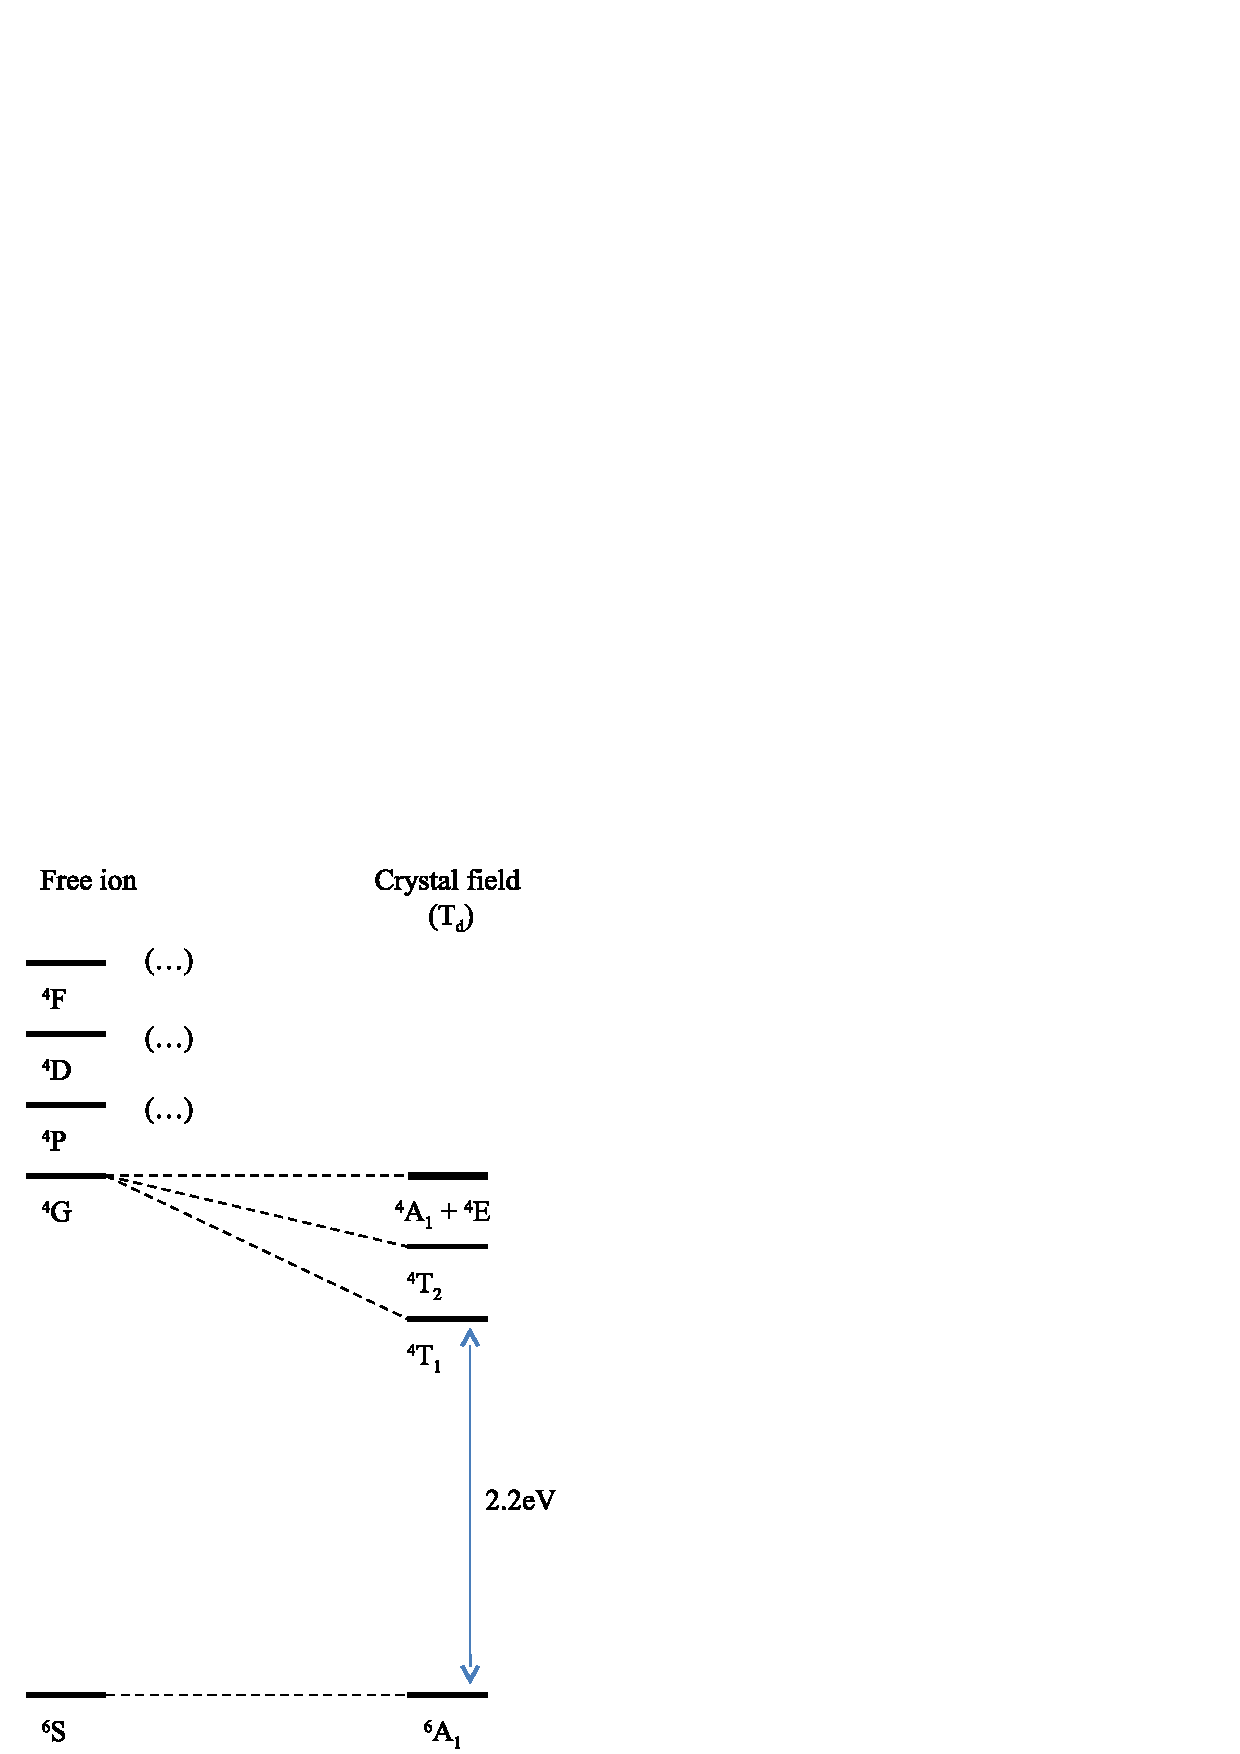
\includegraphics[width=10cm]{01-QD/Pictures/MnCrystal.png}
	\end{center}
	\caption{A schematic diagram of the splitting of the lowest excited states of the $3d^5$ level ($^4$G) relative to the ground state ($^6$S) for a Mn$^{2+}$ ion in the presence of a tetrahedral crystal field.}
	\label{MnCrystal}
	\end{figure}
		
		The interaction with the crystal field will lift the degeneracies of the free atom level. Those new levels are written with the appropriate group theoritical transformation properties. The $^6$S ground state is symmetrical and non-degenrated. Thus, in first order, it is not affected by the crystal field and is noted $^6$A$_1$. On the other hand, $^4$G, the first excited state, is degenerated and therefore is affected by the crystal. It split into four different states: $^4$T$_1$, three-fold degenerated ; $^4$T$_2$, three-fold degenerated ; $^4$E, two-fold degenerated ; and $^4$A$_1$, not degenerated. It has been shown by calculations that the effect of the crystal field is to pull the two $^4$T levels closer to the ground state, while $^4$E and $^4$A$_1$ are almost coincident and almost not affected by the crystal field~\cite{TanabeGroupThMn,SolidStatesPhysics,ThTransMetalIon}. Higher energy excited states would also be affected, but they are at high enough energy for their contribution not to be significant.

	For a free atom, the transition between the ground state with $S=\frac{5}{2}$ and any of the excited state, with $S = \frac{3}{2}$ is forbidden by the $\Delta S = 0$ rule and the parity selection ones. However, in a II-VI lattice, the spin-orbit interaction and the absence of inversion symmetry relax those rules, and thus allow the transitions between $^6$A$_1$ and the different states coming from the $^4$G splitting. $^6$A$_1 \rightarrow ^4$T$_1$ is the lowest energy of those transitions and therefore the most significant. It corresponds to approximately 2.2 eV. This transition can kill the luminescence of a semiconductor: the electron-hole recombination excite the Mn transition, flipping a d electron instead of emitting a photon. However, this transition is unlikely to happen. To have a significant effect on the luminescence, we need a semiconductor with a gap wider than the energy needed for the transition and a high concentration of Mn atom. CdTe have a bandgap of 1.6 eV at 5K~\cite{FurdynaDMS}, although it can be widened by the confinement of the QD, and we work at a really low concentration of Mn atoms in order to have QD with only one of them. This phenomena shouldn't then have a noticeable effect on our samples.
	

	$^6$A state of the Mn$^{2+}$ is symmetric and thus not affected by the crystal field nor the biaxial strain. 
However, inserting the Mn in a lattice affect its exterior orbital through the spin-orbit coupling. This interaction is mainly driven by the anisotropy of strain, splitting the spin level according to $D_0S_z^2$, with $D_0$ the magnetic anisotropy and $S_z$ the Mn spin quantified along the $z$ axis. The Mn nuclear spin $I = \frac{5}{2}$ also couple to its electronic spin, giving to the atom an hyperfine structure. The whole hamiltonian of an electronic spin coupled to the nuclear spin of a Mn atom in a strained layer grow along [001] axis is known from electron paramagnetic resonance in CdTe/ZnTe superlattices~\cite{StrainedMn} and reads:
	\begin{align}
	\label{Mnalone}
		\begin{array}{rll}
			{\cal H}_{Mn} &=& {\cal A}\mathbf{I}.\mathbf{S} \\
							& & +\dfrac{1}{6}a (S_x^4 + S_y^4 + S_z^4 - \dfrac{1}{5}S(S+1)(3S^2+3S-1)) \\
							& & + D_0 (S_z^2 - \dfrac{1}{3}S(S+1)) + E(S_x^2 - S_y^2)
		\end{array}
	\end{align}
	
	\begin{figure}[h!]
	\begin{center}
		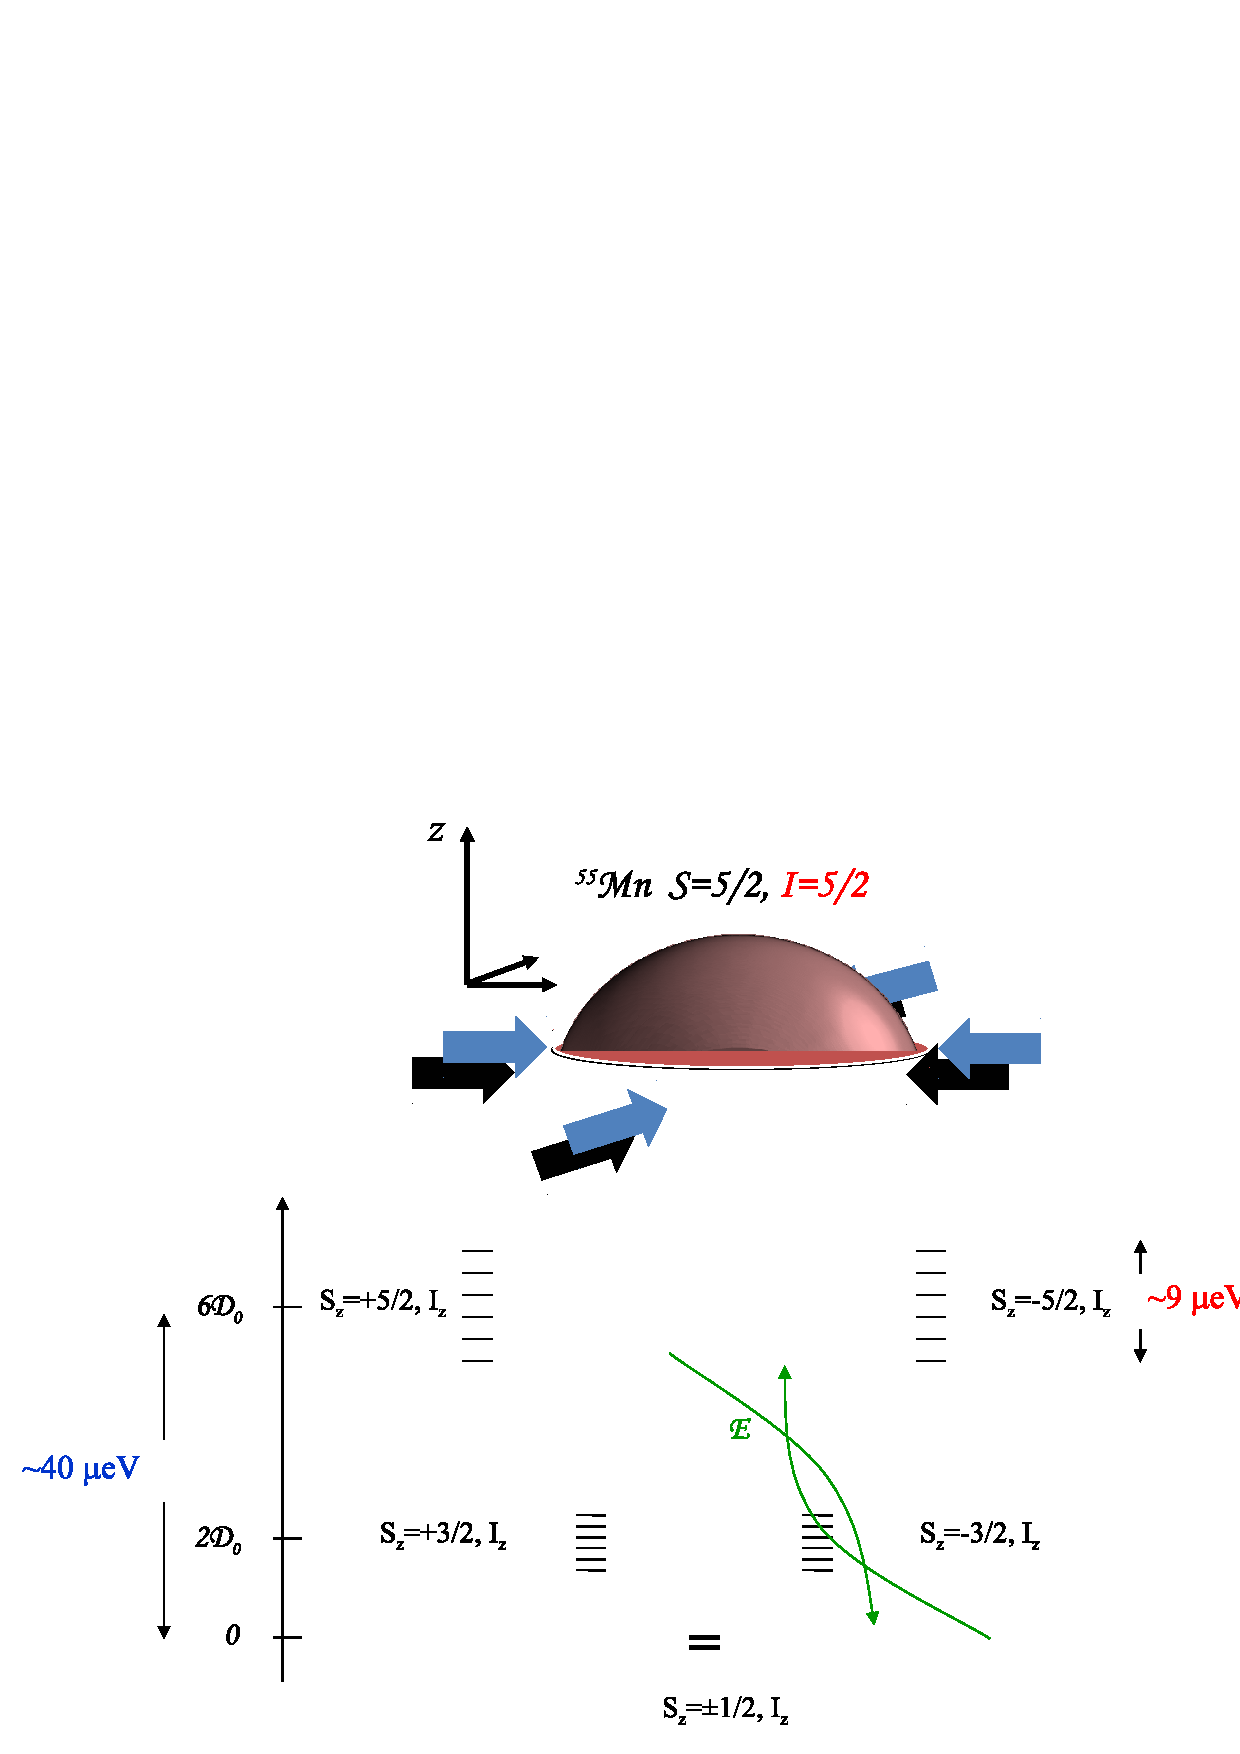
\includegraphics[width=12cm]{01-QD/Pictures/MnFineStruct.png}
	\end{center}
	\caption{Top: picture of an idealized strained QD containing a magnetic atom. Bottom: scheme of the energy level of a Mn atom in a strained II-VI QD. All the stable Mn isotopes $^{55}$Mn carries a nuclear spin $I = \frac{5}{2}$ which couples through the hyperfine interaction (${\cal A}\mathbf{I}.\mathbf{S}$) to the electronic spin $S = \frac{5}{2}$.The $d$ orbital of the Mn is also sensitive to the electric field produced by the neighbouring crystal atoms (crystal field) in the zinc-blend lattice. A distortion of the lattice and consequently a change in the crystal field will also affect the $d$ orbital. The dynamic of the Mn spin at zero magnetic field is mainly controlled by a magnetic anisotropy $D_0$ produced by the presence of a large bi-axial strain at the Mn location. This field splits the spin states of the Mn according to $D_0 S_z^2$; the anisotropy of the strain in the quantum dot plane ($E(S_x^2 - S_y^2)$) also mix the different $S_z$ component (green arrow).}
	\label{MnFineHyperfines}
	\end{figure}
	
	The first term is the hyperfine interaction between the Mn nuclear spin $\mathbf{I}$ and its $5d$ electrons spin $\mathbf{S}$, coupling two consecutive Mn spin states through an electron-nuclei flip flop. The hyperfine constant of the Mn was found to be ${\cal A} \approx 0.71$ $\mu$eV~\cite{MnSpinLatticeCoeff}. The second term results from the crystal cubic symmetry and mixes different $S_z$ of the Mn spin. According to ref.~\cite{MnSpinLatticeCoeff}, we have $a = 0.32$ $\mu$eV.
	
	The last line contains terms linked to the strain state at the Mn position: the magnetic anisotropy caused by bi-axial strain $D_0$ and the anisotropy of strain in the $xy$ plane $E$. Because of the partial relaxation of strain in the self-assembled QD we used, the value of $D_0$ may vary between 0 $\mu$eV for a strain-free QD, to 12 $\mu$eV for a fully strain CdTe layer matched on ZnTe. Typical values around 7 $\mu$eV are usually observed in CdTe/ZnTe QDs~\cite{MnResSpinDyn,GorycaPrecession}, leading to the 40 $\mu$eV splitting presented on Fig.~\ref{MnFineHyperfines}. It is responsible for the Mn spin memory at zero magnetic field~\cite{ClaireOptSpinOr}.
	
	The anisotropy in the QD plane induces a mixing between different $S_z$ through the anisotropic crystal field component $E$. It coupled two values of $S_z$ separated by two units of spin. In the absence of magnetic anisotropy ($D_0 \simeq 0$), both the anisotropy of strain and the hyperfine structure prevent the optical pumping of the Mn spin at 0 magnetic field.

		\subsection{Cr atom in II-VI semiconductor\label{CrSemiCon}}
	
		

		Cr atoms are incorporated into II-VI semiconductors as Cr$^{2+}$ ions on cation sites forming a deep impurity level. 90\% of Cr isotopes presents \emph{no nuclear spin}, meaning we do not have to consider their hyperfine structure in II-VI semiconductors. The ground state of a free Cr$^{2+}$ is $^{5}$D with the orbital quantum number L=2 and a spin S=2 yielding a 25-fold degeneracy. In the crystal field of T$_{d}$ symmetry of the tetrahedral cation site in zinc-blende crystal, the degeneracy is partially lifted (see Fig.~\ref{CrinIIVI}): the $^{5}$D term splits into 15-fold degenerate orbital triplet $^{5}$T$_{2}$ and 10-fold degenerate orbital doublet $^{5}$E. The Jahn-Teller distortion reduces the symmetry to D$_{2d}$ and leads to a splitting of the $^{5}$T$_{2}$ ground state into a 5-fold degenerate $^{5}$B$_{2}$ orbital singlet and a $^{5}$E orbital doublet .

		The ground state orbital singlet $^{5}$B$_{2}$ is further split by the spin-orbit interaction. In a strain free crystal, it was found that the ground state splitting can be described by the spin effective Hamiltonian~\cite{EPRCr}:
		\begin{align}
			\label{exchange}
			{\cal H}_{Cr,CF}=D_0S_z^2+\frac{1}{180}F[35S_z^2-30S(S+1)S_z^2+25S_z^2]+\frac{1}{6}a[S_1^4+S_2^4+S_3^4]
		\end{align}
with the Cr spin $S=2$ and $|D_0|\gg|a|$, $|F|$. In the model presented here, we use $a=0$ and $F=0$. The x, y, z principal axes were found to coincide with the cubic axes (1,2,3) giving rise to three identical sites, each given by \ref{exchange} but with the z axis of each along a different cubic axis (1,2,3). A value of $D_0\approx+30$ $\mu$eV was estimated from Electron Paramagnetic Resonance (EPR) measurements in highly diluted bulk (Cd,Cr)Te~\cite{EPRCr}.

		\begin{figure}[hbt]
			\label{CrinIIVI}
			\begin{center}
				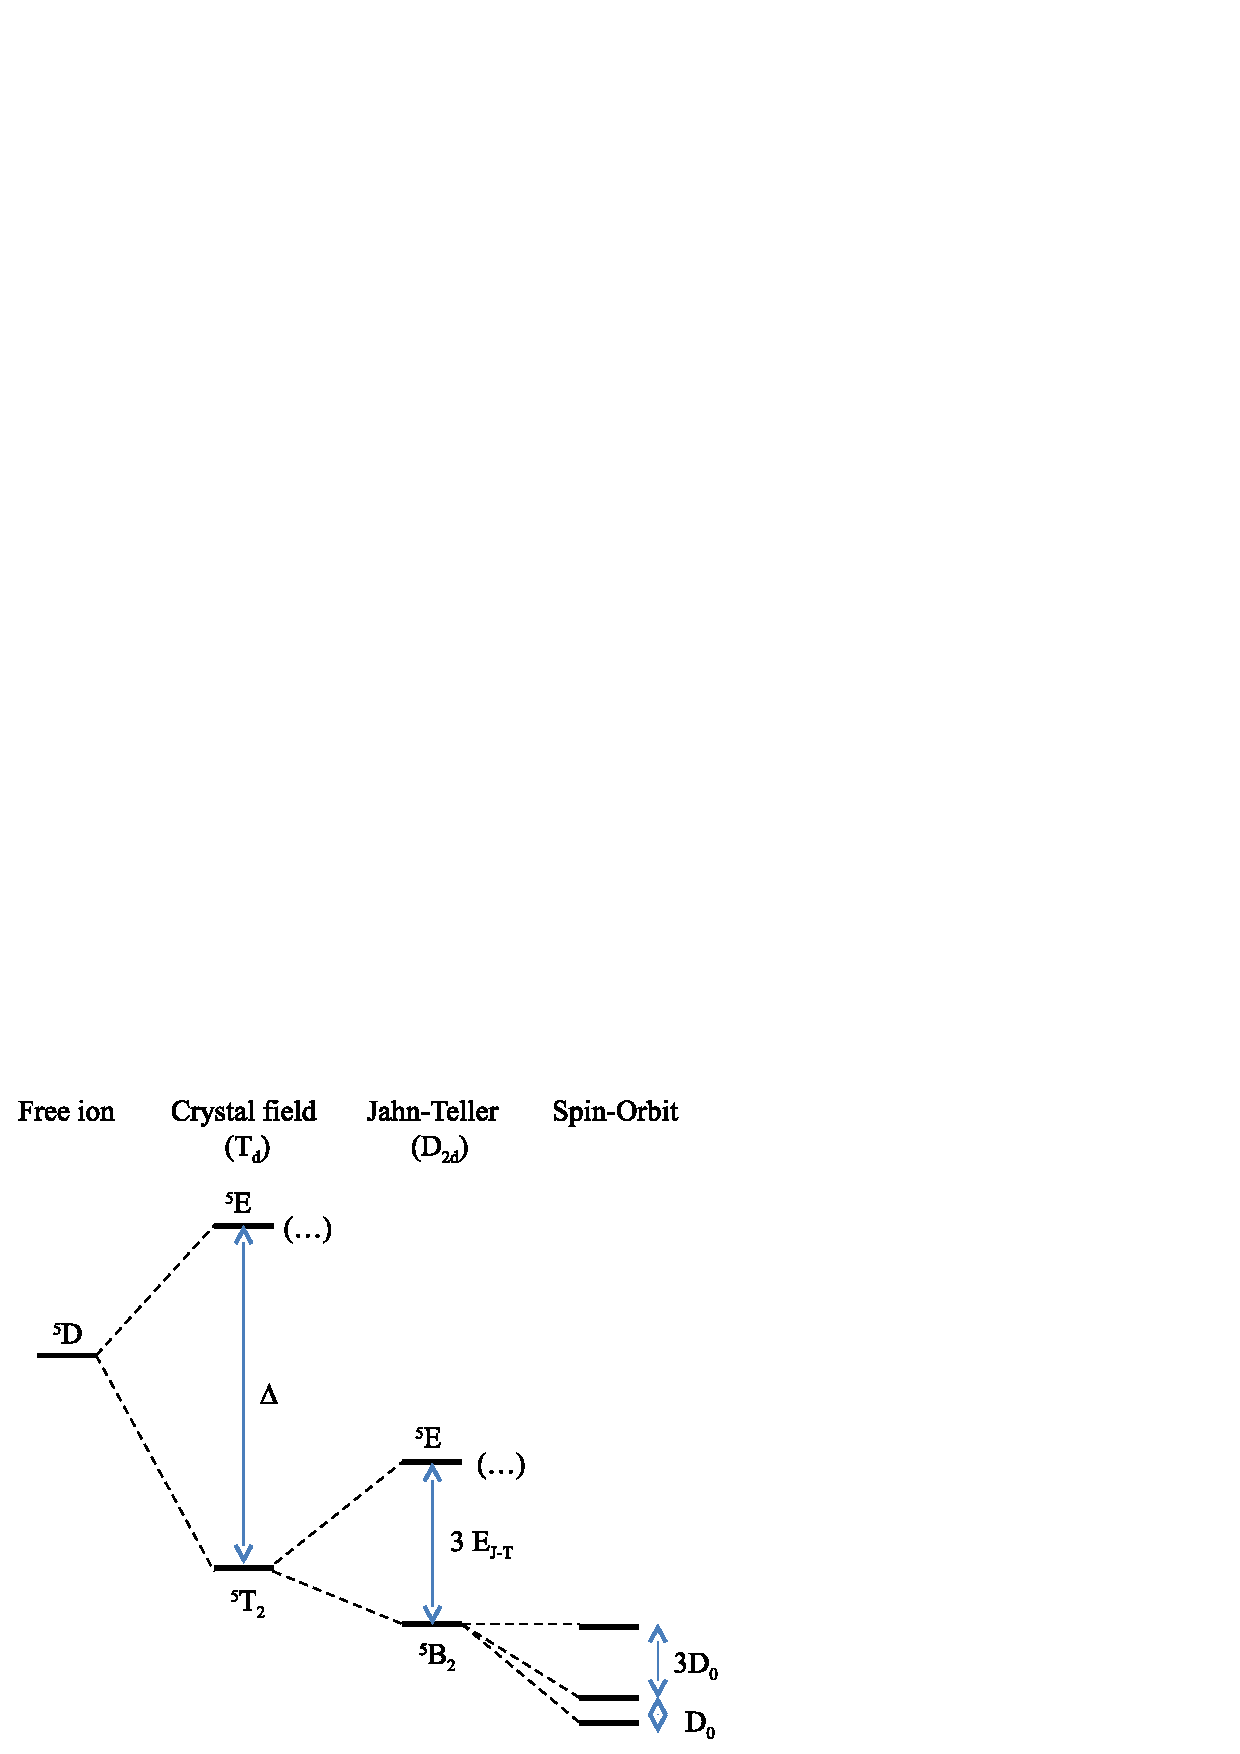
\includegraphics[width=10cm]{01-QD/Pictures/CrinIIVI.png}
			\end{center}
			\caption{Schema of the energy level splitting of Cr$^{2+}$ at a cation site in II-VI compounds having zinc blende structure (T$_d$) with a crystal field parameter $\Delta$, a Jahn-Teller energy $E_{J-T}$ and a spin-orbit level spacing $D_0$.}
		\end{figure}

		Static biaxial compressive strain in the (001) plane, as observed in self-assembled quantum dots, reduces the symmetry to D$_{2d}$ and destabilize the Cr $3d$ orbitals $d_{xz}$ and $d_{yz}$ having an electron density pointing along the $[$001$]$ axis ($z$ axis). The Cr ground state is then a 5-fold degenerated orbital singlet formed from the $d_{xy}$ orbital. It corresponds to the Jahn-Teller ground state with a tetragonal distortion along the $[$001$]$ axis~\cite{DefPonctSemiCon}.

		An applied stress will also  influence the Cr spin fine structure splitting through the modification of the crystal field and the spin-orbit interaction~\cite{EPRCr}. For an arbitrary strain tensor, the general form of the Cr ground state spin effective Hamiltonian is
		\begin{align}
		\label{FullCrHamil}
			{\cal H}_{Cr,\varepsilon} = c_1 e_A S_{\theta} + c_2 e_{\theta} S_{\theta} + c_3 e_{\epsilon} S_{\epsilon} + c_4e_{\zeta} S_{\zeta} + c_5(e_{\xi} S_{\xi} + e_{\eta} S_{\eta})
		\end{align}
with $S_i$ defined as:
		\begin{align}
			\begin{array}{rl}
			\label{Svalues}
				S_{\theta} &= S_{z}^2  -\dfrac{1}{2} [S_{x}^2 + S_{y}^2] \\
				S_{\epsilon} &= \dfrac{1}{2} \sqrt{3} [S_{x}^2 - S_{y}^2] \\
				S_{\xi} &= S_{y} S_{z} + S_{z} S_{y} \\
				S_{\eta} & = S_{x} S_{z} + S_{z} S_{x} \\
				S_{\zeta} &=S_{x} S_{y} + S_{y} S_{x}
			\end{array}
		\end{align}
and $e_i$ defined similarly as:
		\begin{align}
			\begin{array}{rl}
			\label{evalues}
				e_{\theta} &= \varepsilon_{zz} - \dfrac{1}{2} [\varepsilon_{xx} + \varepsilon_{yy}] \\
				e_{\epsilon} &= \dfrac{1}{2} \sqrt{3}[\varepsilon_{xx} - \varepsilon_{yy}] \\
				e_{\xi} &= \varepsilon_{yz} + \varepsilon_{zy} \\
				e_{\eta} &= \varepsilon_{xz} + \varepsilon_{zx} \\
				e_{\zeta} &= \varepsilon_{xy} + \varepsilon_{yx} \\
				e_A &= \varepsilon_{xx} + \varepsilon_{yy} + \varepsilon_{zz}			
			\end{array}
		\end{align}

		As shown in Sec.~\ref{BPSec}, we can write for a flat self-assembled quantum dot with dominant large biaxial strain:
		\begin{align*}
			\varepsilon_{xx} = \varepsilon_{yy} = \varepsilon_{\parallel} \\
			\varepsilon_{zz}=-2\frac{C_{11}}{C_{12}}\varepsilon_{\parallel}
		\end{align*}
where C$_{11}\approx$ 5.4 10$^{10}$ Pa and C$_{12}\approx$ 3.7 10$^{10}$ Pa are the elastic constants of CdTe~\cite{CdTeElConst}. For this strain configuration, the Cr fine structure is controlled by the spin-lattice coupling coefficients $c_1$ (symmetric coefficient) and $c_2$ (tetragonal coefficients). Strain-coupling coefficients estimated from EPR measurements in bulk Cr doped CdTe are listed in table \ref{StrCouplCoef}.

		\begin{table}[htb] \centering
			\caption{Values for spin to strain coupling coefficients of Cr in bulk CdTe (in $meV$) extracted from ref.~\cite{EPRCr}.\label{StrCouplCoef}}
			\renewcommand{\arraystretch}{1.0}
			\begin{tabular}{ccccc}
				\hline\hline
				$c_{1}$ & $c_{2}$ & $c_{3}$  & $c_{4}$  & $c_{5}$ \\
				-0.25$\pm$2 & +4.9 $\pm$2& -1.25$\pm$0.5 & +4.9$\pm$2 & +3.7$\pm$1.25 \\
				\hline\hline
			\end{tabular}
		\end{table}

		We can now simplify the hamiltonian \ref{FullCrHamil}, first reducing it to the active term in our case:
		\begin{align*}
			{\cal H}_{Cr,\varepsilon} &= c_1 e_A S_{\theta} + c_2 e_{\theta} S_{\theta}
		\end{align*}
Replacing now $e_A$, $e_{\theta}$ and $S_{\theta}$ by their value given in \ref{Svalues} and \ref{evalues}, and using the equalities given in Sec.~\ref{BPSec}, we can rewrite the strain controlled part of the spin Hamiltonian as ${\cal H}_{Cr,\varepsilon}$, depending only on $\varepsilon_{\parallel}$:
		\begin{align}
			\begin{array}{rlcc}
			\label{HamilD0}
				{\cal H}_{Cr,\varepsilon_{\parallel}} &=& \underbrace{\dfrac{3}{2}\varepsilon_{\parallel}[2c_1(1-\dfrac{C_{12}}{C_{11}})-c_2(1+2\dfrac{C_{12}}{C_{11}})]} & S_z^2 \\
													&=& D_0 & S_z^2
			\end{array}
		\end{align}
where we can estimate $D_0\approx 1\pm0.6$ meV from the values of the spin-strain coupling coefficients in CdTe (table \ref{StrCouplCoef}). This is about 100 times stronger than the value found in Mn quantums dots, as stated on Sec.~\ref{MnSemiCon}.
However one should note the quantum dots could be partially relaxed and may contain a significant amount of Zn. This can significantly change the spin-strain coupling coefficients of the Cr atom.

		An anisotropy of the strain in the quantum dot plane (001) with principal axis along $[$010$]$ or $[$100$]$ axes ($\varepsilon_{xx}\neq\varepsilon_{yy}$ and $\varepsilon_{xy} = \varepsilon_{yx}=0$) would affect the Cr fine structure through the tetragonal coefficient $c_3$. This coupling can be described by an additional term in the spin-strain Hamiltonian
		\begin{align}
			\begin{array}{rlcc}
			\label{HamilE}
				{\cal H}_{Cr,\varepsilon_{\perp}} &=& \underbrace{\dfrac{3}{4} c_3 (\varepsilon_{xx}-\varepsilon_{yy})} & (S_x^2 - S_y^2) \\
												&=& E & (S_x^2 - S_y^2)
			\end{array}
		\end{align}

		This anisotropy term $E$ couples Cr spin states separated by two units and in particular $S_z$=+1 to $S_z$=-1 which are initially degenerated. It could be exploited to induce a large strain mediated coherent coupling between a mechanical oscillator and the Cr spin~\cite{SpinOsciCoupl}.
		
		We can now group \ref{HamilD0} and \ref{HamilE} in order to write the complete hamiltonian of an isolated Cr in a strained, anisotropic CdTe/ZnTe quantum dot:
		\begin{align}
			\begin{array}{lrccc}
				\label{Cralone}
				{\cal H}_{Cr,\varepsilon} &=& {\cal H}_{Cr,\varepsilon_{\parallel}} &+& {\cal H}_{Cr,\varepsilon_{\perp}} \\
										&=& D_0 S_z^2 &+& E(S_y^2 - S_x^2)
			\end{array}
		\end{align}
		
		This strong coupling to strain make the Cr a choice element for spin-mechanical system. This control can be achieved with surface accoustic waves (SAW). Plans are done to deposit on the surface of the sample piezzo-electric material in order to induce SAW along the the $xy$ axis. We can then externally generate in-plane strain to control the Cr spin.
	
	
	\section{A simple example: the X-Mn system}
	
	In order to illustrate the concepts explained in this chapter, we will do a quick study of a well known system: the exciton coupled to a single Manganese atom. In order to simplify the study, let's consider a QD containing a single Mn atom with no shape or strain anisotropy. When an exciton is injected in, it will interact with the magnetic atom on top of the hole-electron interaction already taking place for an exciton. The hamiltonian of the system reads:
	\begin{align}
		\label{HXMn}
		{\cal H}_{XMn} = {\cal H}_{eh} + {\cal H}_{eMn} + {\cal H}_{hMn}
	\end{align}
We use in this part the heavy-hole approximation, ignoring the effect of the non-diagonal term of the band hamiltonian. In order to simplify the notation, we write $|S_{z, Mn}\rangle = |S_z\rangle$.

	\begin{figure}[h!]
	\begin{center}
		\includegraphics[width=11cm]{01-QD/Pictures/XMn-Exp.eps}
	\end{center}
	\caption{Photoluminescence of the X, X$^-$ and X$^2$ complex for (a) a undoped QD and (b) a QD containing a single Mn atom.}
	\label{MnSpectra}
	\end{figure}

	In the heavy hole subspace, in the $\sigma_z$, $j_z$, $S_z$ basis, all the hamiltonians describing an interaction with the hole are diagonal. Therefore, the only non-diagonal element in the hamiltonian~\ref{HXMn} describe electron-Mn spin-flips. The hole having no part in this interaction, those spin-flips couple a bright state to a dark state, separated by $\delta_0$, as defined in Sec.~\ref{ehExch}. The strength of this interaction is of the same magnitude of $I_{eMn}$, found to be in the 100 $\mu$eV range in our quantum dots~\cite{DynhMn}. The distance between the bright and dark states is then about one order of magnitude higher than the strength of the interaction. We can thus neglect it.
	
	We can now consider the hamiltonian~\ref{HXMn} to be diagonal. The interaction of the Mn spin with electron is ferromagnetic with $I_{eMn} \simeq -100$ $\mu$eV, while its interaction with the hole is anti-ferromagnetic with $I_{hMn} \simeq 250$ $\mu$eV.  The carriers act as an effective magnetic field along the growth axis. This lift the degeneracy of the Mn spins in a sextuplet. For the bright exciton, with anti-parallel spins, the lift is the strongest. Each Mn spin state is separated from the closest one by $\frac{1}{2}(3I_{hMn} - I_{eMn})$, for a total energy span of $\frac{5}{2}(3I_{hMn} - I_{eMn})$. For the dark exciton states, each of them are separated from the closest one by $\frac{1}{2}(3I_{hMn} + I_{eMn})$, for total energy span of $\frac{5}{2}(3I_{hMn} + I_{eMn})$. The bright and dark excitons are splitted by the electron-hole exchange interaction $I_{eh} \simeq 750$ $\mu$eV. All these splitting are a lot larger than the one induced by the crystal field and the hyperfine structure.
	
	One can note that the system is symmetric under inversion of the quantification axis $z$. Excitons with opposed spins coupled to opposed Mn spins will then be degenerated. For instance, $|S_z = \frac{5}{2}, X_z = -1\rangle$ share the same energy level as $|S_z = -\frac{5}{2}, X_z = +1\rangle$. The whole energy level structure is summarize in Fig.~\ref{MnLevel}.

	\begin{figure}[h!]
	\begin{center}
		\includegraphics[width=12cm]{01-QD/Pictures/MnEnLvl.png}
	\end{center}
	\caption{Energy level of the ground state and the exciton in a Mn-doped QD. The levels are sketched as a function of the Mn spin $S_z$. Dark states are represented in grey. Optical transitions from the bright states of the Mn complex results in six-line PL spectra, such as in Fig.~\ref{MnSpectra}.}
	\label{MnLevel}
	\end{figure}
	
	The fundamental state of the QD is an isolated Mn atom in the dot. In our QDs, we usually find $D_0 \simeq 7$ $\mu$eV~\cite{MnResSpinDyn,GorycaPrecession}, negligible compared to the exciton-Mn interactions. Since the other fine structure parameters of the Mn are less intense than $D_0$, we choose to neglect their contribution to the spectra. Therefore, the fundamental state of the QD is six time degenerated. The recombination does not affect the Mn spin. Each emission line is thus the superposition of two optical transitions with opposed circular polarization (recombination of an excition $X_z = \pm1$). In a given polarization, each line corresponds then to a single Mn spin: the spectra is a photography of the statistic state of the Mn spin during the exciton recombination.

	
	This simple model is however incomplete. More thorough investigation of the system were done in \cite{YoanTh}. The effects of the VBM, and the strain and shape anisotropy on the system was studied in \cite{DELum}. A complete study of the dynamic of the system was done by Claire Le Gall in her PhD thesis~\cite{ClaireTh}.
	





\chapter{Growth of the samples\label{Growth}}

	

	\section{Strained dots: CdTe/ZnTE\label{SK}}
	
	\subsection{Substrate preparation}
	
	\subsection{Strained dots growth\label{SKGrowth}}
	
	\section{Other kind of samples}
		\subsection{Charge control samples}	
		
	
		\subsection{Strain-free quantum dots\label{SFD}}


\chapter{Coherent dynamics of Mn-doped positively charged quantum dots}

	\section{Mn in a II-VI positively charged quantum dot}
		
		\subsection{Spin structure of a positively charged Mn doped quantum dot}
		
	\lipsum[1]
		
	\begin{figure}[h!]
	{\caption{(a) Color scale plot of the PL intensity of the studied Mn doped QD inserted in Schottky structure showing the emission of the neutral (X-Mn) and positively charged (X$^+$-Mn) exciton as a function of energy and bias voltage. (b) PL of the Mn-doped QD under a positive bias voltage of V=5.5V.}\label{hMnspectra}}
	{\begin{center}
		\includegraphics[width=12cm]{03-h-Mn/Pictures/DotPres.eps}
	\end{center}}
	\end{figure}
	
	\lipsum[3-4]
		
	\begin{figure}[h!]
	\begin{center}
		\includegraphics[width=14.8cm]{03-h-Mn/Pictures/Recomb.png}
	\end{center}
	\caption{Electron-Mn spin states for each $|M,M_z\rangle$. For each $M$, the $\sigma-$ (red) and $\sigma+$ (blue) probability is highlighted. This probability is directly linked to the intensity of each peak. In the center, the different possible recombination path for $M=3$ and $M=2$ are presented. A schema of the resulting spectra is drawn below.}
	\label{Recomb}
	\end{figure}

	\lipsum[5]
	
	\begin{figure}[h!]
	\begin{center}
		\includegraphics[width=12cm]{03-h-Mn/Pictures/Spinstructv2.png}
	\end{center}
	\caption{(a) Energy levels of the ground (h-Mn) and excited ($X^+$-Mn) states as a function of their angular momentum (M$_z$). The levels in dotted lines corresponds to the h-Mn states $|-1/2\rangle|\Uparrow\rangle$ and $|+1/2\rangle|\Downarrow\rangle$ coupled by the valence band mixing. Optical recombination towards these levels leads to the linearly polarized lines observed in (b). (b) Experimental (left) and calculated (right) color-scale plot of the linear polarization dependence of the PL of X$^+$-Mn at B = 0 T (top) and B$_\perp$ = 0.42 T (bottom). The parameters used in the calculation are listed in Table~\ref{paraQD}.}
	\label{CompleteEnerStruct}
	\end{figure}
	
	\lipsum[7]
	
	\begin{table}[t] \centering
		\caption{Values of the parameters used in the model of the positively charged Mn-doped QD presented in Fig.~\ref{hMnspectra}. I$_{eMn}$, I$_{hMn}$, $\frac{\rho_s}{\Delta_{lh}}$, $\theta$, $\eta$ and $T_{eff}$ are used to model the linear polarization intensity map of Fig.~\ref{CompleteEnerStruct}. The other parameters cannot be extracted from the PL measurements and values for typical Mn-doped QDs are chosen for the calculation of the spin dynamics presented in Sec.~\ref{SpinDyn} and \ref{StrainInfl}.}
		\begin{tabular}{cccccc|ccccc}
			\hline\hline
			I$_{eMn}$ & I$_{hMn}$ & $\frac{\rho_s}{\Delta_{lh}}$ & $\theta$    & $\eta$   & $T_{eff}$  & $g_{e}$ & $g_{h}$   	& $g_{Mn}$ & $D_0$    &  $E$      \\
			$\mu eV$  & $\mu eV$  &                              & $^{\circ}$  & $\mu eV$ &    K       &         &           &          & $\mu eV$ &  $\mu eV$ \\
			\hline
			-175    &     345   &        0.09                  &    0        &     30   &   20       &  -0,4   &  0.6      &     2    &    7     &   1.5     \\
			\hline\hline
		\end{tabular}
		\label{paraQD}
	\end{table}
	

		\subsection{Optical $\Lambda$-level identification\label{LambdaId}}	
		
		\lipsum[11]
	
	\begin{figure}[h!]
	\begin{center}
		\includegraphics[width=12cm]{03-h-Mn/Pictures/Lambdasyst.png}
	\end{center}
	\caption{(a) Non resonant (Non Res.) and resonant (Res.) PL of X$^+$-Mn. Co and cross circularly polarized PL spectra are collected for three different energies of the CW resonant laser (green). Inset: intensity map of the cross-circularly polarized PL detected on the low energy side of X$^+$-Mn as the CW laser is scanned through the high energy side. (b) Energy levels of X$^+$-Mn and identification of the three resonances observed in (a) corresponding to the optical $\Lambda$ systems associated with the e-Mn states $|3,+1\rangle$, $|3,+2\rangle$ and $|2,+2\rangle$.}
	\label{LambdaLevel}
	\end{figure}
	
	\lipsum[12]
			
	
	\section{Spin dynamics under resonant excitation\label{SpinDyn}}
	
	
		\subsection{Cycling and escaping the $\lambda$-level system}


\lipsum[5-6]
	
	\begin{figure}[h!]
	\begin{center}
		\includegraphics[width=14.8cm]{03-h-Mn/Pictures/ResAutocor.eps}
	\end{center}
	\caption{Auto-correlation of the resonant PL for cross-circularly polarized excitation and detection of the electron-Mn states (a) $|3, +1\rangle$, (b) $|3, +2\rangle$ and (c) $|2, +2\rangle$.}
	\label{AllAutocorB0}
	\end{figure}
	
\lipsum[7-8]
	
	\begin{figure}[h!]
	\fcapside{\caption{Schema of the energy levels of the optical $\Lambda$ system associated with the electron-Mn state $|3, +2\rangle$ extracted from the full level structure of a positively charged Mn-doped QD (Fig.~\ref{LambdaLevel}). The different processes discussed in this section are presented on it.}\label{LambdLoop}}	
	{\begin{center}
		\includegraphics[width=6cm]{03-h-Mn/Pictures/RelaxMecanism.png}
	\end{center}}
	\end{figure}

\lipsum[9]
	
		\begin{figure}[h!]
			\begin{center}
				\includegraphics[width=12cm]{03-h-Mn/Pictures/AutocorBPw.eps}
			\end{center}
			\caption{Excitation power dependence (a) and transverse magnetic field dependence (b) of the auto-correlation of the resonant PL obtained for an excitation on the high energy branch of the $\Lambda$ level system associated to the e-Mn state $|2,+2\rangle$.}
			\label{AutocorExpBPw}
		\end{figure}
	
\lipsum[10-11]

	\begin{figure}[h!]
	\begin{center}
		\includegraphics[width=14.7cm]{03-h-Mn/Pictures/ResPumpv2.png}
	\end{center}
	\caption{Resonant optical pumping transients obtained under circular polarization switching of the resonant excitation for the $\Lambda$ systems associated with (a) $|3, +1\rangle$, (b) $|3, +2\rangle$ and (c) $|2, +2\rangle$ at zero field and under a weak longitudinal magnetic field B$_z$=0.23T. The insets present the corresponding states which are resonantly excited and detected in $\sigma-$ polarization.}
	\label{AllPumpB0}
	\end{figure}
	
\lipsum[12-13]

	\begin{figure}[h!]
	\begin{center}
		\includegraphics[width=12cm]{03-h-Mn/Pictures/PumpBPw.eps}
	\end{center}
	\caption{Excitation power dependence (a) and transverse magnetic field dependence (b) of the optical pumping signal obtained for a resonant excitation on $|3,+2\rangle$. Insets: excitation power dependence of the pumping time and transverse magnetic field dependence of the difference of resonant PL intensity between a $\sigma_{cross}$ and a $\sigma_{co}$ excitation.}
	\label{PumpExpBPw}
	\end{figure}
	
\lipsum[12-13]
	
	\begin{figure}[h!]
	\begin{center}
		\includegraphics[width=13cm]{03-h-Mn/Pictures/DarkRelax.png}
	\end{center}
	\caption{Optical pumping experiment for an excitation of $|3,+2\rangle$ with modulated circular polarization. A dark time ($\tau_{dark} = 50ns$) is introduced in the pumping sequence. The polarization switching occurs either before (black) or during (red) the dark time. The black and red diagrams present the corresponding resonant excitation sequences. The inset presents the variation of the ratio $\Delta I/I$ as a function of $\tau_{dark}$. The solid line is an exponential fit with $\tau_{relax} = 80 ns$.}
	\label{PumpExpDark}
	\end{figure}
	
\lipsum[12-14]
	
		\subsection{Relaxation mechanism\label{RelaxMech}}
	
			\subsubsection*{Hole-Mn flip-flops mediated by a lattice deformation}		
		
\lipsum[12-14]

		\begin{table}[hbt] \centering
			\caption{Material (CdTe or ZnTe) \cite{CdTeBPCoef} and QD parameters used in the calculation of the coupled hole and Mn spin relaxation time.}
			\begin{tabular}{lcr}
				\hline\hline
				CdTe& &\\
				\hline
				Deformation potential constants & b &  -1.0 eV  \\
												& d &  -4.4 eV  \\
				Longitudinal sound speed & c$_l$ &  3300 m/s  \\
				Transverse sound speed & c$_t$ &  1800 m/s  \\
				Density & $\rho$ &  5860 kg/m$^3$  \\
				\hline
				ZnTe& &\\
				\hline
				Deformation potential constants & b &  -1.4 eV  \\
												& d &  -4.4 eV  \\
				Longitudinal sound speed & c$_l$ &  3800 m/s  \\
				Transverse sound speed & c$_t$ &  2300 m/s  \\
				Density & $\rho$ &  5908 kg/m$^3$  \\
				\hline
				Quantum dot& &\\
				\hline
				Hole Mn exchange energy & I$_{hMn}$ &  0.35 meV  \\
				hh-lh exciton splitting&  $\Delta_{lh}$&  15 meV  \\
				Hole wave function widths: & &   \\
				- in plane & l$_{\bot}$ &3.0 nm   \\
				- z direction  & l$_z$ &1.25 nm   \\
				\hline\hline
			\end{tabular}
			\label{paraph}
		\end{table}

\lipsum[12]
	
	\begin{figure}[h!]
	\fcapside{\caption{Relaxation time $\tau_{ff}$, between the two Mn-hole ground states of the $\Lambda$ system  calculated with the material and QD parameters listed in Table \ref{paraph} and a temperature T=7K. The vertical line shows the energy splitting in the studied QD of the Mn-hole states involved in the $\Lambda$ systems considered here (Resonances (2) and (3) identified in Fig.~\ref{LambdaLevel}).}\label{TauRelax}}
	{\begin{center}
		\includegraphics[width=7cm]{03-h-Mn/Pictures/TauffRelax.eps}
	\end{center}}
	\end{figure}
	
\lipsum[12]
	
		\subsubsection*{Model of the carrier-Mn spin dynamics under resonant excitation}
	
\lipsum[12]

	\begin{figure}[h!]
	\begin{center}
		\includegraphics[width=10cm]{03-h-Mn/Pictures/AutocorSimu.eps}
	\end{center}
	\caption{(a) Calculated time evolution of $\rho_{|+\frac{3}{2},\uparrow_e\rangle}(t)$ with the QD parameters listed in Table~\ref{paraQD} and (unless specified) $\tau_r$=0.3ns, $\tau_{Mn}$=5 $\mu$s, $\tau_h$=10ns, $\tau_g$=0.25 ns, $\tau_{ff}$=1.5 ns, $T_2^{hMn}$= 5 ns, $T_2^{eMn}$= 0.5 ns, T=10K and B$_{\perp}$=0. (b) (c) and (d) illustrate the influence  of, respectively, $\tau_{ff}$, $\tau_g$ and $B_{\perp}$ on $\rho_{|+\frac{3}{2},\uparrow_e\rangle}(t)$. Note the different vertical scale in (b).}
	\label{AutocorModBPw}
	\end{figure}
	
\lipsum[12-13]

	\begin{figure}[h!]
	\begin{center}
		\includegraphics[width=12cm]{03-h-Mn/Pictures/PumpSimu.eps}
	\end{center}
	\caption{Calculated resonant optical pumping transients for a $\sigma-$ detection and an excitation of $|3,+2\rangle$ and $|3,-2\rangle$ with modulated circular polarization. The QD parameters for the calculations are those listed in table \ref{paraQD} and $\tau_r$=0.3 ns, $\tau_{Mn}$=5 $\mu$s, $\tau_h$=10 ns, $T_2^{hMn}$= 5 ns, $T_2^{eMn}$= 0.5 ns, $\tau_{ff}$=1.5 ns, T=10 K and $\tau_g$=0.25 ns. (a) Influence of a variation of $\tau_g$ and $\tau_{ff}$. (b) Influence of a transverse magnetic field $B_{\perp}$. The inset presents the transverse magnetic field dependence of the difference of population for a $\sigma+$ or a $\sigma-$ excitation.}
	\label{PumpModBPw}
	\end{figure}
	
\lipsum[12-13]
	
	\begin{figure}[h!]
	\begin{center}
		\includegraphics[width=13cm]{03-h-Mn/Pictures/RelaxDarkSimu.eps}
	\end{center}
	\caption{(a) Calculated time evolution in the dark of the population of the hole-Mn state $|+\frac{5}{2},\Downarrow_h\rangle$ initialized by a sequence of $\sigma-$/$\sigma+$ resonant excitation of $|3,-2\rangle$ and $|3,+2\rangle$. The dashed black line (shifted for clarity) is an exponential fit with a characteristic time $\tau_{relax}$=85 ns. (b) Corresponding calculated time evolution of the population $|+\frac{3}{2},\uparrow_e\rangle$. The parameters are those of Fig.~\ref{PumpModBPw}.}
	\label{PumpModDark}
	\end{figure}
	
\lipsum[12]

	\begin{figure}[h!]
	\begin{center}
		\includegraphics[width=12cm]{03-h-Mn/Pictures/StrainAutocorPump.eps}
	\end{center}
	\caption{(a) Calculated time evolution of $\rho_{|+\frac{1}{2},\uparrow_e\rangle}$ with $\rho_{|+\frac{1}{2},\Uparrow_h\rangle}$=1 (Mn-hole spin in the state $|+\frac{1}{2},\Uparrow_h\rangle$ after a $\sigma-$ recombination) for a resonant $\sigma+$ excitation of the coupled electron-Mn states $|3,+1\rangle$ and $|3,-1\rangle$ without and with a longitudinal magnetic field. (b) Time evolution of $\rho_{|+\frac{1}{2},\uparrow_e\rangle}$ under excitation with modulated circular polarization. The parameters used in the calculations are those of Fig.~\ref{PumpModBPw}.}
	\label{StrainAutocorPump}
	\end{figure}
	
\lipsum[12-13]

	\begin{figure}[h!]
	\caption{Energy levels of the ground (h-Mn) and excited ($X^+$-Mn) states as a function of their angular momentum (M$_z$). The e-Mn states $|3,+1\rangle$ and $|3,-1\rangle$, as well as $|2,+1\rangle$ and $|2,-1\rangle$, are coupled by the strain anisotropy $E(S_x^2-S_y^2)$. Optical $\Lambda$ systems associated with $|3,+1\rangle$ and $|3,-1\rangle$ are presented.}\label{LambdaMixed}
	{\begin{center}
		\includegraphics[width=9cm]{03-h-Mn/Pictures/SpinStructE.png}
	\end{center}}
	\end{figure}

	\section{Influence of the strain anisotropy\label{StrainInfl}}
	
	\begin{figure}[h!]
	\begin{center}
		\includegraphics[width=12.8cm]{03-h-Mn/Pictures/PolarRateTotal.eps}
	\end{center}
	\caption{(a) Configuration of the time resolved PL experiment for an excitation of $|3,+1\rangle$ (pulsed laser in green). (b) Top panel: Time resolved resonant PL of $|3,+1\rangle$ with a $\sigma+$/$\sigma-$ sequence of laser pulses and a detection in $\sigma+$ and $\sigma-$ polarization. Bottom panel: corresponding time dependence of the circular polarization rate $\kappa=(\sigma_{-}-\sigma_{+})/(\sigma_{-}+\sigma_{+})$. (c) Time dependence of the circular polarization rate of the resonant PL of the states $|3,+1\rangle$ (red), $|3,+2\rangle$ (black) and $|2,+2\rangle$ (blue). (d) Corresponding polarisation rates calculated with $D_0=7 \mu eV$~\cite{DynhMn}, $T_2^{eMn}=0.6ns$, $E=1.8\mu eV$, a radiative lifetime $T_r=0.3ns$ and the parameters listed on Tab.~\ref{paraQD}.}
	\label{PolarRateTotal}
	\end{figure}

		

	\begin{figure}[h!]
	\begin{center}
		\includegraphics[width=14cm]{03-h-Mn/Pictures/PolarRateB.png}
	\end{center}
	\caption{(a) Influence of a longitudinal (B$_z$, red) and a transverse (B$_x$, blue) magnetic field on the time dependence of the circular polarization rate $\kappa=(\sigma_{-}-\sigma_{+})/(\sigma_{-}+\sigma_{+})$ of the resonant PL of $|3,+1\rangle$, $|3,+2\rangle$ and $|2,+2\rangle$. On the top left panel, curves are shifted by 0.5 for clarity. (b) Corresponding time dependence of the circular polarization rate calculated with $g_{Mn}=2$, $g_{e}=-0.4$, $g_{h}=0.6$~\cite{DynhMn}, and the parameters listed on Table~\ref{paraQD}. The curves are shifted by 1 for clarity.}
	\label{hMnPolarRateB}
	\end{figure}
	
	\begin{figure}[h!]
	\begin{center}
		\includegraphics[width=11.2cm]{03-h-Mn/Pictures/LevelSplitB.eps}
	\end{center}
	\caption{(Color line) (a) Calculated energy of the electron-M, states in a longitudinal magnetic field (B$_z$) and in a transverse magnetic field (B$_{\bot}$). (b) Energy of the electron-Mn states for two orientations of the transverse magnetic field: $\phi = 0$ (B$_{\bot} = $ B$_x$) $\phi = \dfrac{\pi}{2}$ (B$_{\bot} = $ B$_y$). The parameters used in the calculations are listed in Table~\ref{paraph}, with the exception of $E$, for which the more precise value of 1.8 $\mu$eV was chosen.}
	\label{hMnPolarRateBMod}
	\end{figure}

\chapter{Magneto-optical study of Cr-doped CdTe quantum dots\label{MagOptStud}}


	The main goal of this thesis was to include single Cr atoms in CdTe/ZnTe QDs. It was successfully achieved. We saw in Sec.~\ref{CrSemiCon} how the Cr atom is incorporated in II-VI semiconductor. We will now optically study Cr-doped QDs in order to probe the carrier-Cr interactions.
	
	We begin presenting the photoluminescence (PL) and the energy structure of the X-Cr complex. It was sawn that the exchange interaction between the carrier and the Chromium is strong enough to see the effect of a single Cr spin in the quantum dots, giving the PL of the dots four characteristics peaks. We discuss the evolution of the emission in temperature and present different excited states of the system. Magneto-optical experiments confirm the energy structure, and hints at an anti-ferromagnetic between hole and Cr. In the next section, we use the evolution of the QDs PL under magnetic field in order to deduce the QD parameters, using a spin hamiltonian model including the strain induced fine structure of the magnetic atom, the exchange coupling with the carriers and the influence of the reduced symmetry of the QDs on the electron-hole exchange interaction and on the valence band. In the last section, we present dots having the characteristic four peaks PL, but that are not explained by our model. We finish proposing a possible explanation for those dots.


	\section{Strained quantum dots containing an individual X-Cr atom}
	
		\subsection{Energy structure of X-Cr in a quantum dot~\label{CrPres}}
		
		Using the procedure described in the 
		%Sec.~\ref{SKGrowth}
		Sec.~II.1, we randomly incorporated Cr atoms in CdTe/ZnTe quantum dots, adjusting the density of the Cr atoms to be roughly equal to the density of dots, in order to get QDs containing 0, 1 or a few Cr atoms. The photoluminescence (PL) of individual QDs, induced by optical excitation with a dye laser tuned on resonance with an excited state of the dots, is studied by optical micro-spectroscopy.
		
	\begin{figure}[h!]
	\begin{center}
		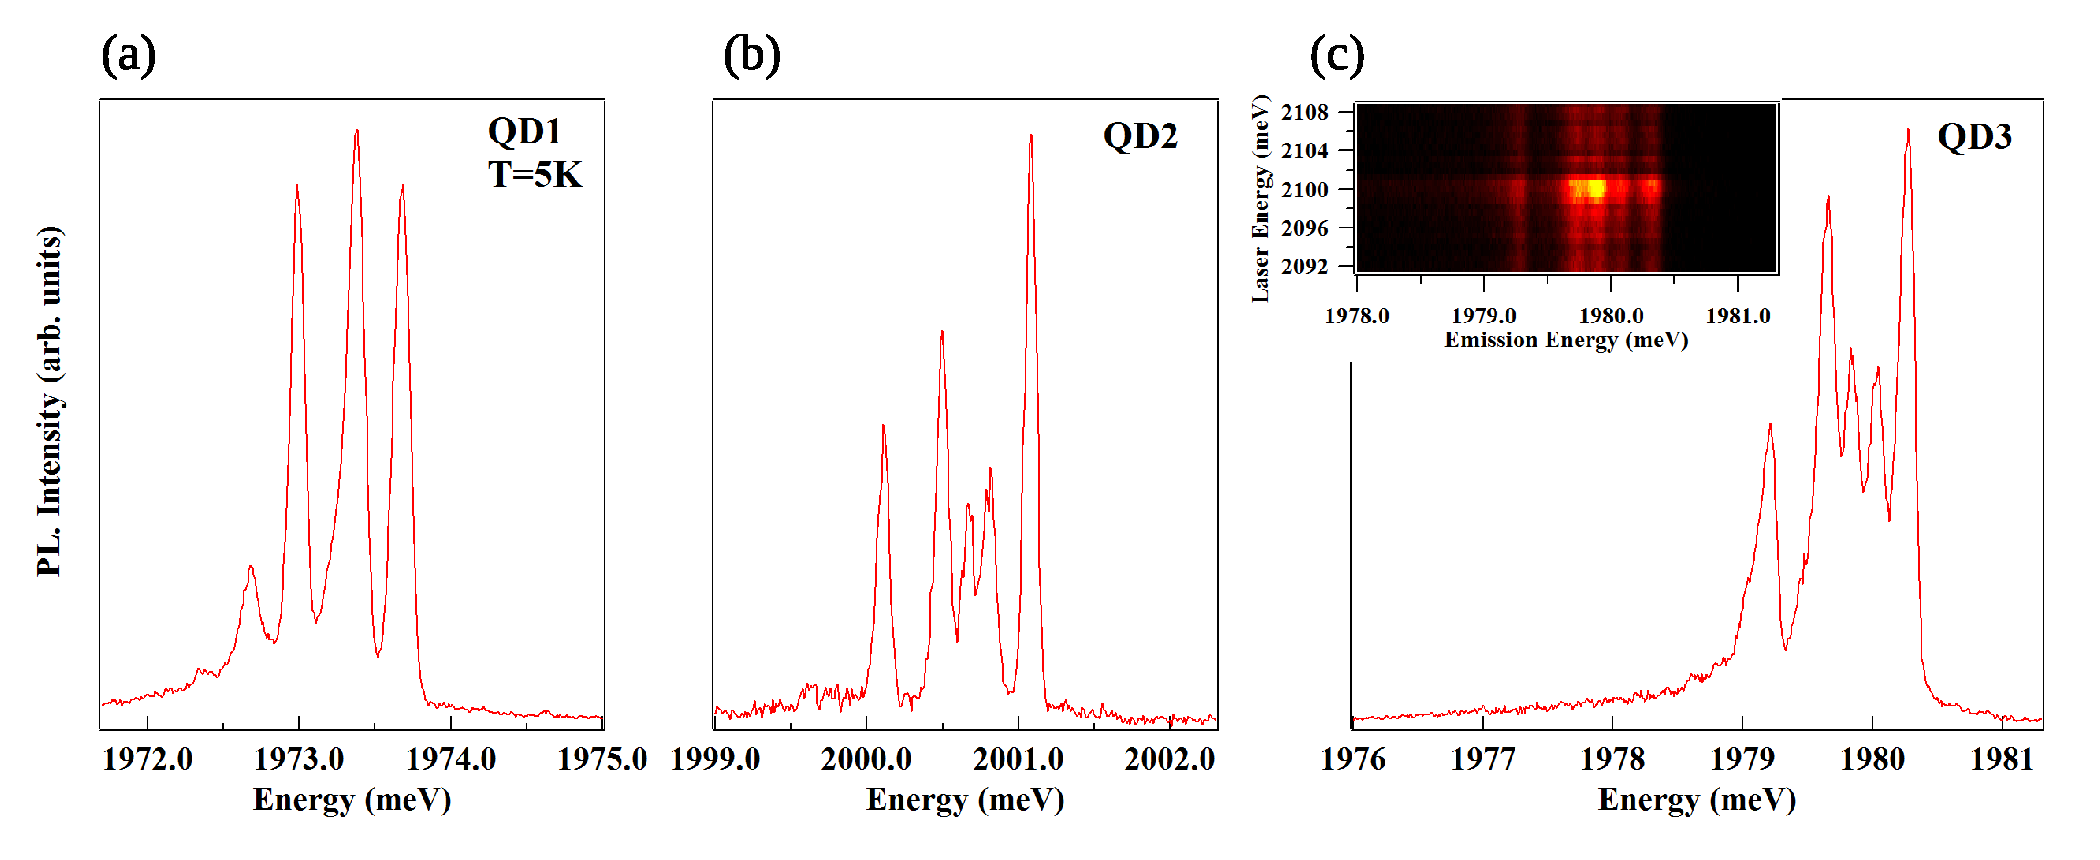
\includegraphics[width=15cm]{04-CrMagOpt/Pictures/Spectras.eps}
	\end{center}
	\caption{PL of (a) QD1, (b) QD2 and (c) QD3 X-Cr complex at low temperature (T=5K). Inset in (c) presents the PLE map of this QD, showing a sharp quasi-resonant state for an excitation at 2100 meV.}
	\label{SpectraX}
	\end{figure}

	Low temperature (T=5K) PL of the neutral exciton (X-Cr) of several QDs doped with a single Cr are reported in Fig.~\ref{SpectraX}. Characteristics three emission lines are observed, with a fourth, weaker peak on the low energy side. In some QDs, such as QD2 and QD3, the central peak was found to be split. Scanning with an energy tunable laser, we saw that all the peaks share a common quasi-resonant state, where all are at a maximum intensity, as highlighted in the inset of Fig.~\ref{SpectraX}(c). This is an indication that they originate from the same dot. Variations in the relative intensities of the peaks are observed in different dots.

	\begin{figure}[h!]
	\begin{center}
		\includegraphics[width=10cm]{04-CrMagOpt/Pictures/EnLvlantiferro.png}
	\end{center}
	\caption{Illustration of the energy levels of the ground state (Cr), the bright exciton states ($|\pm1\rangle$) coupled to the spin of a Cr (X-Cr) and dominant PL transitions ($\sigma$+, $\sigma$-). The states $S_z = \pm2$ cannot be populated through thermalization, and thus their recombination channel are not shown on this schema.}
	\label{CrEnergyStruct}
	\end{figure}

	In a II-VI semiconductor, the orbital momentum of the Cr connects the spin of the atom to its local strain environment through the modification of the crystal field and the spin-orbit coupling. For biaxial strain in the (001) plane, the ground state of a Cr spin is split by a strain induced magnetic anisotropy term ${\cal H}_{Cr,\varepsilon_\parallel}=D_0S^2_z$ (see Sec.~\ref{CrSemiCon}). It was deduced from electron paramagnetic resonance of bulk Cr-doped CdTe that $D_0$ is positive for compressive biaxial strain~\cite{EPRCr}. In a self-assembled CdTe/ZnTe QDs with large in-plane strain, the Cr spin energy levels are split from $|S_z=0\rangle$ at low energy (Fig.~\ref{CrEnergyStruct}). A value of $D_0$ in the 1 meV range can be expected for a CdTe layer strained on a ZnTe substrate, as shown in Sec.~\ref{CrSemiCon}.
	
	\begin{figure}[h!]
	\begin{center}
		\includegraphics[width=15cm]{04-CrMagOpt/Pictures/LinPol.png}
	\end{center}
	\caption{(a) Low temperature PL of QD2 recorded along two orthogonal directions. (b) Linear polarization PL intensity map of QD2. The 0$^{\circ}$ polarization angle corresponds to an emission polarized along the QD cleavage axis, either $[110]$ or $[1\bar{1}0]$. (c) Illustration of the energy levels of the ground state (Cr), the bright exciton states ($|\pm1\rangle$) coupled to the spin of a Cr (X-Cr), showing the splitting of the central peak via the bright exciton coupling, and dominant PL transitions ($\sigma$+ (blue), $\sigma-$ (red) and $\pi$ (green and black)).}
	\label{CrLinPolar}
	\end{figure}
	
	When an electron-hole pair is injected in a Cr-doped QD, the bright excitons are split by the exchange interaction between the spins of Cr and carriers. In flat self-assembled QDs, the heavy-holes and light-holes are separated in energy by the biaxial strain and the confinement. In a first approximation, the ground state in such QD is a pure heavy-hole ($J_z$=$\pm$3/2) exciton and the exchange interaction with the Cr spin S is described by the spin Hamiltonian 
	\begin{align}
		{\cal H}_{c-Cr}=I_{eCr}\mathbf{S}\cdot\bm{\upsigma}+I_{hCr}S_zJ_z
	\end{align}		
with $\bm{\upsigma}$ the electron spin and $J_z$ the hole spin operator. $I_{eCr}$ and $I_{hCr}$ are, respectively, the exchange integrals of the electron and the hole spins with the Cr spin. These exchange energies depend on the exchange constant of the Cr $3d$ electrons with the CdTe carriers and on the overlap of the Cr atom with the confined carriers. Even though the exchange interaction of the Cr spin with both electron and hole is ferromagnetic in most II-VI semiconductor~\cite{MacCdCrSD0beta,KacmanD0alphabetaIIVI,MacspdexchCr}, the hole-Cr interaction is supposed to be anti-ferromagnetic here. It does not change the PL at B = 0T. The only visible effect is on the intensity distribution in the magneto-optics experiments. This will thus be further discussed in Sec.~\ref{MagOptCr}. A typical exchange constant 4 to 5 times larger for the holes than for the electrons is also expected in CdTe~\cite{DMSCrExchInt,CdCrSExchInt}.

	\begin{figure}[h!]
	\begin{center}
		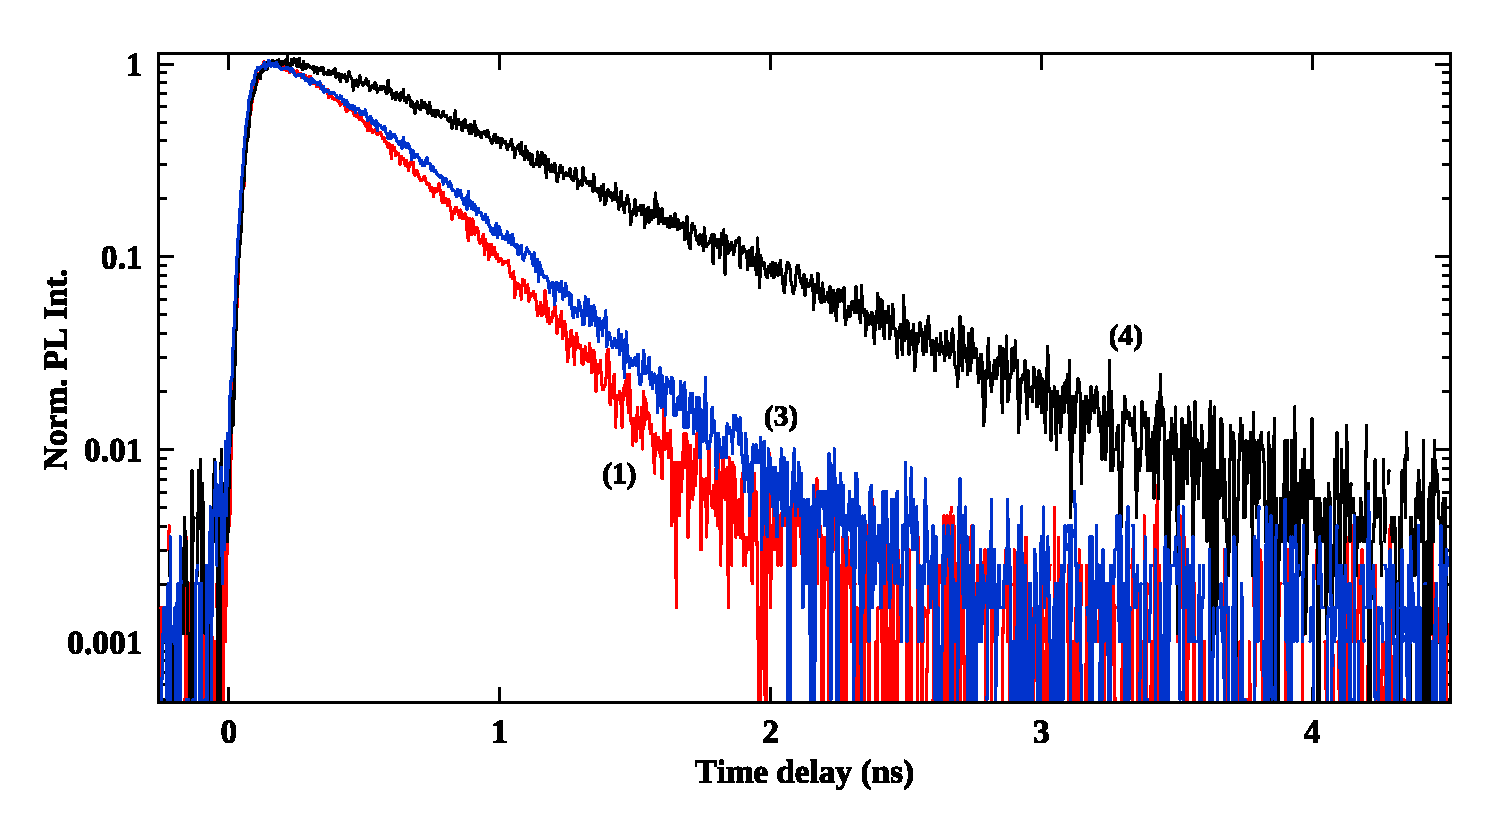
\includegraphics[width=12cm]{04-CrMagOpt/Pictures/Decay.eps}
	\end{center}
	\caption{Time resolved PL of QD2 taken on two outside peaks, attributed to $S_z = \pm1$ (noted (1) and (3) in Fig.~\ref{CrLinPolar}(a)), and the lower energy one (noted (4)).}
	\label{CrDecay}
	\end{figure}
	
	For highly strained CdTe/ZnTe QDs with a weak hole confinement, the strain induced energy splitting of the Cr spin $D_0S^2_z$ is much larger than the exchange energy with the confined carriers ($D_0\gg |I_{hCr}|>|I_{eCr}|$). The exchange interaction with the exciton acts as an effective magnetic field which further splits the Cr spins states $S_z=\pm$1 and $S_z=\pm$2. The resulting X-Cr energy levels are presented in Fig.~\ref{CrEnergyStruct}. The exciton recombination does not affect the Cr atom and its spin is conserved during the optical transitions. Consequently, the large strain induced splitting of the Cr spin is not directly observed in the optical spectra. However, at low temperature, the Cr spin thermalize on the low energy states $S_z$=0 and $S_z$=$\pm$1. This leads to a PL dominated by three contributions: a central line corresponding to $S_z=0$ and the two outer lines associated with $S_z=\pm$1 split by the exchange interaction with the carriers.
	
	Cr-doped quantum dots exhibit a linear polarization dependence, as presented in Fig.~\ref{CrLinPolar}. The central line ($S_z$=0) is split and linearly polarized along two orthogonal directions. As in non-magnetic QDs, this results from a coupling of the two bright excitons $|\pm1\rangle$ by (i) the long-range e-h exchange interaction in a QD with an in-plane shape anisotropy~\cite{SplitInvTh} and/or (ii) the short range e-h exchange interaction in the presence of valence band mixing. This anisotropic e-h exchange energy mixes the bright exciton associated with the same Cr spin state, inducing an extra splitting between them. The mixing is maximum for the central pair of bright excitons (S$_z$=0) which are initially degenerated. The outer lines are also slightly linearly polarized but the influence of the e-h exchange interaction is attenuated by the initial splitting of the $|\pm1\rangle$ excitons induced by the exchange interaction with the Cr spin$S_z=\pm1$.	

	In order to identify the lower energy peak ((4) in Fig.~\ref{CrLinPolar}(a)), we took the time resolved photoluminescence of the emission peaks, presented in Fig.~\ref{CrDecay}. One can notice that the line (4) present a decay time about twice as long as the high energy peak. Such a long decay would be coherent with the radiative recombination of a dark exciton state. Under normal circumstances, the recombination of such a state is non-radiative. However, it is possible to observe a dark exciton recombination emitting a photon in low symmetry quantum dot~\cite{DELum}. Since it is initially a forbidden transition, the recombination will be less efficient and will thus take more time~\cite{DELongLifetime}. This hypothesis will be confirmed by the magneto-optical study of the dot presented in Fig.~\ref{CrMagOptExp} and \ref{CrMagOptMod}.
	
	\begin{figure}[h!]
	\begin{center}
		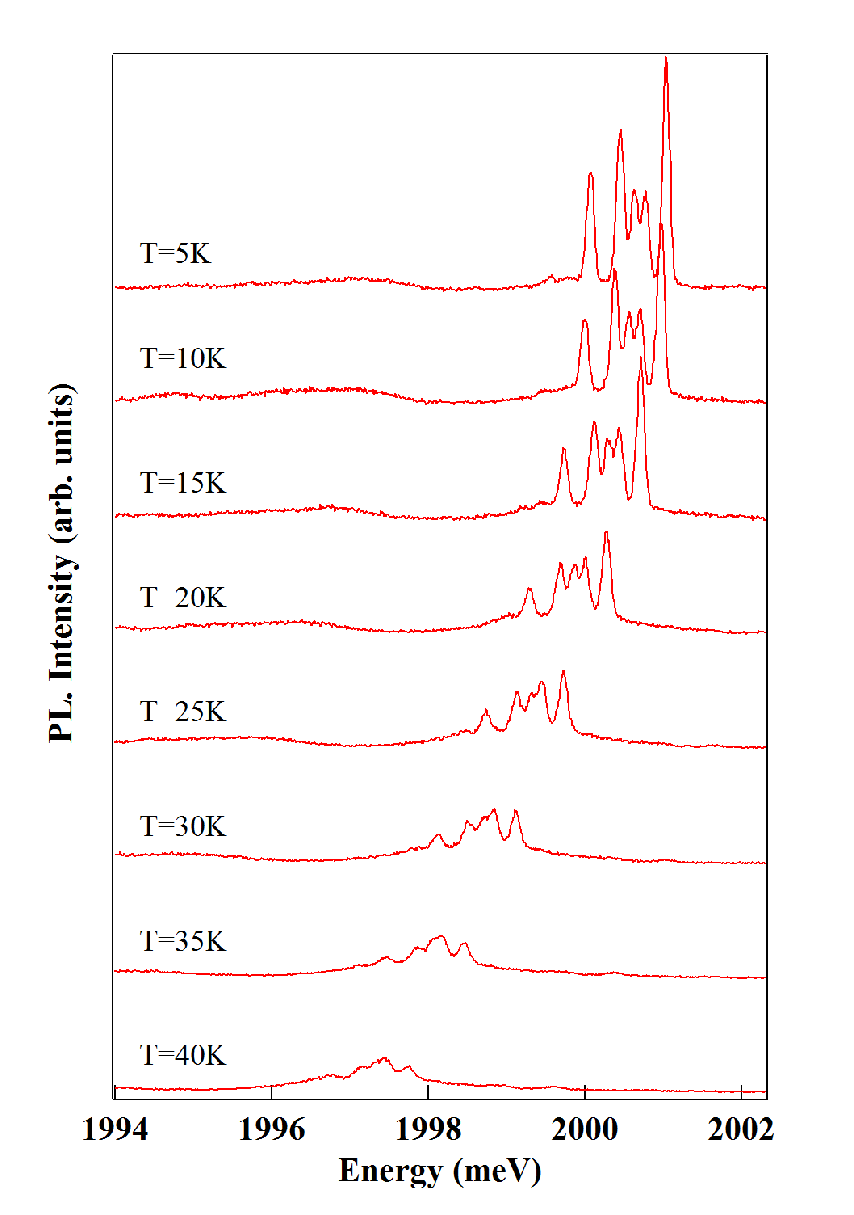
\includegraphics[width=14.9cm]{04-CrMagOpt/Pictures/Temp.eps}
	\end{center}
	\caption{Temperature evolution from T=5K to T=40K of (a) QD2 PL and (b) the PL of a QD with a good thermalisation on the low energy states (QD4). Even at 40K, $S_z = \pm2$ states do not appear.}
	\label{CrTemp}
	\end{figure}
	
	Since $S_z = \pm2$ states do not appear on the PL because they cannot be thermally populated, one could expect to see their emission at higher temperature. Fig.~\ref{CrTemp} presents the emission of two dots in function of the temperature. With the increase of the temperature, we observe a significant line broadening induced by the interaction with acoustic phonons. In order to keep a significant PL intensity and resolved PL lines, we limited our investigation to temperature below 50K. Even at this temperature, the $\pm2$ peak does not appear. Still, the figure of the emission change dramatically with the temperature. The intensity of the exterior peaks, associated with the states $\pm1$, fell quickly while the emission of the $S_z = 0$ stays intense until higher temperature. This is an unexpected picture, since the temperature should allow the higher energy states $\pm1$ to be more populated by emptying the ground state. This could be caused by a coupling to dark states, more efficient for $S_z = \pm1$ states than for $S_z = 0$ states, emptying the bright states when they are thermally populated. 
	%\newpage


		\subsection{Excited states of a Cr-doped QD}	
	
	In order to study the different excited states in a QD doped with a single Cr atom, we took the PLE of QD2 starting close to the energy of the dot's emission. Fig.~\ref{FullPLE}(a) presents the entire PLE of QD2 X-Cr complex. One can note several excited states along the scan.
	
	\begin{figure}[h!]
	\begin{center}
		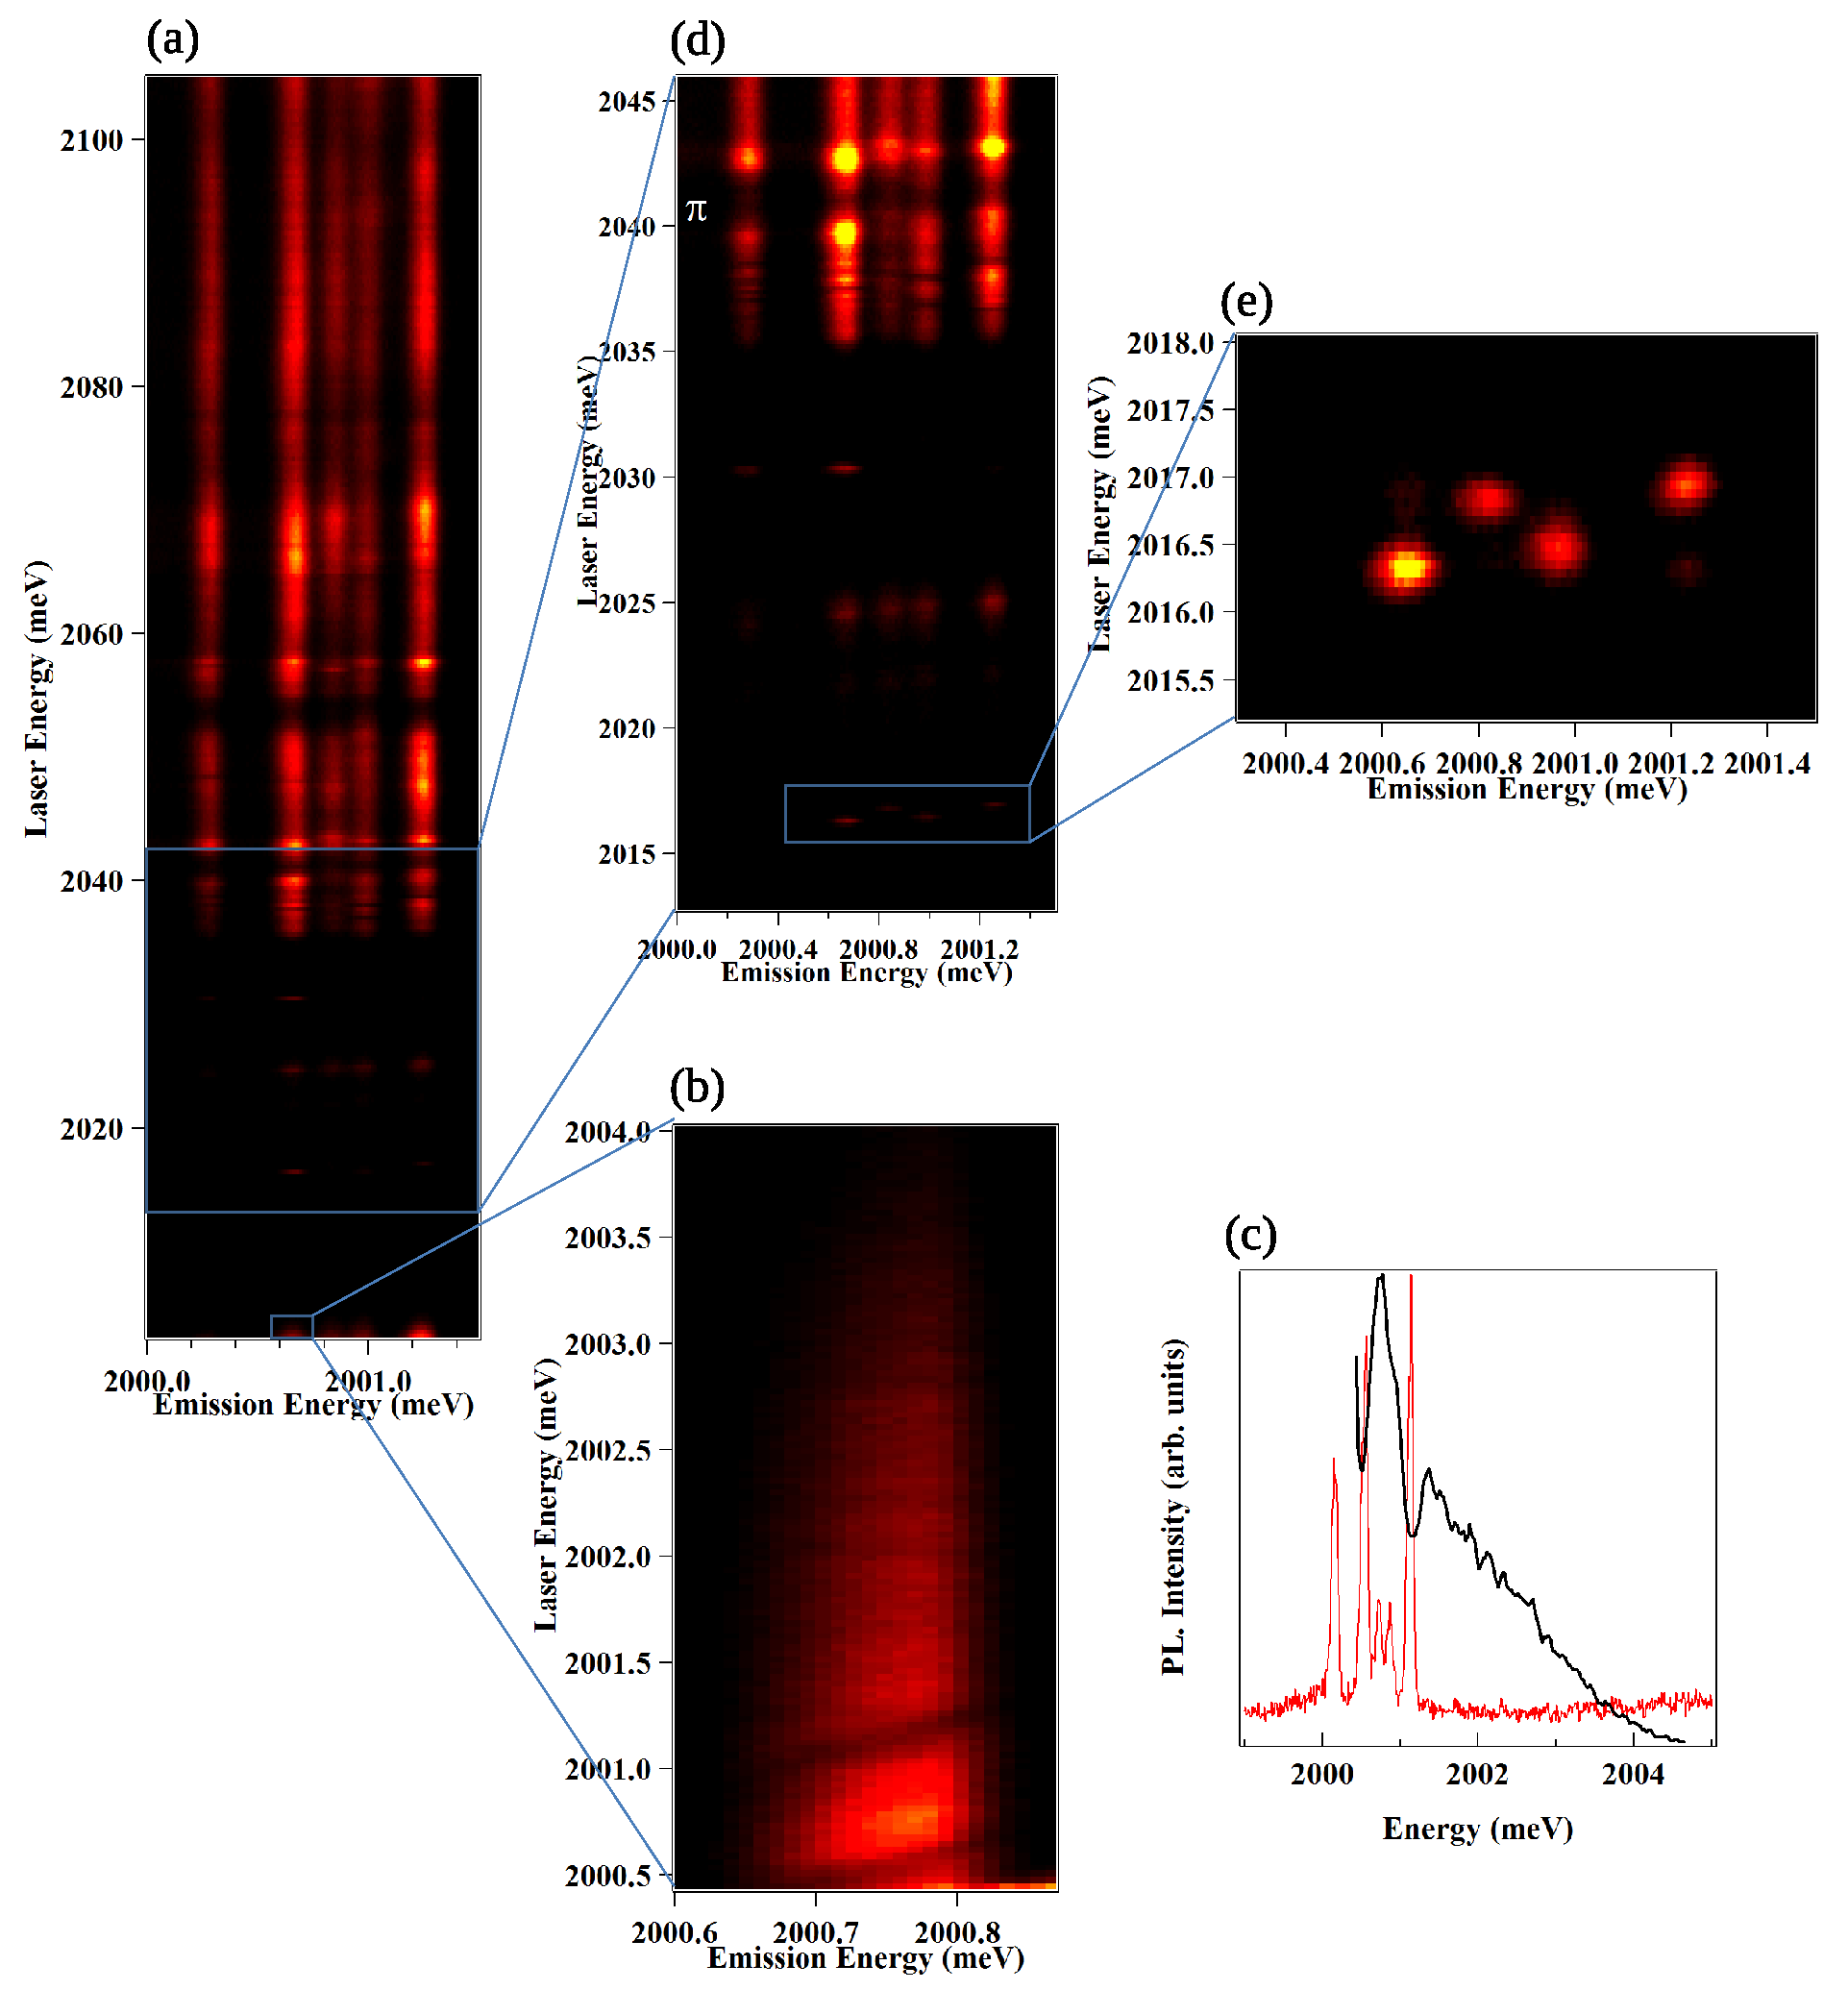
\includegraphics[width=13.8cm]{04-CrMagOpt/Pictures/FullPLEv2.eps}
	\end{center}
	\caption{(a) QD2 X-Cr PLE map in $\pi_{cross}$ polarization. Several excited states are highlighted. (b) Photoluminescence of QD2 X-Cr complex for an excitation at 2120 meV). (c) PLE scan detected on the lower energy peak, taken close to the QD emission energy, showing the phonon replica taken in $\pi$ detection. The emission integrated intensity in function of the laser energy is plotted in (d) (black curve) along with the PL spectra of QD2 taken in $\sigma_{co}$ polarization. (e) PLE map between 2046 meV and 2013 meV presenting several excited, detecting in $\pi_{cross}$ polarization. (f) Zoom in a particular excited state presented a splitting inversion, taken in $\pi_{cross}$ detection.}
	\label{FullPLE}
	\end{figure}
	
	The first remarkable feature of this scan is the luminescence over a large energy range, for an excitation between the dot emission energy and 2004 meV, zoomed in Fig.~\ref{FullPLE} (c). This corresponds to an excitation of the QD via the acoustic phonon band. 
One can notice two sharp intensity diminutions in this emission. Mapping the intensity of the phonon replica to the quantum dot spectrum (Fig.~\ref{FullPLE}(d)), it shows that these diminutions happens when the laser is in resonance with a QD emission line. The absorption then preferentially occurs in this resonantly excited state than in the acoustic phonon band.

	
	Another excited state appear around 2018.5 meV, zoomed in on Fig.~\ref{FullPLE}(f). The first feature of this peak is that, even though the studied dot contain a Cr, each of the peak here presents a slightly different resonant energy. Moreover, one can note that the order of appearance of the two central peaks seems to be reversed compared to the external ones. This phenomenon, called splitting inversion, was first observed on QDs in GaAs quantum well~\cite{FineStructSplitGaAsdots}. It has been discussed by Takagahara~\cite{SplitInvTh} and is likely due to the electron-hole exchange interaction.
	
	\begin{figure}[h!]
	\begin{center}
		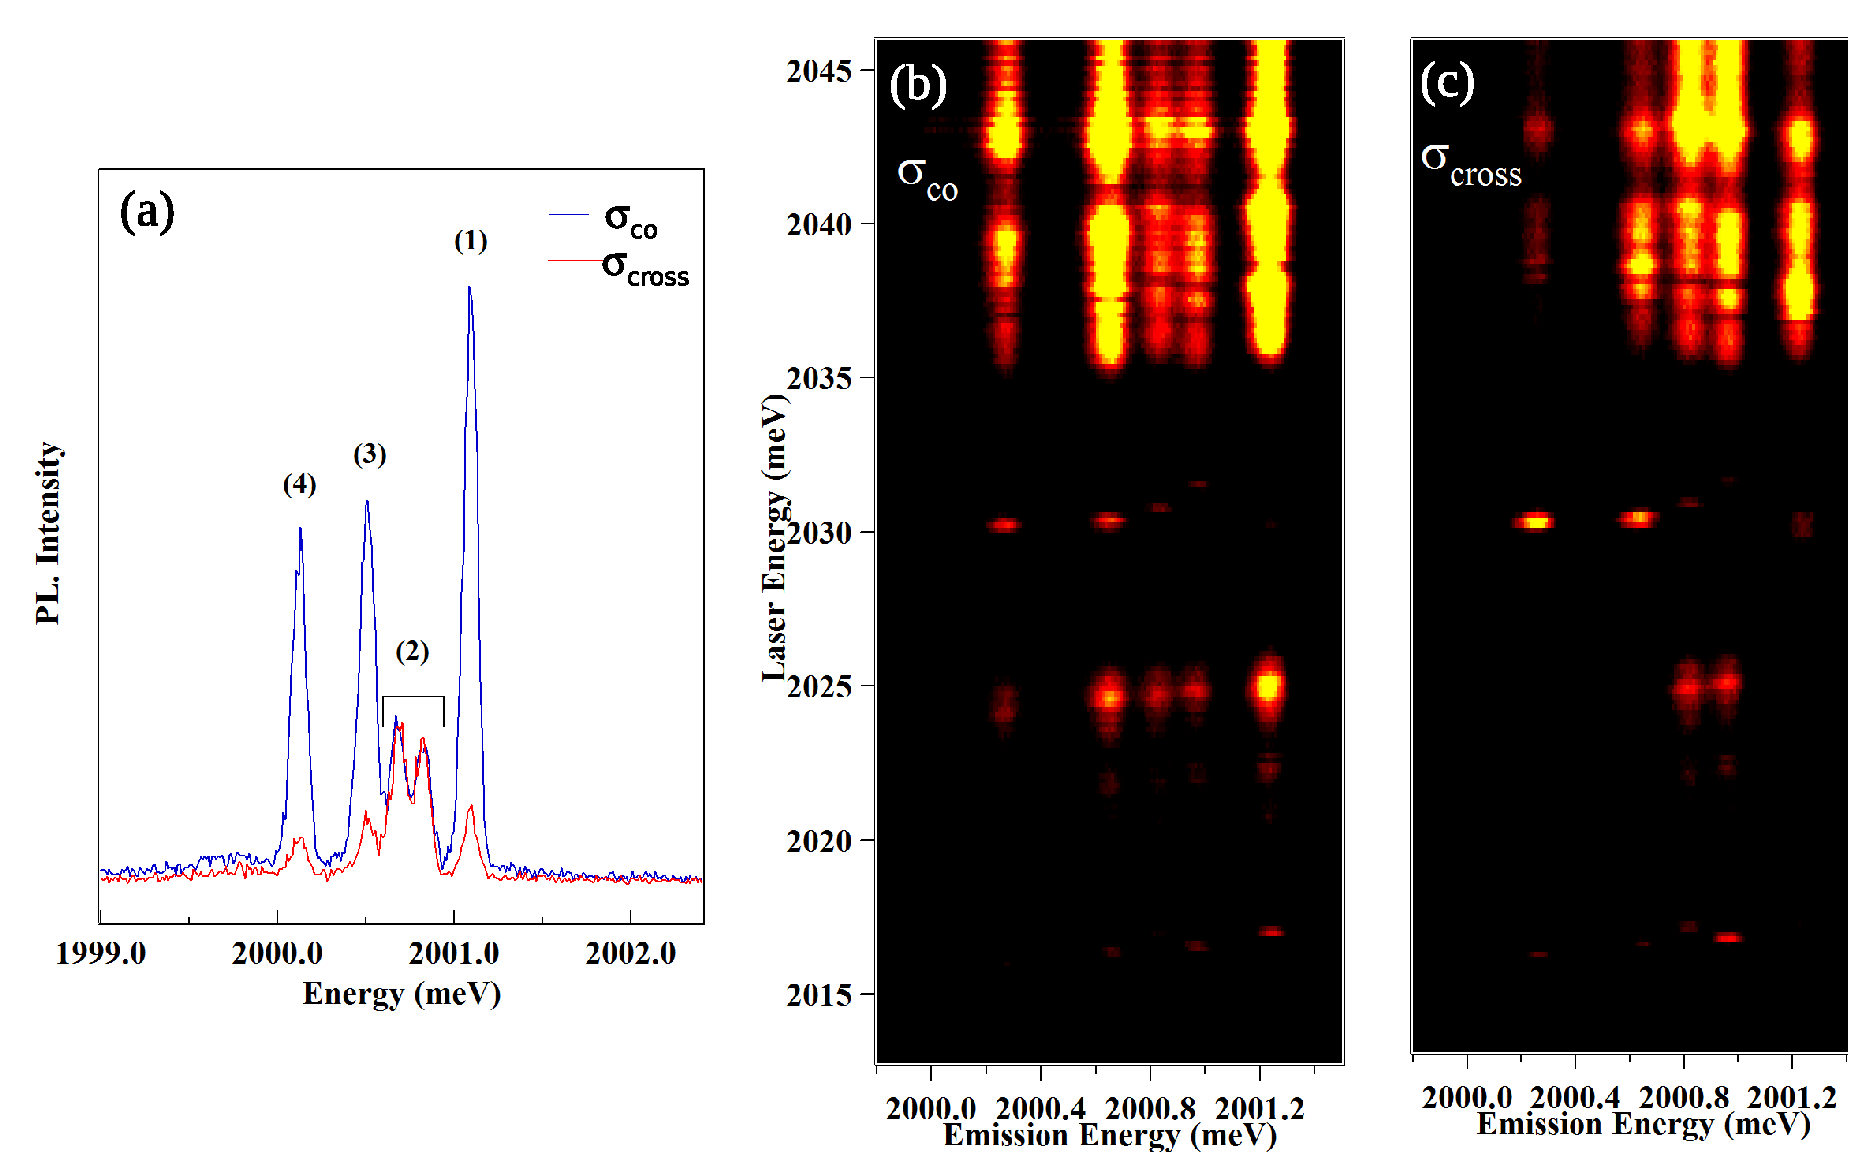
\includegraphics[width=14.9cm]{04-CrMagOpt/Pictures/PLEDotPres.eps}
	\end{center}
	\caption{(a) PL spectra of the exciton in QD2 (X-Cr) for co-circularly (blue) and cross-circularly (red) polarized excitation/detection taken on the 2120 meV quasi-resonant state. (b) - (c) PLE map between 2046 meV and 2013 meV presenting several excited states, detecting in $\sigma_{co}$ (b) and $\sigma_{cross}$ (c).}
	\label{PLEDotPres}
	\end{figure}
	
	Another excited state can be sawn at 2025 meV. It can be linked to an excitation through optical phonon. Looking at the $\sigma$ polarized emissions of this state (Fig.~\ref{PLEDotPres}(b) and (c)), we can see that the low and high energy peaks are strongly $\sigma_{co}$ polarized. It means the exciton recombining is of the same spin as the one injected by the laser, and thus shows a good spin conservation of the exciton in the QD during its lifetime. This stabilization of the exciton spin might be due to the Cr spin acting as an effective magnetic field on it. The split central peak emission is linearly polarized, as discussed in Sec.~\ref{CrPres}, and thus its emission shows no dependency in linear polarization. 
	
	Finally, another interesting excited state appear at 2030 meV. This state presents an exchange-induced splitting  different from the splitting in the quasi-resonant state, due to a difference in the carriers and Cr atom wavefunction overlap.

		\subsection{Magneto-optics of a quantum dot doped with a single Cr\label{MagOptCr}}
		
	The structure of the energy levels in Cr-doped QDs is confirmed by the evolution of the PL spectra in magnetic field (up to 11T) along the growth axis, the so called Faraday configuration~\cite{BesombesPumpMnSFD}, presented in Fig.~\ref{CrMagOptExp}. Under magnetic field, the bright exciton $X_z = \pm1$ split, leading to a $\sigma-$ branch going at low energy and a $\sigma+$ one going at high energy. This splitting of the excitonunder magnetic field can compensate the one induced by the exchange interaction with the Cr~\cite{LegerQDGeomEffect}. For QD1, this results in an anti-crossing of $|+1\rangle$ and $|-1\rangle$ excitons due to the e-h exchange interaction around B$_z$=6 T observed both in $\sigma+$ and $\sigma-$ polarizations (anti-crossing (2) and (3) in Fig.~\ref{CrMagOptExp}(a)).
		
	\begin{figure}[h!]
	\begin{center}
		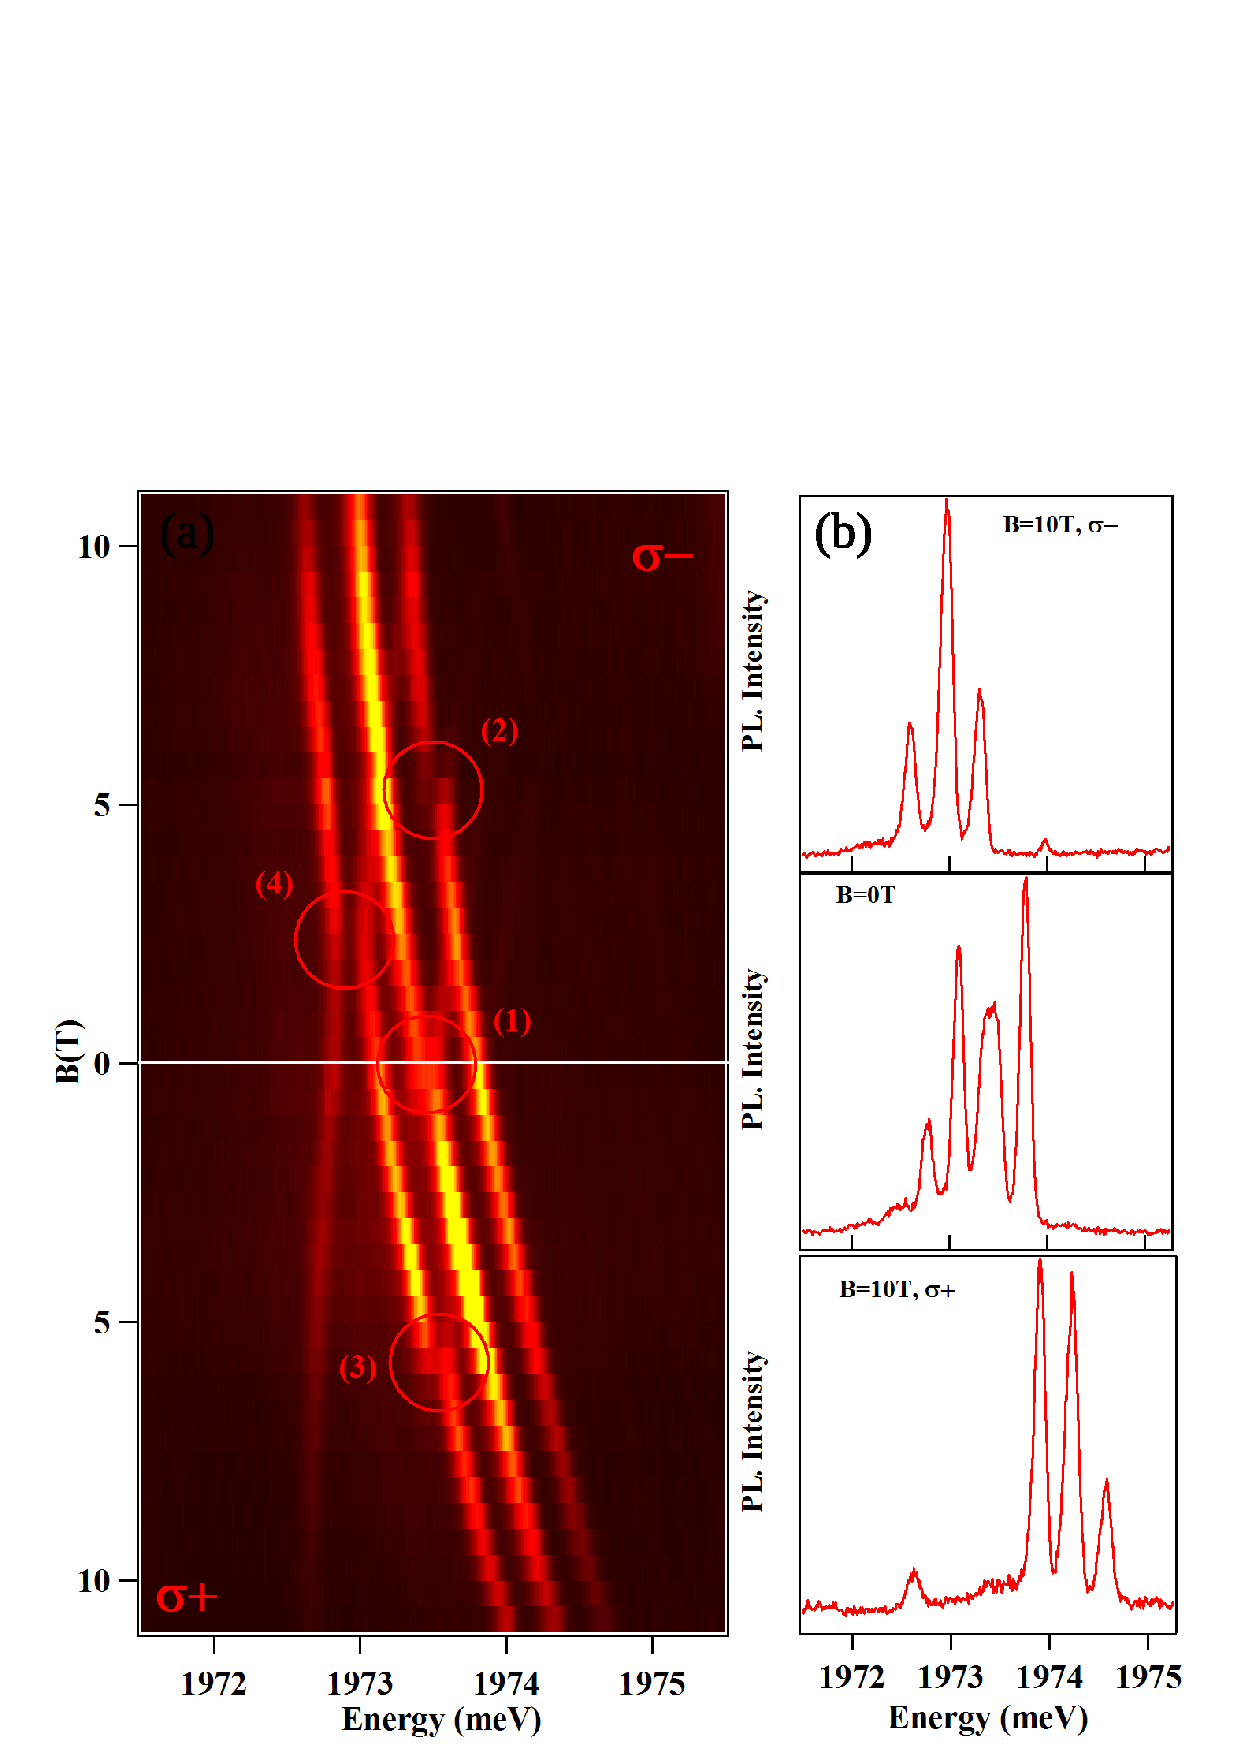
\includegraphics[width=10cm]{04-CrMagOpt/Pictures/MagOptv2.png}
	\end{center}
	\caption{(a) Circularly polarized X-Cr PL evolution under magnetic field ($B_z$) in QD1. Anti-crossings  are highlighted and numbered. (b) QD1 X-Cr PL spectra taken at 0 and $10$T for both circular polarization.}
	\label{CrMagOptExp}
	\end{figure}
		
		The low energy emission presented as a dark exciton in Fig.~\ref{CrDecay} shows an anti-crossing with the bright excitons under $B_z$ in $\sigma-$ polarization (anti-crossing (4) in Fig.~\ref{CrMagOptExp}). This anti-crossing arises from a mixing of the bright and dark excitons interacting with the same Cr spin state. Observed in $\sigma-$ polarization, it corresponds to the mixing of the exciton states $|-1\rangle$ and $|+2\rangle$ coupled to the Cr spin $S_z=+1$. This dark/bright excitons coupling $\delta_{12}$ is induced by the e-h exchange interaction in a confining potential of reduced symmetry (lower than C$_{2v}$)~\cite{DERecombTh}. In such symmetry, the dark exciton acquire an in-plane dipole moment which leads to possible optical recombination at zero magnetic field~\cite{DELum} as observed in these QDs. The oscillator strength of this "dark exciton" increases as the initial splitting between $|-1\rangle$ and $|+2\rangle$ excitons is reduced by the magnetic field.
		
	\begin{figure}[h!]
	\begin{center}
		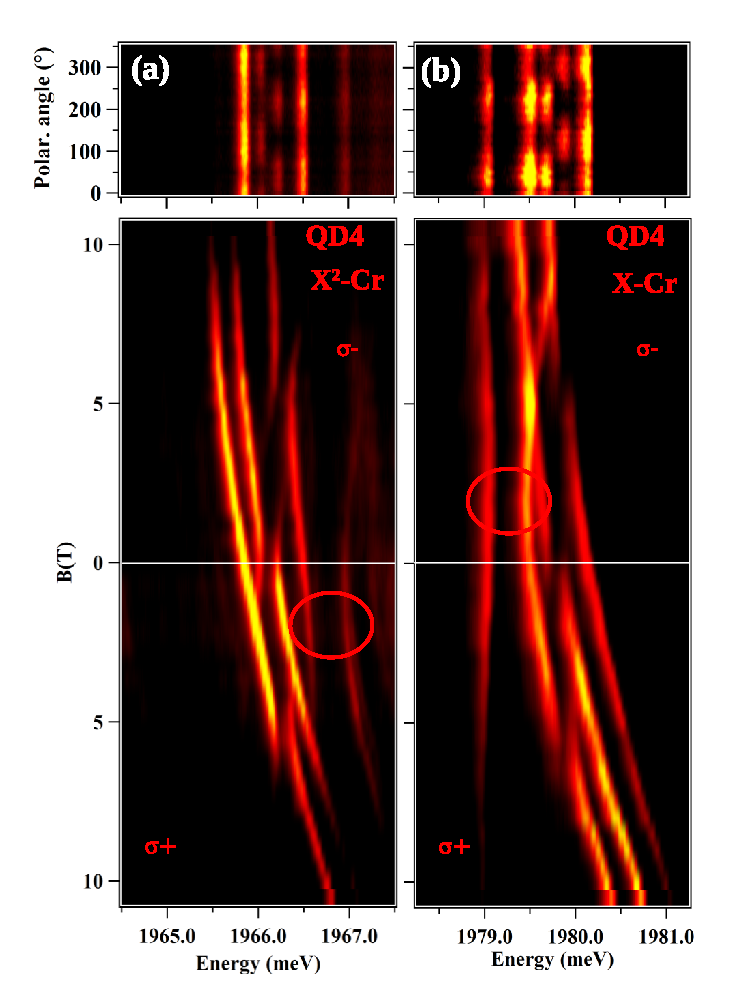
\includegraphics[width=10cm]{04-CrMagOpt/Pictures/MagOptLowSym.eps}
	\end{center}
	\caption{Linear polarization intensity map (top panel) and intensity map of the longitudinal magnetic field dependence of the emission (bottom panel) of (a) X$^2$-Cr and (b) X-Cr in QD3.}
	\label{CrMagOptLowSym}
	\end{figure}
		
		To illustrate the influence of the QD symmetry on the magneto-optical properties of X-Cr, we show in Fig.~\ref{CrMagOptLowSym}(b) the emission of a QD with a different strain or shape anisotropy (QD3). For QD1, the splitting of the central peak is not clear in the PL at 0T (Fig.~\ref{SpectraX}(a)), while two linearly polarized peaks appears clearly in QD3 spectra (Fig.~\ref{SpectraX}(c)).
		
		Investigating both the biexciton and the exciton in the same Cr-doped QD, we can also analyze the impact of the carrier-Cr interaction on the fine structure of the Cr spin. The magnetic field dependency of X$^2$-Cr emission in QD3 is presented along with the X-Cr emission as a contour plot in Fig.~\ref{CrMagOptLowSym}(a) and (b) respectively. The PL under magnetic field of X-Cr and X$^2$-Cr presents a mirror symmetry. In particular, the dark/bright exciton mixing observed around $B_z=2.5$ T on the low energy side of the PL in $\sigma-$ polarization for X-Cr is observed on the high energy side in $\sigma+$ polarization for X$^2$-Cr (circles in Fig.~\ref{CrMagOptLowSym}(a) and (b)).
		
	\begin{figure}[h!]
	\begin{center}
		\includegraphics[width=10cm]{04-CrMagOpt/Pictures/Antiferro-Cr.eps}
	\end{center}
	\caption{(a) Evolution in magnetic field of QD4 X-Cr circularly polarized PL. (b) QD3 X-Cr PL at $B_z = 0$ T and $B_z = 7$ T in both polarization. }
	\label{CrAntiferro}
	\end{figure}
		
		If one consider the ground state of X$^2$ as a spin-singlet (total spin 0), it cannot be split by the magnetic field or the spin interaction part of the carriers-Cr hamiltonian. The creation of two excitons in the QD cancels the exchange interaction with the Cr atom. Thus, the PL of  X$^2$-Cr is controlled by the final state of the optical transitions, i.e. the eigenstates of X-Cr, resulting in the observed mirror symmetry in the PL spectra.
		
	\begin{figure}[h!]
	\begin{center}
		\includegraphics[width=10cm]{04-CrMagOpt/Pictures/Antiferro-Mn.eps}
	\end{center}
	\caption{(a) Evolution in magnetic field of the PL of a single Manganese atom coupled to an exciton in a II-VI QD. (b) PL spectra of the X-Mn system taken at $B_z = 0$ T and $B_z = 11$ T in both circular polarization. These experimental results are taken from Yoan L\'eger PhD thesis~\cite{YoanTh}.}
	\label{MnAntiferro}
	\end{figure}
		
	The evolution under magnetic field of the relative intensity of each of the QD peak gives information on the sign of the interaction between the Cr and the hole spin. As shown in Fig.~\ref{CrEnergyStruct}, given a polarization, each peak can be linked to a Cr spin state. As discussed earlier, applying a magnetic field lifts the degeneracy between the exciton states and allows to efficiently select the polarization of the emission. The evolution of the peaks relative intensities under magnetic thus gives information on the hole-Cr exchange interaction sign.
	
	QD4, presented in Fig.~\ref{CrAntiferro}, presents a clear evolution of the intensity under magnetic field and will be used for this study. The central peak intensity stays the stronger of the three peaks, whatever the direction of the magnetic field. This is expected, since the $S_z = 0$ state is not affected by the Zeeman effect. It remains the lower spin state for the Cr atom, and therefore concentrate most of the population. In the $\sigma-$ branch, the high energy peak get brighter while the low energy one disappear for $B_z \geq 8$T in QD4. The situation is opposite in the $\sigma+$ branch, where the intensity concentrate on the lower energy peak.
	
	This evolution is similar as the one observed in II-VI QDs doped by a single Mn atom, presented in Fig.~\ref{MnAntiferro}. It was shown in Yoan L\'eger PhD thesis~\cite{YoanTh} that the $S_z = -\frac{5}{2}$ state of the Mn atom was stabilized under magnetic field. From the evolution of the peaks relative intensity and the polarization of the different Mn states, it was then possible to deduce that the interaction between Mn and hole was anti-ferromagnetic.
	
	The evolution of the peaks relative intensity for the Cr looks like the one for the Mn. Under magnetic field, the $S_z = -1$ is stabilized, becoming the lower energy state of the doublet $S_z = \pm1$. For a high enough magnetic field, we can only consider the recombination toward $S_z = -1$. The high energy peak corresponds then to the $|S_z = -1, X_z = -1\rangle \rightarrow |S_z = -1\rangle$ on, emitting a $\sigma-$ polarized photon. The low energy one is associate with the $|S_z = -1, X_z = +1\rangle \rightarrow |S_z = -1\rangle$ transition, emitting a $\sigma+$ polarized photon. This is coherent with an anti-ferromagnetic coupling between the Cr and hole, contradicting the assumption made in Sec.~\ref{CrCdTe} and confirming the energy structure presented in Fig.~\ref{CrEnergyStruct}.
		
	\section{Modelization of a Cr-doped QD\label{QDParam}}
	
	We calculated the magneto-optic behaviour of Cr-doped QDs by diagonalizing the complete Hamiltonian of the e-h-Cr in self-assembled dots. We use for this purpose a spin effective hamiltonian that can be separated as follows:
	
	\begin{align}
\label{X-Cr} {\cal H}_{X-Cr}={\cal H}_{Cr,\varepsilon}+{\cal H}_{cCr}+{\cal H}_{mag}+{\cal H}_{eh}+{\cal H}_{band}+{\cal H}_{scat}
	\end{align}
where:

${\cal H}_{Cr,\varepsilon}$ describes the fine structure of the Cr atom and its dependency on local strain, as presented in Eq.~\ref{Cralone}. It is mainly drived by $D_0$, the magnetic anisotropy. E, the in-plane strain anisotropy, also appears in this Hamiltonian, but have to be kept small in order to model the found dots (see Fig.~\ref{CrHighE} for the emission of a dot with a higher E).

\begin{figure}[h!]
	\begin{center}
		\includegraphics[width=14.9cm]{04-CrMagOpt/Pictures/SimuAntiferro.png}
	\end{center}
	\caption{(a) Top: Calculated linear polarization PL intensity map of X-Cr at zero field. The 0$^{\circ}$ polarization angle correspond to an emission polarized along the $[100]$ axis. Bottom: Calculated X-Cr circularly polarized magnetic field dependency. Details of the model and parameters are listed in Tab.~\ref{CrModelParam}. Corresponding anti-crossing are highlighted in same fashion as on Fig.~\ref{CrMagOptExp} and \ref{CrAntiferro}. On the left, spectra calculated for $B_z = 0$ T and $B_z = 11$ T in both circular polarization are shown. (b) Schema of the magnetic field dependency of the energy levels of the low energy Cr spin states $S_z$=0 and $S_z$=$\pm$1, and corresponding bright ($+1$ blue, $-1$ red) and dark ($|\pm2\rangle$ green) X-Cr energy levels.}
	\label{CrMagOptMod}
	\end{figure}

${\cal H}_{cCr}$ describes the coupling of the electron and hole with the Cr spin, depending on $I_{eCr}$, the exchange integral of the electron-Cr spins, and $I_{hCr}$, the exchange integral of the hole-Cr spins, as described in Eq.~\ref{HCrDMS}.

${\cal H}_{mag}$ describes the effect of an exterior magnetic field, coupled to both the Cr and carrier spins by the Zeeman terms, depending on the $g$-factor of each of them and the Bohr magneton $\mu_B$, and including the diamagnetic shift of the electron-hole via the term $\gamma$.
\begin{align}
	{\cal H}_{mag} = g_{Cr}\mu_B\overrightarrow{B}.\overrightarrow{S}+g_{e}\mu_B\overrightarrow{B}.\overrightarrow{\sigma}+g_{h}\mu_B\overrightarrow{B}.\overrightarrow{J}+\gamma B^2
\end{align}

${\cal H}_{eh}$ describes the short range and long range electron-hole interaction, through the bright and dark exciton splitting $\delta_0$, the bright exciton coupling $\delta_1$, the dark exciton coupling $\delta_2$ and the bright and dark exciton coupling $\delta_{11}$ and $\delta_{12}$. All of these term are described in Eq~\ref{HehCs}.

${\cal H}_{band}$ is the band Hamiltonian. It is written ${\cal H}_{band} = E_g + {\cal H}_{VBM}$, with $E_g$ the CdTe gap energy and ${\cal H}_{VBM}$ is described in Eq.~\ref{HVBM}.

${\cal H}_{scat}$ describes the perturbation of the wave function of the exciton in the initial state of the optical transition by the hole-Cr exchange interaction, controlled by the parameter $\eta$. It was found to be essential to explain the dynamic of X$^+$-Mn and is introduced here for generality purpose. This perturbation depends on the value of the exchange energy between the Cr spin $S_z$  and the hole spin $J_z$ and can be represented, using second order perturbation theory, by an effective spin Hamiltonian \cite{CarInSpinSplit,BiexFinStruct,DynhMn}
\begin{align}
{\cal H}_{scat}=-\eta S_z^2
\end{align}
\noindent with $\eta>0$.

	We considered the general case of QDs with a symmetry lower than C$_{2v}$ (truncated ellipsoidal lens for instance~\cite{DERecombTh}), and took into account the influence of this reduced symmetry on the valence band and on the e-h exchange interaction. The population of the X-Cr spin states split by the large magnetic anisotropy and the carriers-Cr exchange interaction is described by a spin effective temperature $T_{eff}$, applied on the X-Cr levels and the initial state of the hamiltonian. The results of the model obtained with $T_{eff}=$20K, $D_0=2.2$ meV and an electron-Cr (hole-Cr) exchange interaction $I_{eCr}=-50$ $\mu$eV ($I_{hCr}=250$ $\mu$eV) are reported in Fig.~\ref{CrMagOptMod} (parameters not specific to Cr-doped QDs are listed in Tab.~\ref{CrModelParam}). Such parameters do not aim to fit the data and are only reasonable order of magnitude to qualitatively reproduce the experimental results of the PL of X-Cr at zero field and its evolution in magnetic field. The splitting of the central line at zero field (anti-crossing (1)) and the anti-crossings under magnetic field (anti-crossings (2) and (3) around $B_z$=6T for the Cr spin states  $S_z = |+1\rangle$ and anti-crossings (4) with the dark exciton around $B_z$=2T) are well reproduced by the model.
	
	This model also predicts an anti-crossing around $B_z = 5$ T, noted (5), caused by an electron-Cr flip flop, which is not sawn on the experiments. Its position is controlled by $D_0$ and its intensity by $I_{eCr}$. However, for this anti-crossing to appear for $B_z > 11$T, a $D_0 > 3$ meV is needed, causing the $S_z = \pm1$ levels to be at high energy and thus giving a stronger emission intensity to the $S_z = 0$ state than the one sawn experimentally. Therefore, a low value of $I_{eCr}$ was chosen instead. Finally, the remaining tail of an anti-crossing, labelled (6), also appears at high magnetic field in the $\sigma-$ polarization, as saw in Fig.~\ref{CrAntiferro}, due to the coupling a bright and a dark exciton coupled to the Cr state $S_z = 0$.

	


\begin{table}[t] \centering
	\caption{Values of the parameters used in the model of Cr-doped CdTe/ZnTe quantum dot presented in Fig.~\ref{CrMagOptMod}. The value of the parameters not listed in the table is 0. The chosen values are typical for CdTe/ZnTe quantum dots and can be compared with parameters extracted from Mn-doped quantum dots \cite{DynhMn,DELum}. These values are reasonable to reproduce the emission of the QDs presented in this thesis.}
	\begin{tabular}{p{0.9cm}p{0.9cm}p{0.9cm}p{0.9cm}p{0.9cm}p{0.9cm}p{0.9cm}p{0.9cm}}
\hline\hline
I$_{eCr}$ & I$_{hCr}$ & $\delta_0$ & $\delta_1$ & $\delta_{12}$ & $\delta_{11}$ & $\frac{|s|}{\Delta_{lh}}$ & $\frac{|r|}{\Delta_{lh}}$ \\
$\mu eV$ & $\mu eV$ & $meV$ & $\mu eV$ & $\mu eV$ & $\mu eV$ &  & \\
\hline
-50 & 250 & -1 & 250 & 150 & 50 & 0.05 & 0.05 \\
\hline\hline 
	\end{tabular}
	\begin{tabular}{p{0.9cm}p{0.9cm}p{0.9cm}p{0.9cm}p{0.9cm}p{1.3cm}p{0.9cm}p{0.9cm}}
arg(r) & $D_0$ & $g_{Cr}$ & $g_{e}$ & $g_{h}$ & $\gamma$ & $\eta$ & $T_{eff}$ \\
 & $meV$ & &  &  & $\mu eV/T^2$ & $\mu eV$ & K \\
\hline
$-\dfrac{\pi}{2}$ & 2.2 & 2 & -1 & 0.4 & 1.5 & 25 & 20 \\
\hline\hline
	\end{tabular}
	\label{CrModelParam}
	\end{table}
	
	The magnetic anisotropy $D_0$ cannot be precisely extracted from the PL spectra. However, for $D_0 <  2$ meV, an anti-crossing due to a VBM induced hole-Cr flip-flop between the $|-1, +2\rangle$ and the $|0, -1\rangle$ would appear below B$_z$=11T on the central line in $\sigma-$ polarization. Moreover, as discussed earlier, a $D_0 > 3$ meV would produce a lower PL intensity for the states $S_z = \pm1$. These consideration sets a $D_0$ in the range of 2 to 3 meV. However, even in this range, the intensity distribution of the PL cannot be perfectly reproduced: while the intensity ratio of the peaks is quite well predicted for high value of the magnetic field, the $S_z = 0$ state still present a stronger emission at $B_z = 0$T than the one observed in the experiments. This difference in intensity may be due to out of equilibrium phonons in the sample that help populating the $S_z = \pm1$ states.

	Our model reproduce qualitatively with enough satisfaction the data found experimentally and thus can be used to see the evolution of the emission varying different parameter. Especially, an interesting point is the influence of the anisotropy of strains on the emission. The results of the calculations are presented on Fig.~\ref{CrHighE}.
	
	\begin{figure}[h!]
	\begin{center}
		\includegraphics[width=13cm]{04-CrMagOpt/Pictures/HighE.eps}
	\end{center}
	\caption{Calculated X-Cr linear polarization intensity map at B = 0T (top) and circularly polarized magnetic dependency (bottom) for dot with an anisotropy of strains (a) $E = 25$ $\mu$eV and (b) $E = 100$ $\mu$eV.}
	\label{CrHighE}
	\end{figure}
	
	The linear polarization dependency of the PL shows a splitting of all the three peaks at 0T, strengthening for a higher anisotropy of strain. 
In-plane strain anisotropy lead to Valence Band Mixing via the Bir-Pikus hamiltonian, as presented in Sec.~\ref{VBM}. Bright excitons mixed this way presents a linearly polarized emission. However, bright excitons levels are split when coupled to Cr spin states $S_z = \pm1$, acting as an effective magnetic field. A small anisotropy of strain cannot couple those, and thus they do not present linear polarization. Increasing the value of the anisotropy make it possible for these levels to be coupled, giving their emission a linear polarization dependency.

	The anisotropy of strain also affects the anti-crossing appearing of the magnetic field dependency. The anti-crossings (1) through (6) remain but we decided not to highlight them for the sake of clarity. Three new anti-crossings appear when increasing the value of $E$. Anti-crossings (8) and (9), on the outside peaks at B = 0T, are caused $E$ induced VBM discussed in the previous paragraph. Anti-crossing (7), on the high energy peak at roughly the same magnetic field value and direction as anti-crossing (4), appears when $|S_z = +1, X_z = -1\rangle$ and $|S_z = -1, X_z = -1\rangle$ are brought together by the magnetic field. They are coupled by the $E$ term, coupling two levels separated by two units of spin, via an electron-hole flip flop.

	For a higher value of $E$, the anti-crossings are stronger. They occur on a larger range of energy, and  with a wider split for the anti-crossing (8) and (9). This leads to a superposition of the different anti-crossing, giving a complex magnetic dependency and the apparent reduction of the splitting at B = 0T.
	
	Most of the dot we found presented a small anisotropy. The reason might be a selection bias. The splitting at zero magnetic field leads to a spectra with six different peaks. Moreover, we saw on Fig.~\ref{CrHighE} (b) that the splitting at B = 0T can be reduced due to the width of the anti-crossings. The resolution of our monochromator might then not be precise enough to resolve the peaks, and only shows a broad emission. Such a dot would then not be selected for further studies, leading to a selection bias toward low anisotropy dots.
	
	\section{Charge fluctuation of a Cr ion  in the vicinity  of the QDs}
	
	Some dots were found presenting a linear polarization dependency all their peaks, for both X-Cr and X$^2$-Cr. One of them, QD5, is presented on Fig.~\ref{CrSixPeaksMagOpt}. Such a dependency is expected in dots with a strong in-plane anisotropy, as shown in Sec.~\ref{QDParam}. While a thin and well resolve X$^+$-Cr is observed on all these dots, X-Cr is often not resolved, appearing as a broad emission. Such a result was also expected for dots with strong in-plan anisotropy.
	
	\begin{figure}[h!]
	\begin{center}
		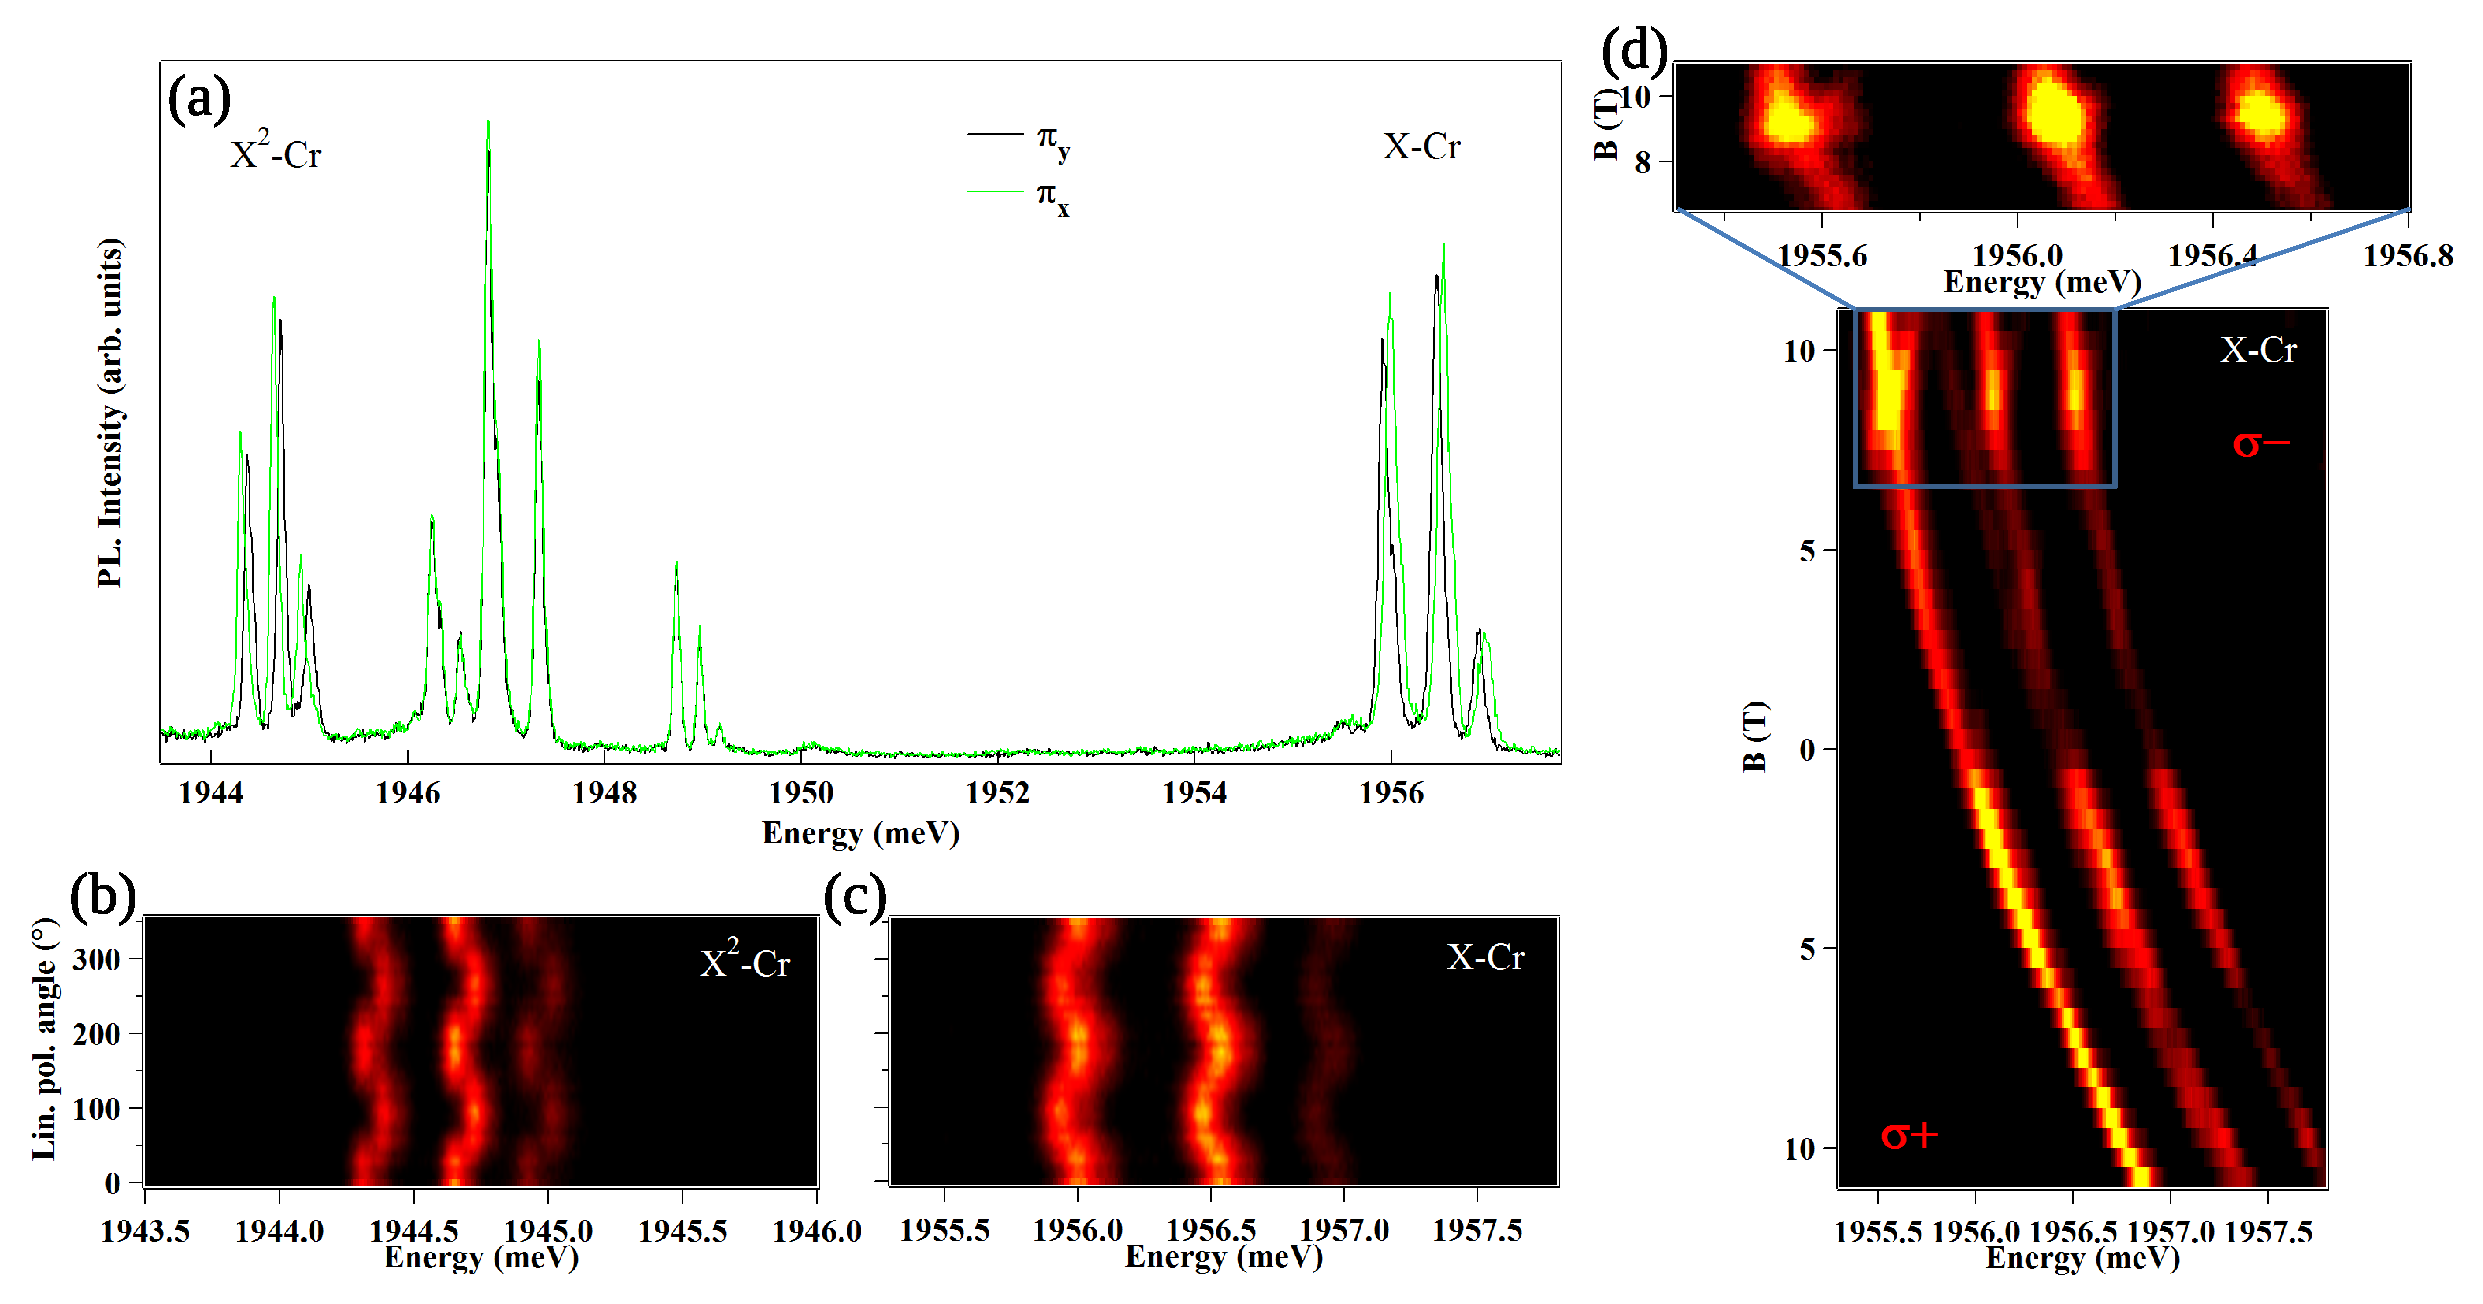
\includegraphics[width=14.9cm]{04-CrMagOpt/Pictures/6peaks.eps}
	\end{center}
	\caption{(a) QD5 linearly polarized PL intensity at zero magnetic field. (b) and (c) Respectively QD5 X$^2$-Cr and X-Cr linear polarization PL dependence at zero magnetic field. (c) X-Cr magnetic field PL dependence of QD5. Zoom in presents anti-crossing appearing at B=9T.}
	\label{CrSixPeaksMagOpt}
	\end{figure}
	
	However, studying the dot under magnetic field show no appearance of the expected anti-crossing for a QD with a high in-plane anisotropy. The dots present a single anti-crossing on all their peaks for B = 9T in $\sigma-$ polarization. It is due to the mixing between bright and dark exciton. Such an evolution under magnetic tend to characterise three non-magnetic QDs emitting at close energy. However, all the peaks were found to have the maximum intensity for the same position on the sample, and they share excited states on the PLE. It is highly improbable to find three dots close to each other, emitting almost at the same energy and sharing excited states at several position on the sample. 

	\begin{figure}[h!]
	\begin{center}
		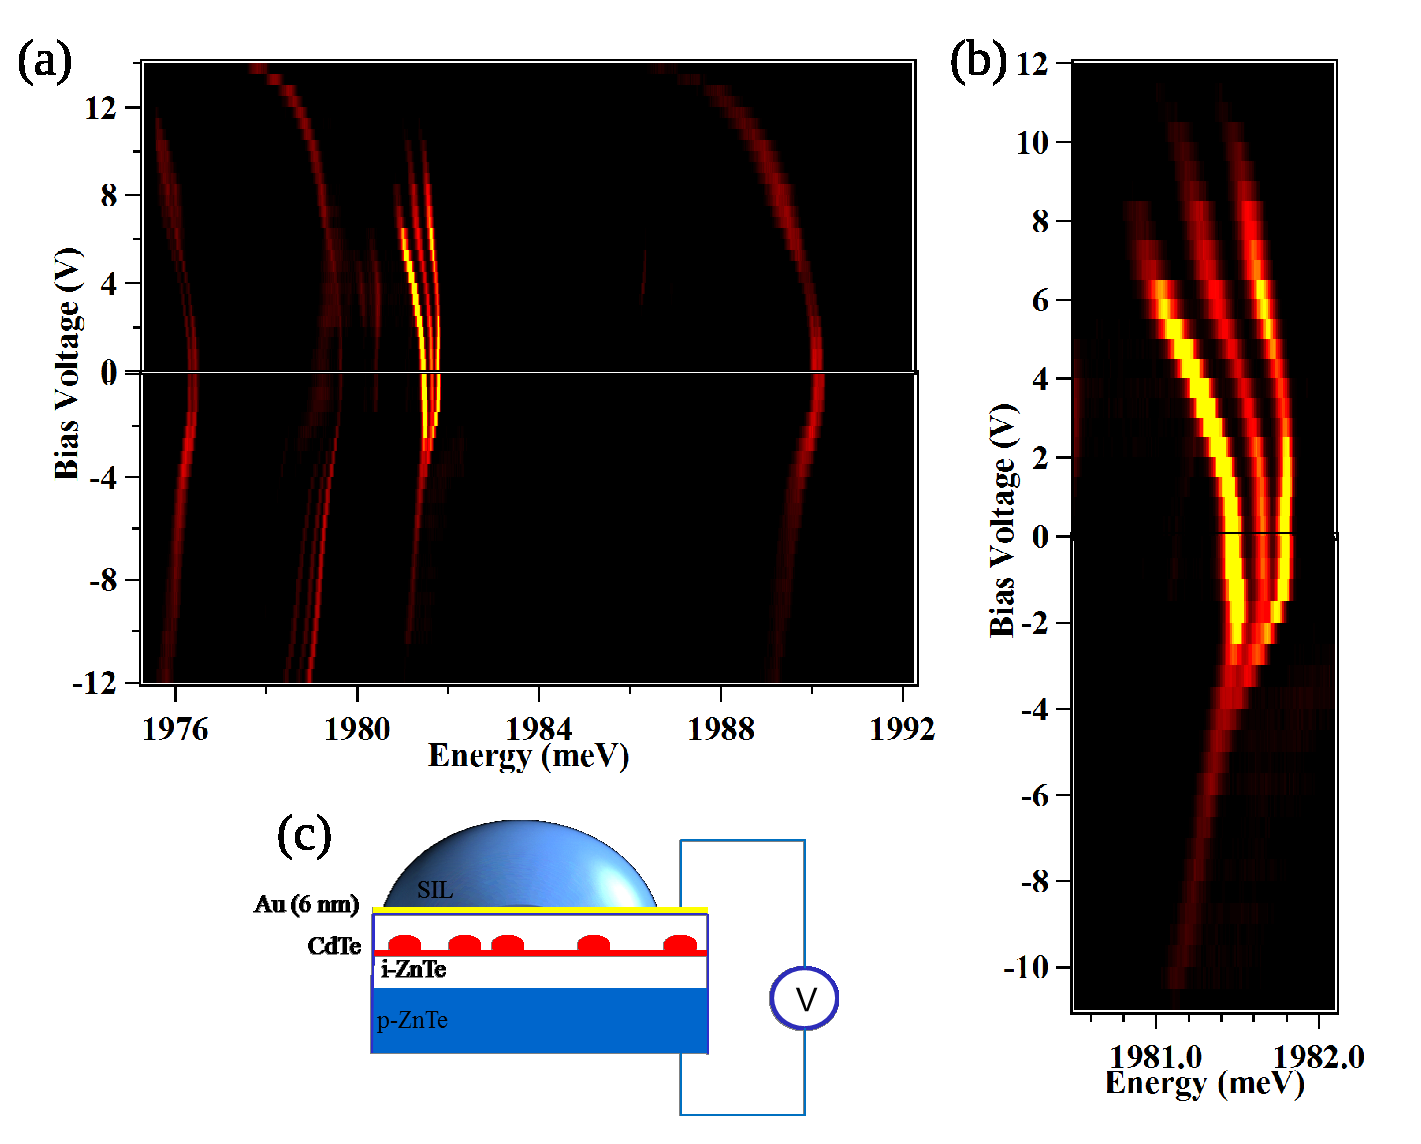
\includegraphics[width=12cm]{04-CrMagOpt/Pictures/EfieldX-Xc.eps}
	\end{center}
	\caption{(a) QD7 whole PL evolution under application of a bias voltage. (b) Zoom on X$^c$-Cr circular polarization PL intensity evolution under electric field. A strong stark shift is observed, as well as variation in the splitting. (c) Schema of a sample with a Schottky gate used to apply the bias voltage on the sample.}
	\label{CrSixPeaksEFieldX+}
	\end{figure}	
	
	To further investigate those dots, we study the evolution of their emission under bias voltage. The application of an electric field was realized via a sample with a Schottky gate in the same fashion than the one in Fig.~\ref{CrSixPeaksEFieldX+}(c). The resulting map is presented in Fig.~\ref{CrSixPeaksEFieldX+}(a). The first visible feature is the strong electric field dependency of the emission energy, more marked for X-Cr than for the X$^c$-Cr systems. The emission energy variation of the X-Cr complex occurs in a 2.9 meV range.
	
	There is another remarkable point on these maps, evidenced on the X$^+$-Cr complex on the Fig.~\ref{CrSixPeaksEFieldX+}(b): the splitting between each peak is changing with the applied electric field. The splitting between the high and low energy peaks varies from 0 meV for an applied bias voltage of -8V (no splitting) to 0.7 meV for 8V applied. This disappearance of the splitting for a certain bias voltage indicates that phenomena inducing an emission at three different energy can be tuned using an external electric field.

	\begin{figure}[h!]
	\begin{center}
		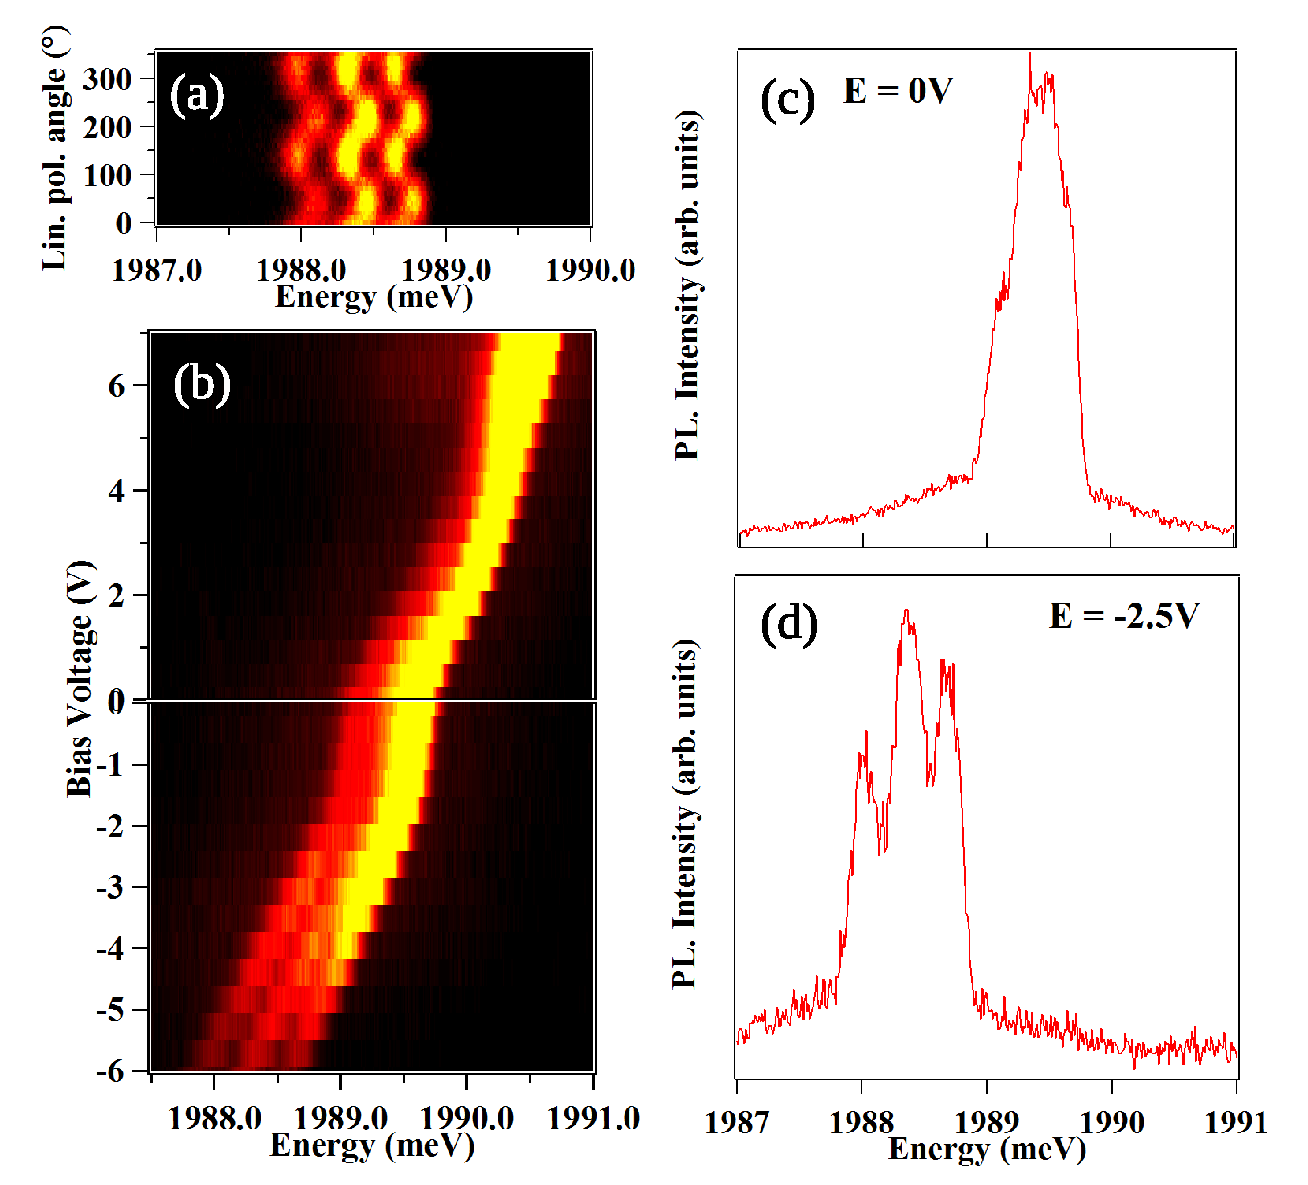
\includegraphics[width=12cm]{04-CrMagOpt/Pictures/SplitUnderEfiledXCr.eps}
	\end{center}
	\caption{All these measures were taken on QD8 X-Cr complex at low temperature. (a) PL intensity dependency in linear polarization. In order to have the best contrast, the map was taken at -2.5V bias voltage. (b) Circular PL intensity evolution in electric field. A splitting began to appear around -2V of applied bias voltage. (c)-(d) Circular PL for an applied bias voltage of, respectively, 0V and -2.5V.}
	\label{CrSixPeaksSplit}
	\end{figure}
		
	Fig.~\ref{CrSixPeaksSplit} shows that, using electric field, we can manipulate the splitting of any given charged state of the QD. For all positive bias voltage between 0V and 7V, X-Cr present a broad emission containing all six peaks in linear emission, as show on Fig.~\ref{CrSixPeaksSplit}(a). The emission then divide into three distinct peaks, starting to appear around -1V. This is evidenced on the the PL emission on Fig.~\ref{CrSixPeaksSplit}(d).
	
	\begin{figure}[h!]
	\begin{center}
		\includegraphics[width=14.9cm]{04-CrMagOpt/Pictures/CrCloseDot.png}
	\end{center}
	\caption{(a) Cr accessible charged states in ZnTe. (b)-(d) Illustration of the effect of a punctual charge on the wavefunction of an electron (red) and a hole (yellow) in a quantum dots.}
	\label{CrOutsideDot}
	\end{figure}
	
	
	We propose that those dots particular PLs are caused by Cr in the ZnTe barrier close to the dot. Cr is incorporated in ZnTe as Cr$^{2+}$, but, as shown on Fig.\ref{CrOutsideDot}(a), the Cr$^+$ and Cr$^{3+}$ states are in the gap and accessible~\cite{CrZnTe}, either by capturing an electron (Cr$^+$) or a hole (Cr$^{3+}$). Considering such a charge close to the QD, it can be viewed as a punctual one, since the dot is far bigger than the atom. The effect on the wave functions, presented in Fig.\ref{CrOutsideDot}(b)-(d), differs depending on the electrical charge of the Cr atom. Cr$^{2+}$ is the neutral state of Cr in ZnTe, sharing its outer shell electrons to bond with the atoms of the crystal. It is therefore the neutral position of the QD-Cr system. Capturing an electron, the Cr atom get a supplementary negative charge, and will thus attract more strongly the hole confined in the QD and repel the electron. The opposite happens when the Cr capture a hole.
	
	The electron is well confined in CdTe/ZnTe quantum dots and is thus not affected strongly by the presence of a punctual charge close to the QD. The hole, on the other hand, is only weakly confined in CdTe/ZnTe QDs. Its wavefunction is then more strongly affected by the charge variations of the Chromium. 
Because of this weak confinement, the hole wavefunction goes slightly out of the dot, and thus may overlap with the Cr atom. Its shape will then be strongly affected by change of charge of the Cr atom atom, being repel when the magnetic atom capture a hole, attracted when it capture an electron. This change in shape of the hole wavefunction affect the exchange interaction with the electron, and thus the emission energy of the exciton. The application of an electric field through the Schottky gate attract the hole toward the surface or the back of the sample, depending on the direction of the applied field. This attraction change the overlap of the hole wavefunction with the Cr atom, reducing it to zero for strong enough electric field. The emission energy is then not affected anymore by the charge variation of the Cr.

	
	
	This hypothesis is currently tested, along with the capacity for the Cr to diffuse outside the quantum dots layer.
	
	\section{Conclusion}
	
	For the first time, a single Cr atom was embedded inside a II-VI quantum dot. We were then able to probe it optically. Such a system presents a characteristic three peak emission, along with the emission of a dark state on the low energy side. The action of the magnetic anisotropy, splitting the Cr spin states according to $D_0 S_z^2$, is strong enough to keep the $S_z = \pm2$ level to be thermally populated, and thus they do not present luminescence. The QDs show a good spin conversation during the exciton lifetime inside the dot, thanks to the effective magnetic field created by the Cr spin. Magneto-optics confirm the chosen energy structure and gives us the possibility to deduce the magnitude of several of the quantum dot parameters. We used the model to simulate the emission of QD with different parameters, and proposed an explanation to the absence of high anisotropy QDs in the one we probed. Some dots seems to correspond to these high anisotropy QDs, but they show no sign of magnetic atom inside them under further investigation. We finished proposing a possible explanation for those dots, supposing the presence of Cr atoms in the ZnTe barrier.
	
	Having successfully inserted a probed single Cr atom in CdTe/ZnTe quantum dots, it is now important to study how this system evolve in time. An important step for further use of the system will be the possibility to prepare the Cr spin in a chosen state, and then control it. This is what we propose to study in the next chapter.


\chapter{Dynamics and optical control of an individual Cr spin in a CdTe QD}
	
	Lorem ipsum dolor sit amet, consectetur adipiscing elit. Curabitur tortor quam, imperdiet quis facilisis sed, fringilla a quam. Cras ante odio, hendrerit ac ante nec, cursus imperdiet urna. Mauris convallis ultricies purus, nec condimentum erat bibendum vel. Aliquam erat volutpat. Pellentesque condimentum, eros a consequat accumsan, turpis sem euismod nisi, sed fringilla quam turpis sit amet erat. Mauris dictum odio sed nisi dapibus, et molestie mauris rutrum. Praesent convallis dolor in nibh blandit bibendum. Quisque sit amet arcu consectetur lorem luctus venenatis nec quis dui. Aliquam erat volutpat. Aenean auctor elit nec tristique dignissim. Nulla massa mi, efficitur semper ex id, pretium eleifend massa. Vivamus sit amet orci scelerisque, gravida est ut, vulputate odio.
	
	\section{Resonant optical pumping and spin dynamics in a Cr doped QD}
	
		\subsection{Resonant optical pumping of the Cr spin}
		
		Lorem ipsum dolor sit amet, consectetur adipiscing elit. Curabitur tortor quam, imperdiet quis facilisis sed, fringilla a quam. Cras ante odio, hendrerit ac ante nec, cursus imperdiet urna. Mauris convallis ultricies purus, nec condimentum erat bibendum vel. Aliquam erat volutpat. Pellentesque condimentum, eros a consequat accumsan, turpis sem euismod nisi, sed fringilla quam turpis sit amet erat. Mauris dictum odio sed nisi dapibus, et molestie mauris rutrum. Praesent convallis dolor in nibh blandit bibendum. Quisque sit amet arcu consectetur lorem luctus venenatis nec quis dui. Aliquam erat volutpat. Aenean auctor elit nec tristique dignissim. Nulla massa mi, efficitur semper ex id, pretium eleifend massa. Vivamus sit amet orci scelerisque, gravida est ut, vulputate odio.
		
	\begin{figure}[h!]
	\begin{center}
		\includegraphics[width=14.7cm]{05-CrDyn/Pictures/PumpPres.png}
	\end{center}
	\caption{Low temperature PL spectra of QD2 exciton in lineraly polarized excitation and detection for B = 0T. No contribution of the charge excitons was found. Inset: Schematic of the energy levels in a Cr-doped QD and configuration of excitation/detection for resonant optical pumping. The ground states $S_z = 0$, $\pm1$ are split by the magnetic anisotropy $D_0 S_z^2$. In the excited state (X-Cr), the exchange interaction with the bright exciton ($|\pm1\rangle$) split the states $S_z = \pm1$.}
	\label{PumpPres}
	\end{figure}
	
	Curabitur eget ipsum egestas dui viverra suscipit. Cras aliquet lacus vitae erat finibus semper. Nulla pharetra eget urna vitae sodales. Nunc faucibus velit lacus, nec ornare eros aliquet quis. Donec a orci nec sem pulvinar ultricies sit amet ut arcu. Nullam id vehicula enim, at tincidunt velit. Duis vestibulum lorem a molestie fringilla. Nullam tincidunt semper placerat. Donec nibh sem, ornare eget cursus ac, luctus sit amet eros. Phasellus eget interdum nisi. Donec mollis risus id lectus fringilla, et commodo risus iaculis. Donec at lacus sed nibh posuere posuere sit amet eget sapien. In dignissim, enim sit amet convallis fermentum, lacus nulla gravida tortor, non facilisis ex nisl sit amet augue. Maecenas eu enim condimentum, consectetur ligula vel, tincidunt nisl. Nam laoreet dictum volutpat. Donec at erat venenatis, ultrices lorem ac, vestibulum neque.
	
	\begin{figure}[h!]
	\begin{center}
		\includegraphics[width=14.7cm]{05-CrDyn/Pictures/ExperimentSchema.png}
	\end{center}
	\caption{Schematic view of the micro-spectroscopy set-up used for the time-resolved optical pumping experiment. The monomode laser is a dye laser tuned on resonance with the studied dot transition, acting as the pump. The other dye laser is tuned on a resonant state, acting as the probe. Both beamsplitters are non-polarizing.}
	\label{PumpExpSetup}
	\end{figure}	
		
	Curabitur eget ipsum egestas dui viverra suscipit. Cras aliquet lacus vitae erat finibus semper. Nulla pharetra eget urna vitae sodales. Nunc faucibus velit lacus, nec ornare eros aliquet quis. Donec a orci nec sem pulvinar ultricies sit amet ut arcu. Nullam id vehicula enim, at tincidunt velit. Duis vestibulum lorem a molestie fringilla. Nullam tincidunt semper placerat. Donec nibh sem, ornare eget cursus ac, luctus sit amet eros. Phasellus eget interdum nisi. Donec mollis risus id lectus fringilla, et commodo risus iaculis. Donec at lacus sed nibh posuere posuere sit amet eget sapien. In dignissim, enim sit amet convallis fermentum, lacus nulla gravida tortor, non facilisis ex nisl sit amet augue. Maecenas eu enim condimentum, consectetur ligula vel, tincidunt nisl. Nam laoreet dictum volutpat. Donec at erat venenatis, ultrices lorem ac, vestibulum neque.
	
	\begin{figure}[h!]
	\begin{center}
		\includegraphics[width=14.7cm]{05-CrDyn/Pictures/PumpResults.eps}
	\end{center}
	\caption{(a) PL transients recorded in circular polarization on line (3) and on line (4) (as defined in the inset) under the resonant (pump on (1)) and quasi-resonant (probe at $E_{exc.}\approx 2068$ meV) optical excitation sequences displayed at the bottom. Inset: PL of X-Cr and configuration of the resonant excitation and detection. (b) and (c): Energy detuning dependence of resonant PL intensity ($I_1$, at the beginning and $I_2$, at the end of the pump pulse) and of the corresponding normalized amplitude of pumping transient $\Delta I/I_2 = (I_1-I_2)/I_2$.}
	\label{PumpingExp}
	\end{figure}		
		
	Curabitur eget ipsum egestas dui viverra suscipit. Cras aliquet lacus vitae erat finibus semper. Nulla pharetra eget urna vitae sodales. Nunc faucibus velit lacus, nec ornare eros aliquet quis. Donec a orci nec sem pulvinar ultricies sit amet ut arcu. Nullam id vehicula enim, at tincidunt velit. Duis vestibulum lorem a molestie fringilla. Nullam tincidunt semper placerat. Donec nibh sem, ornare eget cursus ac, luctus sit amet eros. Phasellus eget interdum nisi. Donec mollis risus id lectus fringilla, et commodo risus iaculis. Donec at lacus sed nibh posuere posuere sit amet eget sapien. In dignissim, enim sit amet convallis fermentum, lacus nulla gravida tortor, non facilisis ex nisl sit amet augue. Maecenas eu enim condimentum, consectetur ligula vel, tincidunt nisl. Nam laoreet dictum volutpat. Donec at erat venenatis, ultrices lorem ac, vestibulum neque.

	\begin{figure}[h!]
	\caption{Optical pumping under a CW probe at $E = 2004$ meV. (a) Pumping on line (1) and detecting on line (4). (b) Pumping on line (4) and detecting on line (1).}
	\label{ContProbe}
	{\begin{center}
		\includegraphics[width=10cm]{05-CrDyn/Pictures/ContProbe.eps}
	\end{center}}
	\end{figure}

	Curabitur eget ipsum egestas dui viverra suscipit. Cras aliquet lacus vitae erat finibus semper. Nulla pharetra eget urna vitae sodales. Nunc faucibus velit lacus, nec ornare eros aliquet quis. Donec a orci nec sem pulvinar ultricies sit amet ut arcu. Nullam id vehicula enim, at tincidunt velit. Duis vestibulum lorem a molestie fringilla. Nullam tincidunt semper placerat. Donec nibh sem, ornare eget cursus ac, luctus sit amet eros. Phasellus eget interdum nisi. Donec mollis risus id lectus fringilla, et commodo risus iaculis. Donec at lacus sed nibh posuere posuere sit amet eget sapien. In dignissim, enim sit amet convallis fermentum, lacus nulla gravida tortor, non facilisis ex nisl sit amet augue. Maecenas eu enim condimentum, consectetur ligula vel, tincidunt nisl. Nam laoreet dictum volutpat. Donec at erat venenatis, ultrices lorem ac, vestibulum neque.
	
	\begin{figure}[h!]
	\begin{center}
		\includegraphics[width=14.8cm]{05-CrDyn/Pictures/PWProbe.eps}
	\end{center}
	\caption{PL transients measured on line (4) while pumping on line (4) at $P_{pump} = 250$ $\mu$W (red) or without pumping (dark). (a) $P_{probe} = 125 $ $\mu$W. (b) $P_{probe} = 250 $ $\mu$W. (c) $P_{probe} = 500 $ $\mu$W.}
	\label{PWProbe}
	\end{figure}	
		
	Curabitur eget ipsum egestas dui viverra suscipit. Cras aliquet lacus vitae erat finibus semper. Nulla pharetra eget urna vitae sodales. Nunc faucibus velit lacus, nec ornare eros aliquet quis. Donec a orci nec sem pulvinar ultricies sit amet ut arcu. Nullam id vehicula enim, at tincidunt velit. Duis vestibulum lorem a molestie fringilla. Nullam tincidunt semper placerat. Donec nibh sem, ornare eget cursus ac, luctus sit amet eros. Phasellus eget interdum nisi. Donec mollis risus id lectus fringilla, et commodo risus iaculis. Donec at lacus sed nibh posuere posuere sit amet eget sapien. In dignissim, enim sit amet convallis fermentum, lacus nulla gravida tortor, non facilisis ex nisl sit amet augue. Maecenas eu enim condimentum, consectetur ligula vel, tincidunt nisl. Nam laoreet dictum volutpat. Donec at erat venenatis, ultrices lorem ac, vestibulum neque.
	
	\begin{figure}
	\fcapside{\caption{Detail of the PL transient measured during the resonant pump pulse for a power $P_{probe} = 250$ $\mu$W. The exponential fit (green) gives a characteristic time of $\tau_{pump} = 60$ ns. The inset presents the evolution of $\tau_{pump}$ as a function of the pumping laser power.}\label{PWPump}}
	{\includegraphics[width=7cm]{05-CrDyn/Pictures/PWPump.eps}}
	\end{figure}	
		
	Curabitur eget ipsum egestas dui viverra suscipit. Cras aliquet lacus vitae erat finibus semper. Nulla pharetra eget urna vitae sodales. Nunc faucibus velit lacus, nec ornare eros aliquet quis. Donec a orci nec sem pulvinar ultricies sit amet ut arcu. Nullam id vehicula enim, at tincidunt velit. Duis vestibulum lorem a molestie fringilla. Nullam tincidunt semper placerat. Donec nibh sem, ornare eget cursus ac, luctus sit amet eros. Phasellus eget interdum nisi. Donec mollis risus id lectus fringilla, et commodo risus iaculis. Donec at lacus sed nibh posuere posuere sit amet eget sapien. In dignissim, enim sit amet convallis fermentum, lacus nulla gravida tortor, non facilisis ex nisl sit amet augue. Maecenas eu enim condimentum, consectetur ligula vel, tincidunt nisl. Nam laoreet dictum volutpat. Donec at erat venenatis, ultrices lorem ac, vestibulum neque.	
	
	\begin{figure}[h!]
	\begin{center}
		\includegraphics[width=14.6cm]{05-CrDyn/Pictures/DistantGap.png}
	\end{center}
	\caption{(a) Evolution of the pumping transient intensity in a pump-probe experiment as a function of the distance between the probe laser and the dot. (b) PL transients recorded for a probe laser at $d = 4$ $\mu$m of the dot. Red: probe on; black: pump off. (c) Evolution of the pumping transient intensity as a function of the probe power, for a probe laser at $d = 4$ $\mu$m of the dot. (d) PL transient recorded for a probe laser at $E_{probe} = 2010$ meV (energy not absorbed neither by the dot nor the barriers). Red: probe on; black: pump off. (e) Evolution of the pumping transient intensity in function of the probe power, for a probe not absorbed in the sample.}
	\label{Heating}
	\end{figure}
	
	Curabitur eget ipsum egestas dui viverra suscipit. Cras aliquet lacus vitae erat finibus semper. Nulla pharetra eget urna vitae sodales. Nunc faucibus velit lacus, nec ornare eros aliquet quis. Donec a orci nec sem pulvinar ultricies sit amet ut arcu. Nullam id vehicula enim, at tincidunt velit. Duis vestibulum lorem a molestie fringilla. Nullam tincidunt semper placerat. Donec nibh sem, ornare eget cursus ac, luctus sit amet eros. Phasellus eget interdum nisi. Donec mollis risus id lectus fringilla, et commodo risus iaculis. Donec at lacus sed nibh posuere posuere sit amet eget sapien. In dignissim, enim sit amet convallis fermentum, lacus nulla gravida tortor, non facilisis ex nisl sit amet augue. Maecenas eu enim condimentum, consectetur ligula vel, tincidunt nisl. Nam laoreet dictum volutpat. Donec at erat venenatis, ultrices lorem ac, vestibulum neque.
	
		
		\subsection{Dynamics of the Cr spin under optical excitation}
		
		
		Lorem ipsum dolor sit amet, consectetur adipiscing elit. Curabitur tortor quam, imperdiet quis facilisis sed, fringilla a quam. Cras ante odio, hendrerit ac ante nec, cursus imperdiet urna. Mauris convallis ultricies purus, nec condimentum erat bibendum vel. Aliquam erat volutpat. Pellentesque condimentum, eros a consequat accumsan, turpis sem euismod nisi, sed fringilla quam turpis sit amet erat. Mauris dictum odio sed nisi dapibus, et molestie mauris rutrum. Praesent convallis dolor in nibh blandit bibendum. Quisque sit amet arcu consectetur lorem luctus venenatis nec quis dui. Aliquam erat volutpat. Aenean auctor elit nec tristique dignissim. Nulla massa mi, efficitur semper ex id, pretium eleifend massa. Vivamus sit amet orci scelerisque, gravida est ut, vulputate odio.
	
	\begin{figure}[h!]
	\fcapside{\caption{Auto-correlation of the PL intensity collected in circular polarization on the X-Cr lines (1), (4) and (5) (as defined in Fig.~\ref{PumpingExp}) and compared with the auto-correlation of the exciton in a non-magnetic QD (black line). The curves are shifted for clarity. For line (1), the auto-correlation is also recorded under a transverse magnetic field (blue line).}\label{AutocorPres}}	
	{\begin{center}
		\includegraphics[width=7cm]{05-CrDyn/Pictures/AutocorPeaks.eps}
	\end{center}}
	\end{figure}	
	
			To observe the time fluctuations of the Cr spin under CW optical excitation, we used the statistics of time arrivals of the photons emitted by a Cr-doped QD given by the second order correlation function g$^{(2)}(\tau)$ of the PL intensity. Fig.~\ref{AutocorExpCr} shows g$^{(2)}(\tau)$ for the lines (1), (3) and (4) recorded in circular polarization. These signals are compared with the auto-correlation obtained for the PL of a non-magnetic QD which is characteristic of a single-photon emitter with a dip (anti-bunching) at short delays. The width of the anti-bunching is given by the lifetime of the emitter and the generation rate of excitons and its depth is limited by the time resolution of the HBT setup. As illustrated in Fig.~\ref{AutocorExpCr}, typical non-magnetic CdTe/ZnTe QDs do not present any significant bunching induced by charge fluctuations \cite{QDAutocor,IndistPhoton}. A similar auto-correlation on a X-Cr PL line still presents a reduced coincidence rate near zero delay, but it is mainly characterized by a large photon bunching with a full width at half maximum (FWHM) in the 20 ns range. This large bunching reflects an intermittency in the emission of a given line of the QD coming from fluctuations of the Cr spin in a 10 ns timescale as it will be confirmed by cross-correlation measurements.

		The amplitude of the bunching reaches 5 for line (1) and is slightly weaker for the lower energy lines. In a simple picture of blinking where the selected QD line can be either in a state ON or OFF, the amplitude of the bunching is given by $\Gamma_{OFF}/\Gamma_{ON}$, ratio of the transition rates from OFF to ON, $\Gamma_{ON}$, and from ON to OFF, $\Gamma_{OFF}$ \cite{SubnanoSpectDiff}. An amplitude of bunching larger than 1 is then expected in a multilevel spin system where, after a spin relaxation, multiple spin-flips are usually required to come back to the initial state ($\Gamma_{ON}<\Gamma_{OFF}$). Let us finally note that the bunching signal is not affected by a weak transverse magnetic field ($B_x=0.42$T in Fig.~\ref{AutocorBandPW}). This confirms the presence of a large strain induced magnetic anisotropy $D_0$ which splits the Cr and X-Cr states and blocks their precession in a magnetic field.
		
	\begin{figure}[h!]
	\fcapside{\caption{Auto-correlation of the PL intensity recorded in circular polarization on the high energy X-Cr line (1) for different excitation powers. The inset shows the corresponding FWHM of the bunching signal versus excitation power.}\label{AutocorPW}}	
	{\begin{center}
		\includegraphics[width=7cm]{05-CrDyn/Pictures/AutocorPw.eps}
	\end{center}}
	\end{figure}
	
	Curabitur eget ipsum egestas dui viverra suscipit. Cras aliquet lacus vitae erat finibus semper. Nulla pharetra eget urna vitae sodales. Nunc faucibus velit lacus, nec ornare eros aliquet quis. Donec a orci nec sem pulvinar ultricies sit amet ut arcu. Nullam id vehicula enim, at tincidunt velit. Duis vestibulum lorem a molestie fringilla. Nullam tincidunt semper placerat. Donec nibh sem, ornare eget cursus ac, luctus sit amet eros. Phasellus eget interdum nisi. Donec mollis risus id lectus fringilla, et commodo risus iaculis. Donec at lacus sed nibh posuere posuere sit amet eget sapien. In dignissim, enim sit amet convallis fermentum, lacus nulla gravida tortor, non facilisis ex nisl sit amet augue. Maecenas eu enim condimentum, consectetur ligula vel, tincidunt nisl. Nam laoreet dictum volutpat. Donec at erat venenatis, ultrices lorem ac, vestibulum neque.
	
	\begin{figure}[h!]
	\begin{center}
		\includegraphics[width=12cm]{05-CrDyn/Pictures/CrosscorFit+B.eps}
	\end{center}
	\caption{(a) Correlation signal of the PL intensity of lines (1) and (4) recorded in the same circular polarization (cross-correlation) for three different excitation powers. The curves are shifted for clarity. The black line is an exponential fit with a characteristic time $\tau=20$ ns. (b) Longitudinal magnetic field dependence of the cross-correlation signal obtained at low excitation power.}
	\label{Crosscor}
	\end{figure}
	
	Curabitur eget ipsum egestas dui viverra suscipit. Cras aliquet lacus vitae erat finibus semper. Nulla pharetra eget urna vitae sodales. Nunc faucibus velit lacus, nec ornare eros aliquet quis. Donec a orci nec sem pulvinar ultricies sit amet ut arcu. Nullam id vehicula enim, at tincidunt velit. Duis vestibulum lorem a molestie fringilla. Nullam tincidunt semper placerat. Donec nibh sem, ornare eget cursus ac, luctus sit amet eros. Phasellus eget interdum nisi. Donec mollis risus id lectus fringilla, et commodo risus iaculis. Donec at lacus sed nibh posuere posuere sit amet eget sapien. In dignissim, enim sit amet convallis fermentum, lacus nulla gravida tortor, non facilisis ex nisl sit amet augue. Maecenas eu enim condimentum, consectetur ligula vel, tincidunt nisl. Nam laoreet dictum volutpat. Donec at erat venenatis, ultrices lorem ac, vestibulum neque.
	
	
		\subsection{Cr spin relaxation in the dark}

		Lorem ipsum dolor sit amet, consectetur adipiscing elit. Curabitur tortor quam, imperdiet quis facilisis sed, fringilla a quam. Cras ante odio, hendrerit ac ante nec, cursus imperdiet urna. Mauris convallis ultricies purus, nec condimentum erat bibendum vel. Aliquam erat volutpat. Pellentesque condimentum, eros a consequat accumsan, turpis sem euismod nisi, sed fringilla quam turpis sit amet erat. Mauris dictum odio sed nisi dapibus, et molestie mauris rutrum. Praesent convallis dolor in nibh blandit bibendum. Quisque sit amet arcu consectetur lorem luctus venenatis nec quis dui. Aliquam erat volutpat. Aenean auctor elit nec tristique dignissim. Nulla massa mi, efficitur semper ex id, pretium eleifend massa. Vivamus sit amet orci scelerisque, gravida est ut, vulputate odio.
		
	\begin{figure}[h!]
	\begin{center}
		\includegraphics[width=12cm]{05-CrDyn/Pictures/RelaxDark.eps}
	\end{center}
	\caption{(a) Time evolution of the PL intensity of line (4) of X-Cr under resonant excitation on line (1) with a circularly polarized excitation pulse. (b) Evolution of the amplitude of the pumping transient $\Delta I/I_2$ as a function of the dark time between the excitation pulses. The black line is an exponential evolution with a characteristic time $\tau_{Cr}=1.7$ $\mu$s}
	\label{RelaxDark}
	\end{figure}		
		
	Curabitur eget ipsum egestas dui viverra suscipit. Cras aliquet lacus vitae erat finibus semper. Nulla pharetra eget urna vitae sodales. Nunc faucibus velit lacus, nec ornare eros aliquet quis. Donec a orci nec sem pulvinar ultricies sit amet ut arcu. Nullam id vehicula enim, at tincidunt velit. Duis vestibulum lorem a molestie fringilla. Nullam tincidunt semper placerat. Donec nibh sem, ornare eget cursus ac, luctus sit amet eros. Phasellus eget interdum nisi. Donec mollis risus id lectus fringilla, et commodo risus iaculis. Donec at lacus sed nibh posuere posuere sit amet eget sapien. In dignissim, enim sit amet convallis fermentum, lacus nulla gravida tortor, non facilisis ex nisl sit amet augue. Maecenas eu enim condimentum, consectetur ligula vel, tincidunt nisl. Nam laoreet dictum volutpat. Donec at erat venenatis, ultrices lorem ac, vestibulum neque.

	\begin{figure}[h!]
	\begin{center}
		\includegraphics[width=14.8cm]{05-CrDyn/Pictures/RelaxHeat.png}
	\end{center}
	\caption{Comparison of the relaxation of the Cr spin after resonant pumping in the line (1) with (red) or without (blue) a probe pulse ($E_{probe} = 2070$ meV). (a) Time resolved PL of line (4) for a resonant pump on line (1) with a probe pulse. (b) $\Delta I/I_2$ in function of the dark time $\tau_{dark}$ measured for the relaxation between the probe and the pump pulses (red) or between two pump pulses (blue). (c) Time resolved PL of line (4) for a resonant pump on line (1) with no probe pulse.}
	\label{RelaxHeat}
	\end{figure}

	The $\Delta I/I$ evolution over dark time is used as a measure of the relaxation of the Cr spin: after a long enough time, both lines should stabilize at the same value.	

	\section{Optical Stark effect on an individual Cr spin}
		
		Lorem ipsum dolor sit amet, consectetur adipiscing elit. Curabitur tortor quam, imperdiet quis facilisis sed, fringilla a quam. Cras ante odio, hendrerit ac ante nec, cursus imperdiet urna. Mauris convallis ultricies purus, nec condimentum erat bibendum vel. Aliquam erat volutpat. Pellentesque condimentum, eros a consequat accumsan, turpis sem euismod nisi, sed fringilla quam turpis sit amet erat. Mauris dictum odio sed nisi dapibus, et molestie mauris rutrum. Praesent convallis dolor in nibh blandit bibendum. Quisque sit amet arcu consectetur lorem luctus venenatis nec quis dui. Aliquam erat volutpat. Aenean auctor elit nec tristique dignissim. Nulla massa mi, efficitur semper ex id, pretium eleifend massa. Vivamus sit amet orci scelerisque, gravida est ut, vulputate odio.	
	
	\begin{figure}[h!]
	\begin{center}
		\includegraphics[width=14.8cm]{05-CrDyn/Pictures/AutlerTownes.png}
	\end{center}
	\caption{Energy level of a Cr-doped quantum dot and formation of the dressed-states. We excite resonantly a given transition of the quantum dot with a continuous monochromatic laser (here the $|S_z = +1\rangle \rightarrow |S_z = +1, X_z = +1\rangle$ transition). Considering a mode of $n$, the levels (Cr, $n$) and (X-Cr, $n-1$) are coherently coupled through absorption and stimulated emission of photon. The Rabi splitting $\Omega_r$ between these two levels can be probed in the cross-polarized PL using a second non-resonant probe (as shown on the right part of the diagram). The splitting observed using a third level is the so-called Autler-Townes splitting.}
	\label{StarkPres}
	\end{figure}	
	
		Lorem ipsum dolor sit amet, consectetur adipiscing elit. Curabitur tortor quam, imperdiet quis facilisis sed, fringilla a quam. Cras ante odio, hendrerit ac ante nec, cursus imperdiet urna. Mauris convallis ultricies purus, nec condimentum erat bibendum vel. Aliquam erat volutpat. Pellentesque condimentum, eros a consequat accumsan, turpis sem euismod nisi, sed fringilla quam turpis sit amet erat. Mauris dictum odio sed nisi dapibus, et molestie mauris rutrum. Praesent convallis dolor in nibh blandit bibendum. Quisque sit amet arcu consectetur lorem luctus venenatis nec quis dui. Aliquam erat volutpat. Aenean auctor elit nec tristique dignissim. Nulla massa mi, efficitur semper ex id, pretium eleifend massa. Vivamus sit amet orci scelerisque, gravida est ut, vulputate odio.
		
	\begin{figure}[h!]
	\begin{center}
		\includegraphics[width=14.9cm]{05-CrDyn/Pictures/StarkSplitDet.png}
	\end{center}
	\caption{(a) PL of X-Cr and configuration of excitation in the resonant optical control experiments. The inset illustrate the laser induced splittings in the ground and excited states for a $\sigma+$ excitation on $|S_z=+1\rangle$. (b) PL intensity maps of lines (5) and (4) for an excitation on (1) as a function of the detuning (top) and of the excitation intensity (bottom). The PL is produced by a second non-resonant laser.}
	\label{StarkSplitandDet}
	\end{figure}		

	Curabitur eget ipsum egestas dui viverra suscipit. Cras aliquet lacus vitae erat finibus semper. Nulla pharetra eget urna vitae sodales. Nunc faucibus velit lacus, nec ornare eros aliquet quis. Donec a orci nec sem pulvinar ultricies sit amet ut arcu. Nullam id vehicula enim, at tincidunt velit. Duis vestibulum lorem a molestie fringilla. Nullam tincidunt semper placerat. Donec nibh sem, ornare eget cursus ac, luctus sit amet eros. Phasellus eget interdum nisi. Donec mollis risus id lectus fringilla, et commodo risus iaculis. Donec at lacus sed nibh posuere posuere sit amet eget sapien. In dignissim, enim sit amet convallis fermentum, lacus nulla gravida tortor, non facilisis ex nisl sit amet augue. Maecenas eu enim condimentum, consectetur ligula vel, tincidunt nisl. Nam laoreet dictum volutpat. Donec at erat venenatis, ultrices lorem ac, vestibulum neque.
	
	\begin{figure}[h!]
	\fcapside{\caption{PL of line (1) and (2) (high energy line) for a laser on resonance with the dark exciton state (5). Inset: PL intensity map of line (1) as a function of the laser detuning around (5).}\label{DarkExcSplit}}	
	{\begin{center}
		\includegraphics[width=7cm]{05-CrDyn/Pictures/StarkDark.eps}
	\end{center}}
	\end{figure}

	Curabitur eget ipsum egestas dui viverra suscipit. Cras aliquet lacus vitae erat finibus semper. Nulla pharetra eget urna vitae sodales. Nunc faucibus velit lacus, nec ornare eros aliquet quis. Donec a orci nec sem pulvinar ultricies sit amet ut arcu. Nullam id vehicula enim, at tincidunt velit. Duis vestibulum lorem a molestie fringilla. Nullam tincidunt semper placerat. Donec nibh sem, ornare eget cursus ac, luctus sit amet eros. Phasellus eget interdum nisi. Donec mollis risus id lectus fringilla, et commodo risus iaculis. Donec at lacus sed nibh posuere posuere sit amet eget sapien. In dignissim, enim sit amet convallis fermentum, lacus nulla gravida tortor, non facilisis ex nisl sit amet augue. Maecenas eu enim condimentum, consectetur ligula vel, tincidunt nisl. Nam laoreet dictum volutpat. Donec at erat venenatis, ultrices lorem ac, vestibulum neque.
	
	\begin{figure}[h!]
	\fcapside{\caption{PL spectra of line (5) for an excitation on line (1) at (a) no detuning and max detuning in each direction, and (b) low and high power. The insets show the splitting of the PL doublet as a function (a) of the laser detuning and (b) of the excitation intensity. The fit is obtained with $\hbar\Omega_r = 100$ $\mu$eV.}\label{FutSplitDet}}	
	{\begin{center}
		\includegraphics[width=7cm]{05-CrDyn/Pictures/StarkFit.png}
	\end{center}}
	\end{figure}
	
	Curabitur eget ipsum egestas dui viverra suscipit. Cras aliquet lacus vitae erat finibus semper. Nulla pharetra eget urna vitae sodales. Nunc faucibus velit lacus, nec ornare eros aliquet quis. Donec a orci nec sem pulvinar ultricies sit amet ut arcu. Nullam id vehicula enim, at tincidunt velit. Duis vestibulum lorem a molestie fringilla. Nullam tincidunt semper placerat. Donec nibh sem, ornare eget cursus ac, luctus sit amet eros. Phasellus eget interdum nisi. Donec mollis risus id lectus fringilla, et commodo risus iaculis. Donec at lacus sed nibh posuere posuere sit amet eget sapien. In dignissim, enim sit amet convallis fermentum, lacus nulla gravida tortor, non facilisis ex nisl sit amet augue. Maecenas eu enim condimentum, consectetur ligula vel, tincidunt nisl. Nam laoreet dictum volutpat. Donec at erat venenatis, ultrices lorem ac, vestibulum neque.
	
	
\printbibliography

\end{document}
